\def\DoNotLoadEpstopdf{}
\documentclass[11pt]{article}
\usepackage[T1]{fontenc}
\usepackage{lmodern}
\usepackage[margin=1.05in]{geometry}
\usepackage{amsmath,amssymb,amsthm,mathtools}
\usepackage{microtype,booktabs,array,enumitem}
\usepackage{url}
\usepackage[dvipsnames]{xcolor}
\usepackage[hypertexnames=false,colorlinks=true,linkcolor=MidnightBlue,citecolor=MidnightBlue,urlcolor=MidnightBlue]{hyperref}
\usepackage{tikz}
\usetikzlibrary{arrows.meta,positioning}
\ifdefined\pdfinfoomitdate\pdfinfoomitdate=1\fi
\ifdefined\pdftrailerid\pdftrailerid{}\fi
\ifdefined\pdfsuppressptexinfo\pdfsuppressptexinfo=15\fi
\numberwithin{equation}{section}
\newtheorem{theorem}{Theorem}[section]
\newtheorem{proposition}[theorem]{Proposition}
\newtheorem{lemma}[theorem]{Lemma}
\newtheorem{corollary}[theorem]{Corollary}
\newtheorem{claim}[theorem]{Claim}
\theoremstyle{definition}
\newtheorem{definition}[theorem]{Definition}
\theoremstyle{remark}
\newtheorem{remark}[theorem]{Remark}
\newtheorem{example}[theorem]{Example}
\DeclareMathOperator{\Tr}{Tr}
\DeclareMathOperator{\diag}{diag}
\DeclareMathOperator{\dist}{dist}
\DeclareMathOperator{\rank}{rank}
\DeclareMathOperator{\spec}{spec}
\DeclareMathOperator{\supp}{supp}
\setlist{itemsep=3pt,topsep=5pt}
\setlength{\emergencystretch}{2em}
\title{Deterministic nonbipartite Ramanujan graphs\\in every fixed degree}
\author{OpenAI}
\date{September 23, 2026}
\hypersetup{
 pdftitle={Deterministic nonbipartite Ramanujan graphs in every fixed degree},
 pdfauthor={OpenAI},
 pdfsubject={A deterministic construction with an exact two-sided spectral bound},
 pdfkeywords={Ramanujan graphs, deterministic algorithms, regular graphs, spectral graph theory}
}
\begin{document}
\maketitle
\begin{abstract}
For every fixed integer $d\ge3$, we give a deterministic algorithm
that constructs a simple nonbipartite $d$-regular Ramanujan graph on every
sufficiently large even number $n$ of vertices. It outputs the full adjacency
list in polynomially many bit operations, with an exponent that may depend on
$d$. Every nonconstant adjacency eigenvalue lies strictly between
$-2\sqrt{d-1}$ and $2\sqrt{d-1}$.
\end{abstract}
\clearpage
\begingroup
\small
\tableofcontents
\endgroup
\clearpage
\section{Introduction}\label{sec:introduction}

Nonconstant adjacency eigenvalues that are small in absolute value make the edge distribution of a
regular graph close to the uniform-density prediction, and thus connect
spectral estimates to expansion \cite{Alon1986}.
The Ramanujan threshold is the sharp asymptotic spectral target in fixed
degree. For a simple $d$-regular graph $G$, its adjacency
matrix $A_G$ has the constant eigenvector $\mathbf1$ with eigenvalue $d$.
The restriction $A_G|_{\mathbf1^\perp}$ measures the remaining spectrum.
Throughout this paper the desired bound is
\[
 \bigl\|A_G|_{\mathbf1^\perp}\bigr\|\le 2\sqrt{d-1}.
\]
Here $2\sqrt{d-1}$ is the spectral radius of the infinite $d$-regular
tree; the Alon--Boppana bound makes it asymptotically optimal
\cite{Alon1986,Nilli1991}. Since $d>2\sqrt{d-1}$ for $d\ge3$, this bound
also forces $G$ to be connected and nonbipartite.

The problem addressed here is to construct such graphs deterministically
at prescribed sizes, without a positive error in the spectral bound.
Our meaning of explicitness is the production of the entire adjacency
list. The degree is fixed throughout the complexity analysis.

\begin{theorem}\label{thm:main}
For every integer $d\ge3$ there are constants $n_0(d)$ and $k_d$ and a
deterministic algorithm with the following property. On input an even
integer $n\ge n_0(d)$, the algorithm outputs the adjacency list of a simple
$d$-regular graph $G$ on $n$ vertices in $O_d(n^{k_d})$ bit operations, and
\[
 -2\sqrt{d-1}<\lambda<2\sqrt{d-1}
 \quad\text{for every eigenvalue $\lambda$ of }A_G|_{\mathbf1^\perp}.
\]
In particular, $G$ is connected and nonbipartite.
\end{theorem}

The exponent and the size threshold may depend on $d$. The statement
concerns all sufficiently large even sizes; it does not assert a
running-time bound polynomial jointly in $n$ and $d$, or a local
adjacency-query algorithm.

\begin{corollary}\label{cor:target-size}
For every fixed $d\ge3$, a deterministic polynomial-time algorithm,
on every sufficiently large integer input $N$, produces a simple
connected nonbipartite $d$-regular Ramanujan graph $G$ with
$N\le |V(G)|\le N+1\le2N$.
\end{corollary}
\begin{proof}
Apply Theorem~\ref{thm:main} to the least even integer $n\ge N$.
\end{proof}

\subsection{Earlier constructions and the exact threshold}

Lubotzky, Phillips and Sarnak and Margulis established arithmetic
constructions attaining the tree threshold in restricted degrees
\cite{LPS1988,Margulis1988}. These constructions obtain their spectral
bounds from arithmetic structure and produce infinite families on
arithmetic sequences of orders. Morgenstern extended the available degrees to $q+1$
for every prime power $q$, including nonbipartite families
\cite{Morgenstern1994}. These exact constructions do not cover every
fixed degree and every prescribed large order simultaneously.

Bilu and Linial introduced a different approach based on graph
two-lifts and signings. A two-lift replaces each vertex by two vertices
and each edge by one of the two matchings between the corresponding
pairs. Its new eigenvalues are those of a signed adjacency matrix,
obtained by assigning a sign $+1$ or $-1$ to each edge.
Their deterministic construction gives an
$O(\sqrt{d\log^3 d})$ bound along iterated lifts
\cite{BL2006}. Marcus, Spielman and Srivastava then used interlacing
polynomials to attain the exact bound for the largest signed eigenvalue.
The bipartite Ramanujan convention excludes both $d$ and $-d$ from the
spectral bound. For bipartite graphs, spectral symmetry also controls the negative edge,
yielding simple bipartite Ramanujan families in every degree
\cite[Theorems~5.3 and~5.5]{MSS2015}.
Hall, Puder and Sawin extended the covering theorem to arbitrary lift
degrees; in particular, simple bipartite $d$-regular Ramanujan graphs
exist on $2dr$ vertices for every positive integer $r$
\cite[Theorem~1.2 and Corollary~2.2]{HPS2018}.

The matching construction of Marcus, Spielman and Srivastava gives
bipartite Ramanujan multigraphs at every even order, with strict bounds
on the eigenvalues other than $\pm d$
\cite[Theorem~1.1]{MSS2018}. Cohen made this construction deterministic
in polynomial time \cite{Cohen2016}. More recently, Cohen and Maor
obtained a quantitative improvement below the tree threshold in this
bipartite multigraph model \cite[Theorem~1.2]{CM2026}.
The restriction to $\mathbf1^\perp$ in Theorem~\ref{thm:main} includes
the negative eigenvalue that bipartiteness would produce.

Recent polynomial expected-time signing algorithms of Jadbabaie,
Saberi and Sra attain the sharp one-sided threshold, and hence the
absolute threshold for bipartite inputs, using a Las Vegas algorithm;
their general two-sided bound has an additional factor $\sqrt2$
\cite[Theorem~6.1]{JSS2026}.
The Bilu--Linial conjecture asks whether every $d$-regular graph has a
two-lift whose new eigenvalues all lie in
$[-2\sqrt{d-1},2\sqrt{d-1}]$ \cite[Conjecture~3.1]{BL2006}.
Our prescribed-order construction uses partial pairings and edge
switches, and does not resolve that signing problem.

For every fixed degree and every fixed $\varepsilon>0$, Mohanty,
O'Donnell and Paredes gave deterministic simple constructions with
bound $2\sqrt{d-1}+\varepsilon$, and order within a factor $1+o(1)$
of a requested size \cite{MOP2020}. Alon obtained this
bound at every sufficiently large size $n$ satisfying $dn$ even
\cite[Theorem~1.3]{Alon2021}. His adjustment of the order deletes
suitably separated vertices from a slightly larger graph and matches
their neighbors; local eigenvector mass estimates control the resulting
spectral error \cite[Section~3]{Alon2021}.
These constructions leave a positive spectral error.
Removing that error requires controlling the eigenvalues on the
much finer scale of their distances from both tree edges.

For every fixed degree and positive error, a uniformly random simple
regular graph is near-Ramanujan with probability tending to one.
This is Friedman's theorem \cite{Friedman2008}; Bordenave gave a new
proof using nonbacktracking operators and extended the method to random
lifts \cite{Bordenave2020}.
Exact existence follows from the joint edge
universality for uniformly random simple regular graphs in every
fixed degree established by Huang, McKenzie and Yau
\cite[Remarks~3.10 and~3.12]{HMY2024}. The probability of the exact two-sided
Ramanujan event tends to approximately $0.69$
\cite[Corollary~1.3]{HMY2024}. Continuity of the
limiting joint edge law gives the same limit for the strict interior
event, so strict existence holds at every sufficiently large
size with $dn$ even. Theorem~\ref{thm:main} supplies a deterministic
polynomial-time construction at the exact threshold and prescribed
even order.

\subsection{How the construction reaches both spectral edges}

Write $q=d-1$, $s=2\sqrt q$ and $e=n^{-2/3+a}$, where $a=10^{-4}$.
The first objective is a simple $d$-regular graph with nonconstant
spectrum in $(-s-e/20,s+e/20)$ and enough local information to repair
the remaining error. An edge switch deletes $\{u,v\}$ and $\{x,y\}$
and inserts $\{u,y\}$ and $\{x,v\}$. It is valid when the four
endpoints are distinct and the inserted edges were absent.
A collection of vertex-disjoint valid switches preserves simplicity,
regularity and the vertex set. A norm bound alone does not determine how
a switch affects an eigenvector concentrated near one of its endpoints.
The construction therefore retains two kinds of local information.

To describe them, let $v_2,\ldots,v_n$ be an orthonormal eigenbasis on
$\mathbf1^\perp$ for this intermediate graph, with eigenvalues
$\lambda_i$, and put $x_i^\sigma=s-\sigma\lambda_i$ for
$\sigma\in\{+1,-1\}$. These signed distances may be slightly negative.
First, the spectral mass near either edge satisfies
\[
 \sum_{i:x_i^\sigma\le w}|v_i(p)|^2\le Cw^{3/2}
 \qquad\text{for every vertex $p$, both signs, and $2e\le w\le2d$}.
\]
Thus the modes requiring repair have little mass at any one vertex.
Summing over vertices also shows that only $O(ne^{3/2})=O(n^{3a/2})$
modes lie within $O(e)$ of either edge. Thus only a small spectral
subspace needs the additional positive bias.
Second, choose one spectrum-avoiding bulk cutoff $w_B^\sigma$ for each sign,
at a prescribed scale larger than $e$, and retain the reciprocal only beyond that cutoff:
\[
 R_B^\sigma=\sum_{i:x_i^\sigma\ge w_B^\sigma}
                  \frac{v_iv_i^T}{x_i^\sigma}.
\]
For all but a small fraction of edges $(p,p')$, the $2$-by-$2$ submatrix
on their endpoints is close, entry by entry, to the tree block
\[
 \frac1{d-2}
 \begin{pmatrix}\sqrt{d-1}&\sigma\\ \sigma&\sqrt{d-1}\end{pmatrix}.
\]
The exceptional edge set may depend on the chosen pair of cutoffs.
This is a local block comparison; the full inverse at the tree edge
need not exist. Theorem~\ref{thm:exact-repair} states the precise scales
and all three repair hypotheses.

The bulk block comparison lets us eliminate the spectral modes beyond
the cutoff and express positivity as a quadratic-form condition on the
remaining near-edge modes. This elimination is a Schur complement.
The original near-edge form can be indefinite. At both edges, a small bias
in the edge-pair distribution gives a positive mean shift to the modes
closest to the threshold; the other near-edge modes retain a fixed
fraction of their positive slack after the mean correction. The local
mass bound controls fluctuations around this mean.
The proof shows that a collection of valid simultaneous switches
satisfying both strict inequalities exists, before giving a finite
deterministic search for it.

\subsection{The four construction stages}

Give each vertex $d$ distinguishable half-edges, called stubs. Pairing
two stubs creates an edge. During the construction we maintain a
positive precision matrix on $\mathbf1^\perp$ for each sign and several
spectral parameters;
at completion these matrices become $zI-\sigma A_G$, with $z>s$ and
$\sigma=\pm1$. Their normalized inverses are compared entry by entry
with truncated weighted sums of nonbacktracking paths, which do not
immediately reverse an edge. Lemma~\ref{lem:discounted-accounts}
selects each pair by minimizing a weighted sum of nonnegative statistics.
Each statistic is discounted by its own computed one-step growth factor,
so the same choice preserves all the required estimates.

\begin{enumerate}
\item \textbf{Pair most stubs.}
Starting from the empty pairing,
Proposition~\ref{prop:early-phase} in Section~\ref{sec:early-phase}
leaves a sparse set of unresolved stubs while preserving positivity,
trace estimates and entrywise comparison. Its main difficulty is simultaneous control
of polynomially many entries over a long sequence of choices.
Lemma~\ref{lem:early-high-moments} bounds the growth of a high moment
with a coefficient independent of the moment order. Taking a
sufficiently large fixed moment therefore gives the required maximum
bound.

\item \textbf{Separate the remaining stubs.}
Given these estimates, Section~\ref{sec:cleanup} pairs the stubs that are close to one another
or to a short return. The surviving stubs occupy distinct vertices,
and no short nonempty nonbacktracking path joins any two of these vertices or
returns to one. The analytic estimates persist during this prescribed
cleanup, by Proposition~\ref{prop:cleanup} and the structural
separation statement in Lemma~\ref{lemma:structure}.

\item \textbf{Complete the graph.}
The separated boundary makes the compression of a smoothly truncated path
reference to unresolved-stub contrasts close to the identity. These contrasts
are vectors of unresolved-stub coordinates whose entries sum to zero. Each vertex row of the
path reference has at most one substantial boundary
coordinate. Exact low-rank inverse updates, given by Woodbury identities,
continue this reference throughout completion.
Section~\ref{sec:boundary-completion} first reduces the squared row
energies and then uses those smaller energies to improve the entry
bounds. This order permits an arbitrary matching of the last few stubs.
Proposition~\ref{prop:boundary-completion} supplies a simple regular
graph with the required spectral confinement and entry comparison
against one smoothly parameterized reference. The construction retains
the path information at the separation stop needed to analyze that
same reference.

\item \textbf{Remove the spectral excess.}
In Section~\ref{sec:exact-repair}, the parameter dependence of the frozen
reference gives the local mass bound in Lemma~\ref{lem:repair-projector};
the retained path information gives the typical endpoint blocks in
Lemma~\ref{lem:repair-bulk}. Together with confinement, these are the
three inputs to Theorem~\ref{thm:exact-repair}. Its biased switches
make both signed precisions strictly positive at $s$ on
$\mathbf1^\perp$, while preserving simplicity, regularity and the
vertex set.
\end{enumerate}

Figure~\ref{fig:construction} summarizes these successive outputs.
\begin{figure}[hbp]
\centering
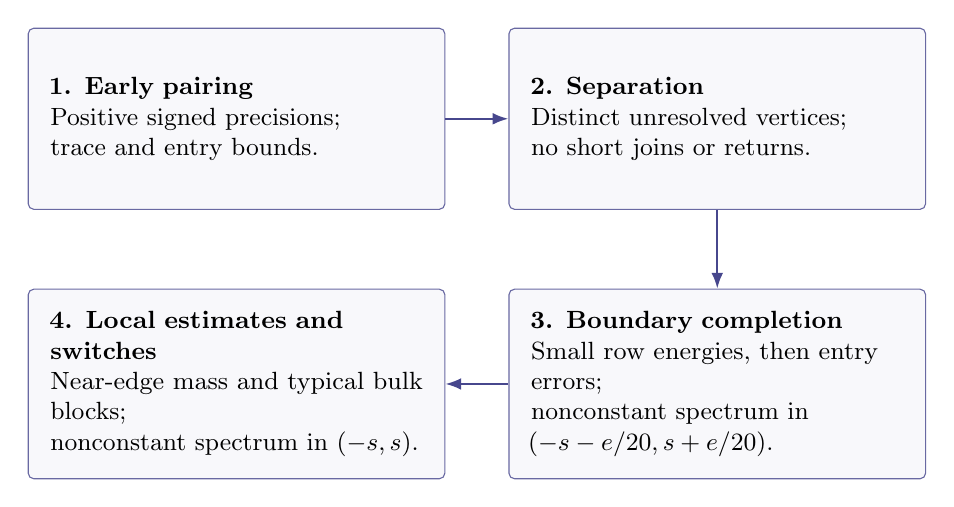
\begin{tikzpicture}[
  box/.style={draw=MidnightBlue!65,fill=MidnightBlue!3,rounded corners=2pt,
    text width=.39\textwidth,minimum height=23mm,inner sep=8pt,align=left,font=\small},
  flow/.style={-{Latex[length=2mm]},thick,draw=MidnightBlue!80}]
\node[box] (early) {\textbf{1. Early pairing}\\
  Positive signed precisions;\\trace and entry bounds.};
\node[box,right=8mm of early] (clean) {\textbf{2. Separation}\\
  Distinct unresolved vertices;\\no short joins or returns.};
\node[box,below=10mm of clean] (complete) {\textbf{3. Boundary completion}\\
  Small row energies, then entry errors;\\nonconstant spectrum in\\
  \mbox{$(-s-e/20,s+e/20)$}.};
\node[box,left=8mm of complete] (repair) {\textbf{4. Local estimates and switches}\\
  Near-edge mass and typical bulk blocks;\\nonconstant spectrum in $(-s,s)$.};
\draw[flow] (early)--(clean);
\draw[flow] (clean)--(complete);
\draw[flow] (complete)--(repair);
\end{tikzpicture}
\caption{The four stages on the same $n$ vertices. The first three
produce the graph and a reference matrix from which the local spectral
estimates for repair are extracted.
Paths in the separation stage are nonempty nonbacktracking paths.
All precisions act on $\mathbf1^\perp$; positivity is tracked for both
spectral signs throughout.}
\label{fig:construction}
\end{figure}


The deterministic selection rule belongs to the method of conditional
expectations and pessimistic estimators \cite{Raghavan1988,WX2008}.
Here each statistic has its own discount, and the transition estimates
control those discounts along the selected history. Weighting a path of
length $j$ by $(\sigma h)^j$ introduces a scalar variable $h$. For a
completed graph, the nonbacktracking path recurrence leads to the quadratic matrix
$I-\sigma hA_G+(d-1)h^2I$, the regular-graph Ihara--Bass pencil
\cite[Sections~6 and~8]{FZ1999}; the partial configuration instead
averages over unresolved stubs, so its identities and quantitative
estimates are proved directly. Likewise, degree-preserving switchings
are classical in regular-graph generation \cite{MW1990}; the local
spectral inputs and the bias that improves both edges are established
in the repair proof.

Local comparison with tree Green functions and stability under edge
resampling were developed by Bauerschmidt, Huang and Yau for random
regular graphs of sufficiently large fixed degree in the bulk
\cite[Sections~2, 7 and~11]{BHY2019}. Huang and Yau extended this
local-resampling approach to every fixed degree $d\ge3$ and obtained
control up to the spectral edges \cite[Sections~1.4, 3 and~5]{HY2024}.
These are methodological precedents for the local comparisons used
here; the estimates along the deterministic pairing history and the
biased simultaneous repair are proved below.

Section~\ref{sec:setup} fixes notation and parameter order;
Section~\ref{sec:accounts} gives the selection principle; and
Section~\ref{sec:foundations} develops the configuration identities
and structural estimates. Section~\ref{sec:algorithm} assembles the
four stages and proves polynomial bit complexity. Its final check is
exact rational positivity of $B^T(4(d-1)I-A_G^2)B$, where the columns
of $B$ form a rational basis of $\mathbf1^\perp$; the repair theorem
ensures that the polynomial search contains a passing candidate.
The structural
enumeration uses color-coding \cite{AYZ1995} and the perfect-hash
families of Naor, Schulman and Srinivasan
\cite[Theorem~3(iii)]{NSS1995}; the weighted configuration estimates
and spectral repair are proved here.

\section{Conventions and parameters}\label{sec:setup}

Throughout the proof $d\ge3$ is fixed, $q=d-1$, $s=2\sqrt q$, and $n$ is
even.  Constants may depend on $d$ and on the fixed parameters and moment
orders chosen below, but never on $n$.  The assertion that a bound has an
arbitrarily small power loss means that, for each prescribed fixed
$\eta>0$, the bound holds with factor $n^\eta$ once its preceding loss
parameters have been chosen sufficiently small and $n$ is sufficiently
large.  A bound denoted $n^{o(1)}$ has this usual meaning for every fixed
positive exponent.  The two uses will be kept distinct when selecting
parameters.

All vertex-space precision matrices and their inverses act on
$\mathbf1^\perp$.  For coordinate entries and traces we extend such an
operator by zero on the constant vector.  Stub-space operators on a
contrast subspace are extended by zero in the same way.  The distinction
between the identity on a contrast subspace and its zero extension is
understood in all compressed identities.

\subsection{Matrices used during the construction}
The matrix estimates use the inverse of a precision matrix assigned to
the current partial pairing; its normalized form will be denoted by $W$.
The first reference, denoted by $P$, is a finite weighted sum of
nonbacktracking paths, with degrees below the cutoff $L$ fixed below.
Through cleanup the entry error is $E=W-P$. At the separated boundary
we replace this path sum by a smooth truncation $\widehat P_0$ and
continue it by exact inverse updates, obtaining $\widehat P$; the error
is then $E=W-\widehat P$. The precise matrix definitions and update
identities begin in Section~\ref{sec:foundations}. No positivity of
$\widehat P$ is needed.

The symbols below are defined in full where their objects first enter
the proof; the table serves as a reference when moving between stages.
\begin{center}
\begin{tabular}{@{}p{.24\textwidth}p{.70\textwidth}@{}}
\toprule
Notation&Meaning and definition\\
\midrule
$S,l$&Current unresolved stubs and their number; Section~\ref{sec:foundations}.\\
$\Xi,\mathcal D$&Centered incidence and $\mathcal D=\Xi\Xi^T$; Section~\ref{sec:foundations}.\\
$M,W$&Signed precision and its normalized inverse; Section~\ref{sec:foundations}.\\
$P,E$&Truncated path sum and $E=W-P$; Lemma~\ref{lemma:configuration-algebra}.\\
$\widehat P,E$&Continued smooth reference and $E=W-\widehat P$; Section~\ref{sec:boundary-completion}.\\
$\Gamma,D$&Stub compression $\Gamma=\Xi^TW\Xi$ and $D=\Gamma-\Pi_l$; $D$ is distinct from $\mathcal D$.\\
$L_0,L_1,\mathcal T$&Centered traces and $\mathcal T=\operatorname{Tr}(\Xi^TW^2\Xi)$; Section~\ref{subsec:resolvent-consequences}.\\
\bottomrule
\end{tabular}
\end{center}

\subsection{Stopping sizes and spectral parameters}
The unresolved-stub counts decrease as
$dn\to l_1\to l_0\to l_2\to l_3\to0$.
The first two stops delimit early pairing and cleanup; $l_2$ separates
the two boundary phases, and $l_3$ is the final arbitrary matching.
Fix $a=10^{-4}$ and put $e=n^{-2/3+a}$.  The following table records the
principal scales.  The relation $\asymp$ permits fixed positive factors
and integer rounding.
\begin{center}
\begin{tabular}{lll}
\toprule
Quantity&Scale&Use\\
\midrule
$l_0$&$n^{2/3+.15a}$&Separated boundary size\\
$b$&$\lceil n^{1/3+.345a}\rceil$&Cleanup steps\\
$l_1$&$l_0+2b$&End of early pairing\\
$q^{L/2}$&$\sqrt{l_0}\,n^{-.29a}$&Path cutoff\\
$q^{R_0}$&$n^{.04a}$&Boundary separation\\
$q^{g_0}$&$n^{.002a}$&Girth exclusion\\
$\alpha_*$&$n^{-1/3+a/2}$&Closest precision parameter\\
$l_2$&$l_0 n^{-g-r}$&End of boundary phase A\\
$l_3$&$n^\chi$&End of concentrated updates\\
\bottomrule
\end{tabular}
\end{center}
The quantities $l_0,l_1,l_2,l_3$ are even.  A logarithmic radius or cutoff
is rounded to an integer, changing its associated power of $q$ by a fixed
factor.  We keep path degrees $<L$.

For $0<h<1/\sqrt q$ define
\[
 z(h)=h^{-1}+qh,\qquad \alpha(h)=1-qh^2,
 \qquad m_h=\frac{h}{1-h^2}.
\]
Choose the largest primary parameter $h_*$ with
$\alpha(h_*)\asymp n^{-1/3+a/2}$ and
$0<z(h_*)-s<e/20$.  Write $\alpha_* = \alpha(h_*)$.
Successive smaller primary parameters have $1-\sqrt qh$ increasing by a
fixed factor, for instance a factor of two, up to a sufficiently small
fixed constant.  Consequently there are $O(\log n)$ primaries, their
$z-s$ scales cover $[e/20,c]$ up to fixed factors, and successive positive
scales have ratios bounded above and bounded away from one.  Every
parameter remains in a fixed compact subinterval of $(0,1)$.

During the early and cleanup phases, add an auxiliary point immediately
below each primary, at distance
\[
 b'=n^{-.16a}\alpha(h).
\]
At the largest primary also use $h_*-j b_h$, $1\le j\le k_h$, where
\[
 b_h=n^{-.03a}\alpha_*,\qquad
 k_h=\left\lceil\frac{10}{.03a}\right\rceil.
\]
The $j$-spacing is exact.  These auxiliary groups are disjoint for large
$n$.  Both signs $\sigma\in\{1,-1\}$ are used at every tracked parameter.
Only the primary points are retained after $l_0$ unresolved stubs remain.

\subsection{Order of the constant choices}\label{subsec:hierarchy}
The stopping sizes and spectral parameters above specify the stages of
the construction. The remaining constants are introduced with the
estimates they control in Sections~\ref{sec:early-phase}--\ref{sec:boundary-completion}.
The following list records the dependencies among those choices, for
reference when checking that every constant is fixed independently of
$n$. In particular, a coefficient governing growth over a whole phase
must be fixed before the higher moment order used to extract an
individual bound. The list is a dependency guide; the indicated later
arguments define the comparators, row bounds, and exceptional events.
\begin{enumerate}
\item Boundary phase A (Section~\ref{subsec:boundary-phase-a}) uses the
fixed $d,a$ and spectral moment order $k=8$. Its initial row bounds have
constants depending only on $d$; the row comparison constants, including
the finite enlargements at exceptional events, are fixed at this stage.
\item The smooth reference of Section~\ref{subsec:boundary-reference}
has a row-tail exponent $r_P>0$; it is permissible to take $r_P=.001a$.
The exponents $g=r>0$ are chosen sufficiently small relative to $a,r_P$
and the finitely many fixed drift constants in phase A. These constants
depend on $k,d$ and the fixed row bounds, not on the higher scalar moment
orders.
\item In phase A the comparator exponent $\zeta_X$ is chosen as in
\eqref{eq:original-50}, followed by $\theta>0$ sufficiently small
compared with $g$. The row-barrier exponents satisfy
$0<r_v<r_s<r_g<r/2$ with strict gaps. The final matching exponent $\chi$
satisfies $g+r\ll\chi<r_P$ and is larger than these row-barrier exponents.
\item In Section~\ref{sec:cleanup}, the exponent $\rho>0$ is small enough
that $20\rho$ is below the separation and scale margins. For each scalar
concentration account, its normalization exponent is smaller than its
drift and variance margins; its fixed even moment order is then chosen
large enough for extraction over its polynomial-size family.
\item For the early high-moment account of
Lemma~\ref{lem:early-high-moments}, a sufficiently large fixed even $p$
is chosen using the uniform growth coefficient in
\eqref{eq:original-33}. Its diagonal weight and outer-entry threshold
are fixed next, determining the finite near radius $R_c$.
The constants used to choose this threshold depend only on $p,d$, the
finite splitting inequalities, and the uniform row bounds.  Constants
depending on the resulting $R_c$ occur only in terms already accompanied
by a negative power of $n$.
\item Finally, the structural and low-square loss exponents are chosen
small enough for these fixed moment orders and for the finite induction
over near radii. The fixed diagram excess cutoff is large enough for all
the moments that have been used.
\end{enumerate}
There is no dependence of a polynomial horizon-growth coefficient on a
later scalar extraction order.  The estimates below record this fact at
the points where it is essential.  All strict comparisons are unchanged
if scales with rational exponents are replaced by dyadic rational
approximations within fixed factors.  Rational choices of the parameters
$h$ with $O_d(\log n)$ bits, including exact equally spaced auxiliaries,
will be used for the algorithm.

\section{Simultaneous deterministic choice}\label{sec:accounts}

A single pairing must preserve several estimates at once. We select it
by minimizing a weighted sum of nonnegative statistics, called accounts.
Each account receives its own discount, computed from its exact
conditional expectation. This separates the common choice from the
different growth estimates used to analyze its consequences.
The underlying method of conditional expectations and pessimistic
estimators is classical \cite{Raghavan1988}; see also
\cite[Section~3]{WX2008}. The lemma below
includes the account-specific discount update in the finite averaging
argument.

\begin{lemma}[Discounted accounts]\label{lem:discounted-accounts}
At a state $x$, let $\Omega(x)$ be a nonempty finite set of candidate
transitions with a specified probability distribution.  For each index
$i$ in a finite set let $Z_i(x)\ge1$ be a nonnegative account and let $D_i>0$ be its current
discount.  Fix nonnegative weights $a_i$.  Set
\[
 r_i=\max\left\{1,\frac{\mathbb E[Z_i(x')\mid x]}{Z_i(x)}\right\},
 \qquad D_i'=D_i/r_i.
\]
There is a candidate $x'$ such that
\[
 \sum_i a_iD_i'Z_i(x')\le\sum_i a_iD_iZ_i(x).
\]
In particular, selecting a minimizer of the left side has this property.
If along the selected history
$\mathbb E[Z_i(x')\mid x]\le(1+c_{i,t})Z_i(x)$ with
$c_{i,t}\ge0$, then
\[
 D_{i,t}^{-1}\le\prod_{j<t}(1+c_{i,j})
 \le\exp\left(\sum_{j<t}c_{i,j}\right)
\]
when the initial discount is one.
\end{lemma}

\begin{proof}
For each index,
$D_i'\mathbb EZ_i(x')\le D_iZ_i(x)$ by definition of $r_i$.
Sum with weights $a_i$ and use that a minimum is no larger than its
average.  The discount product follows from $r_i\le1+c_{i,t}$.
\end{proof}

For a normalized nonnegative estimator $Y$ that can vanish, apply the
lemma to $1+Y$. This convention keeps the expectation ratio defined
and preserves every upper bound obtained by extracting $Y$.

An account attached to a surviving label has value $1+\phi_i\ge1$ while
the label is alive and zero after its death.  The same proof applies up
to death; after death its contribution remains zero and its discount
need not be changed.  When a family contains $F$ labels, each is assigned
the fixed weight $1/F$ from the beginning of the phase.  Hence, if the
discounted total is at most $K$ and a surviving label has
$D_i^{-1}\le B$, then $1+\phi_i\le FKB$.  For a normalized $p$th-power
account this costs the factor $(FKB)^{1/p}$, which is explicitly allowed
when the fixed even order $p$ is chosen.
Scalar trace accounts and aggregate low-square accounts have unit
weight; averaging over the $O(\log n)$ spectral parameters would make no
difference.  Polynomial-size fixed denominators are used for the
individual entry and row families, whose extraction uses high moments.

\begin{lemma}[Scalar upper-excess account]\label{lem:scalar-excess}
Let an alive scalar quantity have current value $X$ and upper threshold
$T$.  On its ordinary next transitions suppose the threshold is unchanged
and, for a fixed scale $b>0$, its increment $\Delta$ satisfies
\[
 |\Delta|\le b,\qquad \mathbb E\Delta\le\mu,
 \qquad\mathbb E\Delta^2\le\nu,
 \qquad\mu,\nu\ge0.
\]
For each fixed even integer $p\ge2$ there is $C_p$ such that the account
$Z=1+((X-T)_+/b)^p$ obeys
\[
 \mathbb EZ'\le
 \left[1+C_p\left(\frac\mu b+\frac\nu{b^2}\right)\right]Z.
\]
The same upper bound holds if the ordinary estimates are conditional on
an event, provided that on each other surviving transition the threshold
is changed so that the account does not increase.  A death transition
may set the account to zero.  For two-sided control apply the assertion
to $X$ and $-X$ separately.
\end{lemma}

\begin{proof}
For real $x$ and $|y|\le1$, Taylor's formula on the positive half-line,
including the possible crossing of zero, gives
\[
 (x+y)_+^p\le x_+^p+p x_+^{p-1}y
       +C_p(1+x_+^{p-2})y^2.
\]
Substitute $x=(X-T)/b$ and $y=\Delta/b$, take expectations, and use
$x_+^j\le1+x_+^p$ for $0\le j\le p$.  On other surviving transitions the
account is bounded by its old value, and on death it is zero.  Averaging
these alternatives gives the same bound without conditioning.
\end{proof}

The later pairing phases use this estimate at a prescribed scale.

\begin{corollary}[Positive-excess account at a prescribed scale]
\label{lem:positive-excess-account}
Let $B_s>0$ and $\lambda>0$. Suppose an alive scalar quantity has an ordinary increment $\Delta$
with $|\mathbb E\Delta|\le\mu$,
$\mathbb E\Delta^2\le\nu$, and $|\Delta|\le\lambda B_s$.
For each fixed even $p\ge2$, the upper-excess account for either
sign, measured in units $\lambda B_s$, has expectation factor at most
\begin{equation}
 1+C_p\left(\frac{\mu}{\lambda B_s}
             +\frac{\nu}{\lambda^2B_s^2}\right).
 \label{eq:original-34}
\end{equation}
The threshold, exceptional-transition, and death conventions are
those of Lemma~\ref{lem:scalar-excess}.
\end{corollary}
\begin{proof}
Apply Lemma~\ref{lem:scalar-excess} with $b=\lambda B_s$ separately
to the quantity and its negative.
\end{proof}

We shall take $\lambda=n^{-\zeta}$. If the sum of the drift and variance
terms in \eqref{eq:original-34} is bounded and the total family size is
polynomial, choosing $p$ sufficiently large makes the excess $o(B_s)$.
More generally a permitted loss $n^C$ in the discount is absorbed by the
same extraction, with $p$ chosen after the fixed exponent $C$ has been
determined.

\subsection{The induction and its accumulated error bounds}
Each transition estimate is proved assuming the current displayed caps.
These caps first imply that every allowed candidate precision remains
positive and that all candidate statistics are defined.  The minimizing
choice then gives the next caps by the preceding lemmas and their stated
extraction margins.  This is an induction on the number of transitions: first define all
candidates from the current estimates, then select a candidate, and
finally extract its estimates from the common sum. The largest discount
loss of one account is never charged to another account.

A pathwise drift budget is used only when it can be bounded for every
prefix of the selected history having the asserted caps.  In cleanup,
earlier actual paths are bounded by actual paths in the graph at the end
of that prefix.  The structural accounts control that graph by a
separate discount estimate that does not use the pathwise drift budget.
Thus the induction first obtains the new structural bounds and then uses
them to bound the accumulated discounts of the remaining accounts.

At a phase boundary the accounts may be reinitialized.  Normalization by
a slightly larger small power than the preceding extraction loss makes
their initial total bounded or $n^{o(1)}$.  The number of spectral
parameters is logarithmic, and all label families are polynomial.  An
additive budget $O(\log n)$ is harmless after a normalization by any fixed
positive power; it is not charged as an unscaled multiplicative error.

\section{Partial configurations and their deterministic estimates}
\label{sec:foundations}

Two kinds of estimates are needed before pairing can proceed. The
structural accounts control actual paths and separate the unresolved
stubs. The analytic estimates turn trace and entry bounds for the
current inverse into the quadratic and moment bounds needed for one
transition. We first derive the common matrix and path identities, then
develop these two sets of estimates. The analytic implications are
conditional: Sections~\ref{sec:early-phase} and~\ref{sec:cleanup} establish
their hypotheses inductively along the selected pairing history.

Throughout this section, an operator on $\mathbf 1^\perp$ is extended by
zero when vertex entries are taken. All constants are uniform in $n$;
they may depend on the fixed parameters chosen in the parameter section.
The notation $n^{o(1)}$ below represents explicitly computable products of
fixed powers of $\log n$ and $\exp(O((\log\log n)^2))$.

\subsection{The configuration pencil and a single exposure}

We begin by assigning a matrix to each partial pairing. Its dependence
on the unresolved stubs will make the change caused by one exposure
explicit.

Give every vertex $d$ distinguished stubs. For a partial pairing, let $S$
be its $l$ unresolved stubs. For $l>0$, let $C_S$ be the vertex--stub
incidence matrix, and put
\[
 t=C_S\mathbf 1,\qquad
 \Pi_l=I-\frac{\mathbf 1\mathbf 1^T}{l},\qquad
 \Xi=C_S\Pi_l,\qquad \mathcal D=\Xi\Xi^T.
\]
Write $\xi_x$ for the column of $\Xi$ indexed by $x$. If $A$ is the
adjacency matrix of the resolved pairs, define
\[
 A_e=A+\frac{tt^T}{l},\qquad
 M(h)=z(h)I-\sigma A_e-h\mathcal D,\qquad
 m_h=\frac{h}{1-h^2},\qquad W=M(h)^{-1}/m_h.
\]
The operators $M(h)$ and $W$ act on $\mathbf 1^\perp$, and $W$ is used
only when $M(h)$ is positive definite. At the empty pairing, $W$ is the
identity on $\mathbf1^\perp$. At a complete pairing, define
$M(h)=z(h)I-\sigma A_G$ and $W=M(h)^{-1}/m_h$ on this subspace;
positivity for both signs
therefore bounds the nonconstant spectrum in absolute value by $z(h)$.
The partial-configuration pencil lets us maintain this positivity during
the exposure. We have $A_e\mathbf 1=d\mathbf 1$
and, writing $\alpha=1-qh^2$,
\[
 -\partial_hM(h)=\mathcal D+h^{-2}\alpha I.
\]

The next lemma identifies the inverse with a formal path generating
function and computes its update when one pair is resolved. Both
descriptions will be used: the path expansion controls entries, and the
matrix update controls the change in the inverse.
For the relation between nonbacktracking walks and the quadratic
Ihara--Bass matrix polynomial, see
\cite[Section~6, Eq.~(6.2)]{FZ1999}. The recurrence below
also includes unresolved averaging blocks, and we prove it directly.

\begin{lemma}[Path generating function and exposure identities]
\label{lemma:configuration-algebra}
Let $C$ be the incidence matrix of all $dn$ stubs. On resolved stubs let
$P_*$ exchange partners, and on $S$ let it be the averaging projection.
Set $D_e=CP_*^2C^T=dI-\mathcal D$ and
\[
 Q_0=I,\qquad
 Q_j=CP_*[(C^TC-I)P_*]^{j-1}C^T\quad(j\ge1).
\]
Then, as a formal power series on $\mathbf 1^\perp$,
\[
 W=\sum_{j\ge0}(\sigma h)^jQ_j.
\]
For distinct $u,v\in S$, $l>2$, define
\[
 U=[\xi_u,\xi_v],\quad
 G_0=I-J_2/l,\quad B=G_0^{-1}=I+J_2/(l-2),\quad
 H_0=-\sigma h FB,
\]
where $J_2$ is the all-ones matrix and $F$ exchanges the two coordinates.
If this pair is resolved, then
\[
 \mathcal D'=\mathcal D-UBU^T,\qquad
 A_e'=A_e+UFBU^T,\qquad
 M'=M+U(hI-\sigma F)BU^T.
\]
With $G=U^TWU$, $D_p=G-G_0$, and
$H=(H_0^{-1}+D_p)^{-1}$, the inverse update, whenever its inverses
exist, is
\[
 W'=W-WUHU^TW.
\]
Uniformly for the prescribed compact range of $h$, if $\|D_p\|=o(1)$,
then $M'>0$ whenever $M>0$.
\end{lemma}

\begin{proof}
We first prove the generating-function identity, then the exposure
formulas and the assertion about positivity.

The matrix $Q_j$ counts weighted nonbacktracking stub walks. A resolved
traversal is deterministic; an unresolved traversal lands uniformly in
$S$, independently on each use. After landing, the arrival stub is
excluded from the next departure. Thus every row sum is $dq^{j-1}$ for
$j\ge1$. Since $P_*^3=P_*$,
\[
 CP_*^2(C^TC-I)P_*=(D_e-I)CP_*.
\]
Expansion gives $Q_1=A_e$, $Q_2=A_e^2-D_e$, and
$Q_j=A_eQ_{j-1}-(D_e-I)Q_{j-2}$ for $j\ge3$. Consequently
\[
 \sum_{j\ge0}(\sigma h)^jQ_j
 =(1-h^2)[I-\sigma hA_e+h^2(D_e-I)]^{-1}=W.
\]
For the exposure identities, write $a=e_{v(u)}$, $b=e_{v(v)}$ and
replace $t$ by $t-a-b$ and $l$ by $l-2$ in
$\mathcal D=\operatorname{diag}(t)-tt^T/l$ and
$A_e=A+tt^T/l$. Direct expansion gives the displayed formulas.
The Woodbury inverse formula \cite{HS1981} applies because
\[
 [m_h(hI-\sigma F)B]^{-1}+G_0=H_0^{-1}.
\]
It remains to verify preservation of positivity.
Both $m_h(hI-\sigma F)B$ and $H_0^{-1}$ have one positive and one
negative eigenvalue, bounded away from zero uniformly in the prescribed
range. The perturbation $D_p=o(1)$ preserves the latter inertia.

We recall the block congruence behind the Schur-complement argument.
For real symmetric blocks $\mathsf A,\mathsf D$ with $\mathsf A$
invertible, and a compatible real rectangular block $\mathsf B$, define
\[
 \mathsf L=
 \begin{bmatrix}I&-\mathsf A^{-1}\mathsf B\\0&I\end{bmatrix}.
\]
Direct multiplication gives
\[
 \mathsf L^T
 \begin{bmatrix}\mathsf A&\mathsf B\\\mathsf B^T&\mathsf D\end{bmatrix}
 \mathsf L
 =\begin{bmatrix}
 \mathsf A&0\\0&\mathsf D-\mathsf B^T\mathsf A^{-1}\mathsf B
 \end{bmatrix}.
\]
Since $\mathsf L$ is invertible, the inertia of the original block
matrix is the sum of the inertias of $\mathsf A$ and
$\mathsf D-\mathsf B^T\mathsf A^{-1}\mathsf B$; here inertia records
the numbers of positive, negative, and zero eigenvalues. When
$\mathsf D$ is invertible, the same identity with the block order
exchanged gives the other Schur complement.

With
$K=(hI-\sigma F)B$, apply the two Schur complements to
$\left[\begin{smallmatrix}M&U\\U^T&-K^{-1}\end{smallmatrix}\right]$.
One complement is $M'$ and the other is
$-m_h(H_0^{-1}+D_p)$, proving that the inertia of $M'$ equals that of
$M$.
\end{proof}

Let $P=P_{<L}$ be the degree-$<L$ truncation of this generating function,
and write $E=W-P$. The formal exposure subtracts the degree-$<L$
truncation of
\begin{equation}
 P U\left[H_0\sum_{j\ge0}
       (-(U^TPU-G_0)H_0)^j\right]U^TP.
 \label{eq:original-1}
\end{equation}
This statement is coefficientwise: every factor $H_0$ has positive
degree, so every coefficient uses only finitely many terms, and every
coefficient of degree less than $L$ is unchanged on replacing $W$ by
$P$.

We will repeatedly use a cancellation that is exact, including the
finite-population correction. For two scalar arrays $a,c$ on $S$, take
an ordered distinct pair uniformly in $I\subseteq S$, where $|I|=l-k$.
Write $a_p=(a(u),a(v))^T$ and $c_p=(c(u),c(v))^T$ for its two-entry
arrays. Their contraction satisfies
\begin{equation}
 \begin{aligned}
 \frac{\mathbb E[a_p^TH_0c_p]}{-2\sigma h}
 &=\frac{(1+1/(l-2))(\sum_Ia)(\sum_Ic)}{|I|(|I|-1)}\\
 &\quad-\frac{k\sum_Iac}{(l-2)|I|(|I|-1)}.
 \end{aligned}
 \label{eq:original-2}
\end{equation}
Indeed, the swap part has average
$2[(\sum_Ia)(\sum_Ic)-\sum_Iac]/[|I|(|I|-1)]$, while the diagonal part
contributes $2\sum_Iac/|I|$. Substituting the coefficients of $FB$
gives \eqref{eq:original-2}. In particular the expectation vanishes for
centered arrays when $I=S$.

\subsection{Structural accounts and separated unresolved stubs}

The path bounds will require control of small graph cores. We construct
accounts for these cores and for proximity among unresolved stubs. The
proximity and return counts identify the stubs that cleanup must resolve
to obtain separation. We verify that cleanup preserves the core bounds.

In the early phase, expose a uniform ordered distinct pair whose
vertices have actual graph distance greater than $g_0$. The graph on
stubs of rejected pairs has maximum degree
$D_g=O_d(q^{g_0})$. Every resulting actual graph is simple and has girth
at least $g_0$.

\begin{lemma}[Structural accounts]
\label{lemma:structure}
Fix $J=\lfloor .9\log_qn\rfloor$ and a sufficiently large fixed integer
$r_*$. The joint discounted-account rule can maintain, through the
early and cleanup phases, the following bound for every connected
multigraph core $H$ of minimum degree at least two, excess
$r=e_H-v_H+1\in\{1,\ldots,r_*\}$, and $s_H=e_H\le r_*J$:
\begin{equation}
 \#\{\text{stub embeddings of }H\}
       \le n^{1-r+o(1)}q^{s_H}.
 \label{eq:original-3}
\end{equation}
An embedding is injective on vertices and uses distinct proper stubs
for all incidences at a vertex. The accounts and their next-step
averages are computable in polynomial time.

At $l=l_1$, fewer than $b$ unresolved stubs are bad, where a stub is bad
if its vertex has a nonempty actual nonbacktracking return of length at
most $R_0$, or lies within distance $R_0$ of another unresolved stub
(including distance zero). Cleanup can resolve all these bad stubs and
stop at $l_0$ with one unresolved stub per unresolved vertex, and no
nonempty actual nonbacktracking path of length at most $R_0$ joining
two unresolved vertices, including a return to one vertex.
\end{lemma}

\begin{proof}
We first construct the core accounts and bound their change under
rejection in the early phase. These bounds give a global path count and,
in particular, the short-return count needed to identify bad stubs. We
then bound proximity, perform cleanup, and verify that cleanup preserves
the same core and path estimates.

\emph{Initial core accounts.}
Suppressing degree-two vertices in a core leaves a bounded-size
multigraph, apart from the separate case of a cycle. Its subdivisions
with at most $r_*J$ edges give $(1+\log n)^{O(r_*)}$ shapes. Cores with
a vertex of degree exceeding $d$ need not be included.

We use the following form of the perfect-hash-family theorem
\cite[Section~4.4, Theorem~3(iii)]{NSS1995}: an $n$-element set has an explicitly
constructible
$k$-perfect family of maps to $k$ colors, of size
$\exp(k) k^{O(\log k)}\log n$, constructible in
$\exp(k) k^{O(\log k)}n^{O(1)}$ time. This is the specialization
$\ell=k$ of their splitter theorem: splitting a $k$-element set
equally among $k$ colors makes the map injective on that set.
The bounded case $k=1$ uses a single constant map.
For $k=v_H$, sum the unrestricted
completion probabilities over embeddings colorful for each map.
Every embedding is included at least once. If an embedding is already
incompatible with the partial pairing it contributes zero; if it has
$p$ demanded pairs still pending, it contributes
\[
 f_p(l)=\prod_{i=1}^p(l-2i+1)^{-1}.
\]
For one coloring the number of colorful ordered vertex assignments is
at most $k!(n/k)^k$. At the empty pairing the proper stub assignments
contribute $\prod_x(d)_{\deg_H(x)}$, where $(d)_j$ is a falling
factorial. Since $e_H\ge v_H$ and $(d)_j\le dq^{j-1}$,
\[
 \frac{\prod_x(d)_{\deg_H(x)}}{d^{e_H}}
 \le d^{v_H-e_H}q^{2e_H-v_H}\le q^{e_H}.
\]
Stirling's estimate cancels the factor $\exp(k)$ against $k!/k^k$,
leaving only a polynomial factor in $k$. Since $k=O_d(\log n)$,
the remaining factor $k^{O(\log k)}\log n$ is $n^{o(1)}$.
The initial account is therefore at most
$n^{1-r+o(1)}q^{s_H}$.

We use color-coding on a bounded-width tree decomposition, following
Alon, Yuster and Zwick \cite[Section~6, Theorem~6.3]{AYZ1995}; the states below also retain
prescribed stub assignments and pending demanded-pair counts. These
colorful sums do not require enumeration of
$n^k$ assignments. Choose a spanning tree of $H$ and a width-one
tree decomposition of that tree. Add the endpoints of the $r$
non-tree edges to every bag. Every edge of $H$ is then covered,
the bags containing each vertex remain connected, and the width
is at most $2r+1=O(r_*+1)$. In a bag record its vertex and stub
assignments, the subset of colors used in the processed part, and the
number of pending demanded pairs. At a join the color subsets must be
disjoint off the bag. At an edge check its two stub statuses and
increment the pending count when appropriate. After totaling by that
count, multiply by $f_p(l)$. There are
$2^{O(k)}n^{O(r_*+1)}$ states and transitions, including joins; all
counts and probabilities have polynomial bit length.

\emph{Change under rejection.}
Under unrestricted exposure this account is a martingale. It remains
to bound the cost of restricting to accepted pairs. Conditional on an
eventual matching
containing $p$ demanded pairs, the next exposed pair is one of these
pairs with total probability $2p/l$; otherwise it is a uniform pair
on the other $l-2p$ stubs. Deleting $2p$ vertices from a rejected-pair
graph of maximum degree $D_g$ changes its rejected-pair proportion by
$O(pD_g/l^2)$. The contribution of demanded hits to a possible
increase in acceptance probability is also $O(pD_g/l^2)$. Bayes'
formula thus bounds the account's conditional expectation by
$1+O(pD_g/l^2)$ times its present value. Summing to $l_1$ costs
$\exp(O(r_*JD_g/l_1))=1+o(1)$. Normalize by
$n^{1-r}q^{s_H}$ and apply the joint account rule.

\emph{Global path diagrams and short returns.}
At every early-phase state, \eqref{eq:original-3} with $r_*>10$,
increased if necessary, bounds a core of excess $r_*$ and at most
$r_*J$ edges by $n^{1-.1r_*+o(1)}<1$. Thus no such actual core occurs.

A connected union of a fixed number of actual nonbacktracking walks,
with total length at most $r_*J$ and a
fixed number of marked endpoints, has excess less than $r_*$. Otherwise
retain a connected subgraph of excess $r_*$ and prune its leaves,
contradicting the absence of such cores just proved. Suppressing unmarked
degree-two vertices leaves boundedly many vertices, so the number of
diagram shapes is $n^{o(1)}$. A diagram with $e'$ edges and excess $r$
has at most
\[
 n^{1-r+o(1)}q^{e'}
\]
embeddings: apply \eqref{eq:original-3} to the core and extend its
bounded-leaf trees at cost $Cq^{e'-s_H}$; for a tree use $Cnq^{e'}$.
The number of walk descriptions in an embedded diagram is bounded by
a constant depending on the fixed parameters. Indeed, branching is
possible only at boundedly many marked or branch vertices, and two
visits to the same such vertex are separated by at least $g_0$ steps.
The ratio $r_*J/g_0$ is bounded independently of $n$.

In particular, the union traced by a nonempty nonbacktracking return
of length $k$ contains a cycle, so its excess is at least one and it has
at most $k$ edges. The global diagram count therefore gives at most
$n^{o(1)}q^k$ such return walks. Summing over $k\le R_0$ and allowing
at most $d$ unresolved stubs at each vertex gives at most
$n^{o(1)}q^{R_0}$ return-bad stubs. This deduction uses only the
early-phase core bound and girth exclusion already established.

\emph{Proximity at the end of the early phase.}
For proximity at $l_1$, count simple paths of lengths $0$ through
$R_0$ with two distinguished, distinct endpoint stubs required to
survive until $l_1$. For an assignment with $p$ pending required pairs
and $r$ marked surviving stubs, its completion probability is
\[
 \frac{(l_1)_r\,2^p((l-l_1)/2)_p}{(l)_{r+2p}},
\]
with value zero for incompatibility. This follows by assigning stubs
to the future pair slots and the final surviving slots of a uniform
permutation. Multiply the contribution by $w^p$, with
$w=1+CD_g/l_1$. A demanded next hit removes one factor $w$ and hence
pays its entire rejection inflation. Conditional on a successful
non-hit, the pair is uniform on the ordinary stubs; deleting the
$2p+r$ distinguished stubs costs only
$1+O((p+r)D_g/l^2)$. The initial normalized colorful sum is
$n^{o(1)}$: without normalization its expectation is
\[
 n^{o(1)}O\left(q^{R_0}\operatorname{polylog}(n)l_1^2/n\right).
\]
For positive-length paths this follows by choosing proper incidences,
paying $(dn)^{-j}(1+o(1))$ for the $j$ edges and
$O((l_1/n)^2)$ for the two surviving flags; length zero obeys the same
bound. Together with the return-bad count above, this bounds all bad stubs.
Both contributions are $o(b)$, since
\[
 q^{R_0}l_1^2/n=n^{1/3+.34a+o(1)},\qquad
 b=n^{1/3+.345a+o(1)}.
\]

\emph{Cleanup.}
The preceding bounds leave enough steps to resolve every bad stub.
Fix the bad set at $l_1$. Resolve each bad stub as first endpoint,
choosing its partner uniformly among surviving initially clean stubs.
Then use any surviving first stub and choose its partner uniformly
among the eligible surviving initially clean stubs until $l_0$; there
are exactly $b$ steps available. An untouched clean
stub is initially farther than $R_0$ from every other unresolved stub.
A path of length at most $R_0$ starting there cannot reach a new
cleanup edge: before its first such edge it would already reach an
initial unresolved vertex in the initial graph. Its short-path and
short-return properties therefore persist. Every cleanup pair is
admissible, and the asserted final separation follows.

It remains to preserve the core accounts during these cleanup steps.
Multiply $f_p(l)$ by
$(1+Cb/l_0)^p$. If the fixed first stub is demanded, success requires
its unique demanded partner; deletion of at most $O(b)$ possible
partners is paid by the lost weight. Otherwise a successful exposure
has probability ratio at most
$f_p(l-2)/f_p(l)=1+O(p/l)$, irrespective of the omissions. The total
discount cost is $\exp(O(r_*Jb/l_0))=1+o(1)$, as is the change on
reinitializing the weights. This completes the simultaneous account
construction. The core bound and girth exclusion therefore hold
through cleanup, so the global diagram and short-return estimates proved
above remain valid there as well.
\end{proof}

\subsection{Path diagrams, absolute majorants, and polynomial tails}

The coefficient majorants and their first-power row bound below hold
in the general partial-configuration setting. The stronger path estimates
are conditional on the current early or cleanup state having $l\ge l_0$,
the core bound \eqref{eq:original-3}, and actual girth at least $g_0$.
Lemma~\ref{lemma:structure} maintains these properties through both
phases; its final separation conclusion is used in
Section~\ref{sec:boundary-completion}. An admissible pair has endpoint
vertices at actual distance greater than $g_0$.

The global diagram bound proved with the structural accounts counts
actual paths over all choices of endpoints. For entrywise inverse
updates we also need bounds with endpoints fixed, and absolute
majorants that include virtual traversals and centering. These
majorants will then control the tail discarded from the formal exposure.

We begin with fixed endpoints. The union of all walks
of length at most $L$ has bounded excess. After the first walk, every walk adding an edge also
increases excess: an added forest would have a new leaf, whereas the
only possible leaves are the already present endpoints. At most
$r_*+1$ walks would witness excess $r_*$. Since $L/J$ is bounded below
one, taking $r_*$ sufficiently large ensures
$(r_*+1)L\le r_*J$, a contradiction. The preceding branch-count
argument consequently bounds the number of walks at each length
between fixed endpoints by a constant. Likewise, a family of
cycle-containing diagrams rooted at $i$, with no possible leaf other
than $i$ and with each total length at most $J$, has bounded excess:
each edge-adding member increases it, including the first member.

\begin{lemma}[Absolute path bounds]
\label{lemma:path-majorants}
In the partial-configuration setting above, let an output label denote
either a vertex coordinate projected onto $\mathbf1^\perp$, or a current
centered stub $\xi_x$. For a label $i$ write
\[
 p_i(x)=P_{i,\xi_x},\quad e_i(x)=E_{i,\xi_x},\quad
 w_i(x)=W_{i,\xi_x}.
\]
We distinguish polynomial coefficient majorants from their numerical
evaluations. Let $N_k(u,v)$ count actual nonbacktracking stub walks of
length $k$ from $u$ to $v$, with $N_0(u,v)=\mathbf1_{u=v}$, and define
the following polynomials with nonnegative coefficients:
\[
 \begin{aligned}
 \mathsf U_l(z)&=\frac{C}{l}
       \left(1+\sum_{k=1}^{L-1}kq^kz^k\right),\\
 \mathsf A_{i,x}(z)&=\sum_{k=0}^{L-1}N_k(v(i),v(x))z^k
                         +\mathsf U_l(z),\\
 \mathsf J_x(z)&=\sum_{k=1}^{L-1}N_k(v(x),v(x))z^k
                         +\mathsf U_l(z),\qquad
 \mathsf B_{x,y}(z)=\mathsf A_{x,y}(z)+C/l.
 \end{aligned}
\]
Here $v(i)$ is the underlying vertex of the output label. The constant
$C$ is large enough to include the virtual, centering, and degree-zero
Gram corrections. Coefficientwise absolute values of $p_i(x)$ are
bounded by $\mathsf A_{i,x}$; diagonal and cross errors of $U^TPU-G_0$
are bounded by $\mathsf J_x$ and $\mathsf B_{x,y}$, respectively.
The actual-walk counts are symmetric, as are these majorants whenever
the input and output are stub labels. Write
\[
 A_i(x)=\mathsf A_{i,x}(h),\qquad
 j_x=\mathsf J_x(h),\qquad b_{xy}=\mathsf B_{x,y}(h).
\]
In particular $\mathsf U_l(h)\le C(1+L)^2q^{L/2}/l$, and
\begin{equation}
 \sum_{x\in S}A_i(x)\le C(1+L)^2q^{L/2}.
 \label{eq:path-row-sum}
\end{equation}

For the following bounds, assume that the current early or cleanup
state has $l\ge l_0$, satisfies \eqref{eq:original-3}, and has actual
girth at least $g_0$. Uniformly through $l_0$,
\begin{equation}
 \begin{split}
 &\sum_{x\in S}A_i(x)^2\le C,\\
 &\sum_{x\in S}j_x^2\le n^\eta,\qquad
   \sum_{x\in S}j_x\le n^\eta q^{L/2}.
 \end{split}
 \label{eq:original-4}
\end{equation}
For an admissible pair in either phase there is a fixed $c_0'>0$ with
\begin{equation}
 j_u+j_v+b_{uv}\le n^{-c_0'}.
 \label{eq:original-5}
\end{equation}
The same decay holds after multiplying nonconstant diagonal
coefficients by any fixed power of their length, including for global
diagonal entries with their degree-zero norm as baseline.
\end{lemma}

\begin{proof}
\emph{Coefficient majorants and the first row sum.}
An entry involving at least one virtual traversal at length $k$ is at
most $Ckq^k/l$: mark one such traversal, sum prefixes by the row sums,
pay its uniform landing factor $1/l$, and sum suffixes backwards using
reversibility and the same row sums. This overcounts and hence is an
upper bound. Vertex centering contributes $dq^{k-1}/n$; averaging an
endpoint against the unresolved stubs contributes at most $Ckq^k/l$.
The length-zero corrections are $O(1/l+1/n)$. These estimates prove the
coefficient majorants and the stated bound on $\mathsf U_l(h)$.
Reversing a walk proves symmetry. For \eqref{eq:path-row-sum}, each
vertex has at most $d$ unresolved stubs, so the actual length-$k$ row
sum is at most $C_dq^k$. Summing with weights $h^k$ and adding
$l\mathsf U_l(h)$ proves the claim. These arguments use no core or
girth hypothesis.

For the remaining estimates we use the stated structural hypotheses.

\emph{Actual-walk row squares.}
First consider actual walks from a fixed vertex to unresolved stubs.
In the squared weighted sum, identical walks contribute at most $d$:
choose the initial departure uniformly among $d$ stubs and successive
departures uniformly among $q$ alternatives, stopping at the first
unresolved departure. A stopped walk of $k$ actual steps has probability
$d^{-1}q^{-k}$, which dominates $d^{-1}h^{2k}$.

For two distinct walks ending at the same unresolved stub vertex,
remove their common terminal segment. Summing the possible common
continuations with squared weights again costs at most $d$ by the
stopping argument. The remaining pair forms a cycle-containing
diagram rooted at the initial vertex, with no other possible leaf.
If its total length $u$ is at most $J$, the rooted-family argument
above bounds its number by $n^{o(1)}$, and $u\ge g_0$ makes its total
weighted contribution $o(1)$. If $J<u\le2L$, take a sufficiently large
fixed $p$-th moment over roots. In a union of $p$ such diagrams every
edge-adding diagram increases excess, so a union of excess $r$ has at
most $\min(p,r)u$ edges. The global embedding bound gives a moment at
most
\[
 n^{1+o(1)}(1+q^u/n)^p.
\]
Here $r_*$ is chosen large enough to cover all $p$ diagrams. Thus each
root's count is at most $n^{1/p+o(1)}(1+q^u/n)$. After multiplication
by $q^{-u/2}$ this is bounded by
\[
 n^{1/p+o(1)}(q^{-J/2}+q^L/n)=o(1)
\]
for, for example, a sufficiently large fixed $p>4$. Summation over
the polylogarithmically many length choices preserves the decay. This proves
the actual row-square bound, with constant depending only on $d$ once
$n$ is large enough.

Adding the virtual and centering terms costs
$O((1+L)^4q^L/l)=o(1)$ in row-square sum, by $l\ge l_0$ and the
prescribed relation between $L$ and $l_0$. Thus the actual-walk bound
also proves the first estimate in \eqref{eq:original-4}.

\emph{Return bounds.}
The global number of return walks of length $k$ is at most
$n^{o(1)}q^k$, proving the first-power bound on $j$. For its square,
pair two return walks of lengths $k,k'$. Excess at least two costs at
most $n^{-1+o(1)}q^{(k+k')/2}$ after weighting, whose sum is $o(1)$.
At excess one the union consists of a root-to-cycle tail and the
cycle. Each return covers all these edges, so their number is at most
$\min(k,k')$; its weighted embedding bound is $n^{o(1)}$. This proves
the return-square bound, after absorbing subpolynomial factors in the
prescribed $n^\eta$.

\emph{Decay at admissible pairs.}
For an admissible pair, girth and endpoint distance exclude all short
nonconstant terms. Bounded fixed-endpoint multiplicity bounds the
remaining sum by $C\sum_{k\ge g_0}q^{-k/2}$, in addition to the
power-small uniform errors. The degree-zero centered Gram error is
$O(1/l)$, even with other stubs at either vertex. Fixed powers of $k$
do not change the resulting positive decay exponent.
\end{proof}

\paragraph{The formal exposure tail.}
The coefficientwise majorants also control the part discarded when
the formal exposure is truncated. At a current early or cleanup state
with $l\ge l_0$, the core bound \eqref{eq:original-3}, and actual girth
at least $g_0$, let $u,v$ be any distinct unresolved stubs. The absolute
coefficient tail of \eqref{eq:original-1}, of total degree at least $L$,
has every entry on global coordinates or current centered-stub labels
bounded by
\begin{equation}
 B_{\rm tail}:=Cq^{-(1/2-\epsilon)L}
       \le n^{.30a}/\sqrt{l_0},
 \label{eq:original-6}
\end{equation}
where $\epsilon>0$ is fixed and sufficiently small, and $C$ may depend
on $\epsilon$.

To prove this, evaluate the nonnegative coefficient majorants at
$z_h=hq^{1/2-\epsilon}\le q^{-\epsilon}<1$. Put
$r=\lfloor g_0/3\rfloor$. Between two fixed vertices there is at most
one actual nonbacktracking walk of length less than $r$, counting all
lengths together: each such walk is simple, and two distinct ones would
form a cycle shorter than $g_0$. This includes the degree-zero walk
when the vertices coincide. Its contribution is at most one. Bounded
fixed-endpoint multiplicity bounds the longer contribution by
$Cz_h^r/(1-z_h)=o(1)$. The rescaled uniform error also tends to zero:
\[
 \mathsf U_l(z_h)\le C(1+L)^2q^{(1-\epsilon)L}/l=o(1),
 \qquad q^L/l_0=n^{-.58a+o(1)}.
\]
Consequently all outer majorants are at most $1+o(1)$. A nonnegative
coefficient majorant $\mathsf D(z_h)$ for the two-by-two middle
deviation $U^TPU-G_0$ has diagonal entries $o(1)$ and off-diagonal
entries at most $1+o(1)$. The degree-zero Gram corrections are $O(1/l)$;
the possible degree-zero off-diagonal contribution for two stubs at the
same vertex is included in the bound by one. Since
\[
 \|\mathsf D(z_h)\|_\infty\le1+o(1),\qquad
 \bigl\lVert z_h(F+J_2/(l-2))\bigr\rVert_\infty
 =z_h\left(1+\frac2{l-2}\right),
\]
the product of the middle and $H_0$ majorants has norm at most
$q^{-\epsilon}(1+o(1))$. For sufficiently large $n$ this is bounded
by a fixed $\rho_\epsilon<1$. Coefficientwise nonnegative matrix
multiplication therefore bounds the whole formal series at $z_h$ by
$C_\epsilon$. Returning to $h$ pays
$q^{-(1/2-\epsilon)L}$ for every term of degree at least $L$.
Finally $q^{-L/2}\asymp n^{.29a}/\sqrt{l_0}$, so choosing
$\epsilon$ sufficiently small proves \eqref{eq:original-6}.
Every fixed power of the number of factor positions is also summable,
since $\sum_{m\ge0}(m+1)^k\rho_\epsilon^m<\infty$ for fixed $k$.
This is a bound on the formal $P$ exposure; it does not assert positivity
after an arbitrary pair is resolved. The actual transitions use
admissible pairs, for which \eqref{eq:original-5} and the entry caps give
the stronger power-small ratio in their numerical mixed expansions.

\subsection{A coefficient bound from positivity of the pencil}

The path estimates control entries of the truncation. Positivity at
both signs supplies an operator bound for each coefficient and hence
for the whole truncation. We derive that bound from the scalar
polynomials obtained by evaluating the pencil on unit vectors.

\begin{lemma}[Polynomial operator bounds]
\label{lemma:pencil-coefficients}
If the precision is positive for both signs at $h$, then
\begin{equation}
 \|h^jQ_j|_{\mathbf1^\perp}\|\le C(1+j)^2,
 \qquad \|P\|\le C(1+L)^3.
 \label{eq:original-7}
\end{equation}
For a fixed stub endpoint, the signed column of $P$ over global
vertices has polylogarithmic squared norm.
For the following absolute column and entry bounds, also assume that
the current early or cleanup state has $l\ge l_0$, satisfies the core
bound \eqref{eq:original-3}, and has actual girth at least $g_0$.
For every fixed integer $p\ge3$, the absolute $p$-power sum of that
column is bounded by a constant; for
sufficiently large $n$ that constant can depend only on $d$ and $p$.
Stub columns have bounded absolute squared sums, and every outer
entry of $P$ in the formal exposure expansion \eqref{eq:original-1} has absolute
value at most $1+o(1)$.
\end{lemma}

\begin{proof}
\emph{Operator bounds.}
On $\mathbf1^\perp$ put
$F(z)=I-zA_e+z^2(qI-\mathcal D)$. For a complex unit vector $v$,
$v^*F(z)v=1-xz+yz^2$ has real $x,y$ and $y\le q$. A nonreal pair of
roots has modulus $y^{-1/2}\ge q^{-1/2}$. A real root in $(-h,h)$ is
also impossible. Endpoint positivity would require another root on
the same side of zero in that interval, but their product would be
less than $h^2\le1/q$, contradicting $1/y\ge1/q$. Linear polynomials
and polynomials with roots of opposite signs are excluded directly
by the endpoint signs. Thus every root has modulus at least $h$.
Factoring the scalar polynomial shows
\[
 |v^*F(z)v|\ge(j+1)^{-2}
 \quad\text{when }|z|=h\left(1-\frac1{j+1}\right),\quad j\ge1.
\]
Since $\|F(z)v\|\ge|v^*F(z)v|$, its inverse has norm at most
$(j+1)^2$. Apply the Cauchy coefficient formula to
$(1-z^2)F(z)^{-1}$; the extra radius ratio is at most a fixed
constant. This proves \eqref{eq:original-7}. Moreover,
$\|\xi_x\|\le C$, so
\[
 \sum_i|P_{i,\xi_x}|^2=\|P\xi_x\|^2
 \le C\|P\|^2\le C(1+L)^6,
\]
where $i$ ranges over global vertices. This proves the signed
column-square bound from positivity alone.

\emph{Column and entry bounds.}
We now combine the operator estimate with the path bounds.
For actual paths of length $j$ to a fixed endpoint, bounded
multiplicity and the total path count give an $\ell^3$ norm
$O(q^{-j/6})$ after weighting, which is summable. Uniform errors have
total cube sum
$O(n[(1+L)^2q^{L/2}/l]^3)=o(1)$. This proves the cubic bound. For the
refined constant, paths shorter than $g_0/3$ are unique in total at
fixed endpoints; their cube sums are at most
$1+\sum_{j\ge1}dq^{j-1}q^{-3j/2}$. Longer actual paths have power-small
supremum and absolute aggregate squared sum $O((1+L)^2)$, so their
$p$-power sums tend to zero. The uniform correction has vanishing
$p$-power sum by its cube bound and vanishing supremum. Apply the triangle inequality in
$\ell^p$. The same short/long separation proves the $1+o(1)$ entry
bound. The cubic column bound has a constant depending only on $d$.
Combining it with the entry bound gives, for every fixed integer $p\ge3$
and all sufficiently large $n$ (depending on $p$),
\[
 \sum_i |P_{i,\xi_x}|^p
 \le (1+o(1))^{p-3}\sum_i |P_{i,\xi_x}|^3
 \le 2C_d.
\]
Here $i$ ranges over global vertex coordinates. Thus the large-power
column constants needed in the early transition
argument can be fixed before its scalar moment order. The same
short/long separation also shows that choosing a fixed distance radius
from a fixed positive entry threshold does not require fixing the later
structural losses first.
\end{proof}

\subsection{Deterministic consequences of the resolvent bounds}
\label{subsec:resolvent-consequences}

This subsection derives deterministic consequences of the trace and entry
bounds in \eqref{eq:original-8}. The transition arguments in the following
sections establish those bounds by induction. At each transition these
implications are applied only to the current state. We first bound the
norm and spectral tail of a positive weighted inverse. We then use
nearby parameter values to obtain local quadratic and averaged trace
estimates, from which the required moments follow. Set
$F_1=\operatorname{Tr}(\mathcal DW)$ and $F_0=\operatorname{Tr}W$.
We use the trace notation
\[
 \begin{gathered}
 \Gamma=\Xi^TW\Xi,\qquad L_1=F_1-(l-1),\qquad L_0=F_0-(n-1),\\
 K_{\rm all}=\Gamma^2,\qquad Q_{\rm all}=\Xi^TW^2\Xi,\qquad
 \mathcal T=\operatorname{Tr}Q_{\rm all}.
 \end{gathered}
\]
At the primaries, the squared-resolvent trace $\mathcal T$ will be kept
away from zero by applying the account rule to its reciprocal.
At all tracked primary and auxiliary points suppose positivity and
\begin{equation}
 |F_1-(l-1)|\le n^{.09a}/\alpha_*,\qquad
 |F_0-(n-1)|\le n^{.12a}/\alpha_*^2,\qquad
 \max_{i,j}|E_{ij}|\le n^{.37a}/\sqrt{l_0},
 \label{eq:original-8}
\end{equation}
where the entries range over the specified global and centered-stub
labels. At a current early or cleanup state with $l\ge l_0$, the core
bound \eqref{eq:original-3}, and actual girth at least $g_0$,
Lemma~\ref{lemma:pencil-coefficients} bounds the formal $P$ outer entries
by $1+o(1)$. The corresponding numerical $W$ outer entries have the
same bound: $W=P+E$, and the entry cap in \eqref{eq:original-8} is
$n^{.37a}/\sqrt{l_0}=o(1)$. Write $v_*=.125a$ and $c=.03a$.

\begin{lemma}[Consequences of the resolvent bounds]
\label{lemma:local-laws-implications}
At a current early or cleanup state, assume $l\ge l_0$, the core
bound \eqref{eq:original-3}, and actual girth at least $g_0$.
Assume positivity and \eqref{eq:original-8} at every tracked primary
and auxiliary parameter, for both signs.
For $B_h^+=\mathcal D+h^{-2}\alpha I$, the positive operator
$S_h=(B_h^+)^{1/2}W(B_h^+)^{1/2}$ has norm at most
$n^{v_*}/\alpha$. For a sufficiently large fixed $C$, the sum of its
eigenvalues above $Cn^c/\alpha$ is at most $n^{v_*}/\alpha$.
These bounds hold at the primaries and their auxiliaries. At all these
points, every global coordinate or centered stub $f$ satisfies
\begin{equation}
 f^TW(\mathcal D+h^{-2}\alpha I)Wf
   \le(1+h^{-2})\|f_\perp\|^2+n^{-c_1}.
 \label{eq:original-10}
\end{equation}
At the primaries, the averaged trace identity is
\begin{equation}
 \frac{\operatorname{Tr}K_{\rm all}}l+
       h^{-2}\alpha\frac{\mathcal T}{l}
       =1+h^{-2}+O(n^{-c_2}).
 \label{eq:original-11}
\end{equation}
The following moment bounds hold at both primaries and auxiliaries:
\begin{equation}
 \begin{split}
 \operatorname{Tr}K_{\rm all}^2+
       \alpha^2\operatorname{Tr}Q_{\rm all}^2
   &\le C\left(n^{2c}l/\alpha^2+n^{4v_*}/\alpha^4\right),\\
 \operatorname{Tr}(\Gamma K_{\rm all})+
       \alpha\operatorname{Tr}(\Gamma Q_{\rm all})
   &\le C\left(n^cl/\alpha+n^{3v_*}/\alpha^3\right),\\
 \|Q_{\rm all}\|&\le Cn^{2v_*}/\alpha^3.
 \end{split}
 \label{eq:original-12}
\end{equation}
The decay exponents $c_1,c_2>0$ are fixed independently of $n$.
\end{lemma}

\begin{proof}
\emph{Reduction to the closest primary.}
We begin with the norm and spectral tail. Positivity at the closest
primary controls the other primary groups directly; the closest group
will require the auxiliary trace bounds.

For every primary group except the closest one, positivity at the
closest point and integration of $-\partial_hM(h)$ give
\[
 M(h)\succeq c_d\alpha(\mathcal D+\alpha I).
\]
Indeed the interval between these points has length comparable with
$\alpha$, and on a fixed subinterval its value of $1-qt^2$ is
comparable with $\alpha$. The claim follows there with norm $C/\alpha$
and an empty tail. It remains to control the closest point.

\emph{A positive finite-difference filter at the closest primary.}
At that point put $R_h=M(h)^{-1}=m_hW$,
$X=(B_h^+)^{-1/2}M(h)(B_h^+)^{-1/2}$ and $S=X^{-1}$. Positivity,
\eqref{eq:original-8}, and $\operatorname{Tr}W=O(n)$ give a polynomial
upper bound on $S$. The bounds $B_h^+\succeq c_d\alpha_*I$ and
$\|M(h)\|=O(1)$ give an inverse-polynomial lower bound. Set
$k=k_h$ and $b=b_h=n^{-c}\alpha_*$.

For the linear pencil $X+xI$, the alternating trace difference at
$0,b,\ldots,kb$ is the nonnegative quantity
\begin{equation}
 \mathcal B:=\sum_{\lambda\in\operatorname{spec}S}
   \lambda\prod_{j=1}^k\frac{jb\lambda}{1+jb\lambda}.
 \label{eq:original-9}
\end{equation}
For $b\lambda$ small, the product suppresses the contribution of
$\lambda$; for $\lambda\ge C/b$, it is bounded below by a positive
constant depending only on $k,C$. A bound on $\mathcal B$ therefore
bounds the spectral tail that we need. We will obtain that bound from
the trace laws for the actual pencil, by comparing its alternating
trace difference with this linear one.

Write the actual pencil in the form $X+xI+\gamma(x)H_*$, where
\[
 H_*=(B_h^+)^{-1},\quad
 \gamma(x)=z(h-x)-z(h)-h^{-2}\alpha_*x,\quad
 T(x)=\operatorname{Tr}[X+xI+\gamma(x)H_*]^{-1}.
\]
Taylor's formula gives $\gamma(x)=O(x^2)$,
$\gamma'(x)=O(x)$, and bounded higher fixed derivatives on the
interval used. At $x=jb_h$, $0\le j\le k_h$, the trace laws imply
\[
 T(x)=m_{h-x}[(l-1)+h^{-2}\alpha_*(n-1)]
          +O(n^{.12a}/\alpha_*).
\]
Consequently,
\[
 \left|\sum_{j=0}^k(-1)^j\binom kjT(jb)\right|
 \le C_k(n^{.12a}/\alpha_*+nb^k).
\]

\emph{Comparison with the linear pencil.}
We show that the preceding trace difference is
$\mathcal B+o(1)+o(\mathcal B)$. The matrices $X$ and $H_*$ need not
commute, so the comparison retains the order of all matrix factors. For
$X_g(x)=X+xI+\gamma(x)H_*$ and $R(x)=X_g(x)^{-1}$,
the divided-difference product rule applied to $RX_g=I$ gives
\[
 R[x_0,\ldots,x_k]
 =\sum_{0=i_0<\cdots<i_p=k}(-1)^p
 R(x_0)\prod_{t=1}^p
 \left(X_g[x_{i_{t-1}},\ldots,x_{i_t}]R(x_{i_t})\right),
\]
where products retain their displayed order and $x_j=jb$. At nonzero
nodes expand about $A_j=(X+jbI)^{-1}$. Because
$\|\gamma(jb)H_*A_j\|\le Cb/\alpha_*=Cn^{-c}$, every such Neumann
series can be truncated at a fixed order $K$ with residual norm
at most $C_Kb^{-1}(Cb/\alpha_*)^K$. After multiplication by $b^k$,
every remaining factor, rank, and initial inverse norm is bounded by
a fixed power of $n$. Choosing $K$ sufficiently large makes the sum
of all residual traces $o(1)$.

After multiplication by $(-1)^kk!b^k$ and taking the trace, the term
with all first divided differences equal to $I$ and all nodes
unperturbed is exactly $\mathcal B$. It remains to show that all other
terms have total absolute value $o(1)+o(\mathcal B)$.
Use a common decomposition into the $O(\log n)$ dyadic spectral
blocks of $S$ for $S$ and every $A_j$, all of which are functions
of $S$. In a nonzero block tuple let
$\lambda_0$ be its largest scale, and let $r_0$ be the rank of a
block at that scale. A cyclic trace is bounded by $r_0$ times the
product of operator norms, by starting the trace at that block.
This choice is available even when the largest block occurs in an
intermediate inverse: cyclicity moves that block to the beginning of
the trace while retaining the cyclic order of all factors.
Write $s_0=\min(\lambda_0,b^{-1})$. The corresponding main scale is,
within constants depending on $k$, $r_0\lambda_0(bs_0)^k$.
This is an upper comparison scale for a mixed block tuple, rather
than the value of that tuple. The initial inverse block has norm at
most $C\lambda_0$, and every nonzero-node inverse block has norm
at most $C_k s_0$, irrespective of where the largest block occurs.
The contribution to $\mathcal B$ from that largest spectral block
is comparable to this scale, since on its dyadic interval
$\lambda\prod_{j=1}^k jb\lambda/(1+jb\lambda)
\asymp_k\lambda_0(bs_0)^k$.

A perturbed first divided difference costs an extra
$O(b/\alpha_*)$. Each Neumann correction costs at most the same.
Replacing $r\ge2$ first divided differences and their intermediate
inverses by a single span-$r$ divided difference costs, relative to
that main scale,
\[
 O\left(\alpha_*^{-1}s_0^{-(r-1)}\right).
\]
If $\lambda_0\ge n^{c/2}/\alpha_*$, every non-main product therefore
has at least one power-small factor, while the other replacement
factors are bounded. Summing the fixed powers of $\log n$ and
charging to the largest block bounds these terms by $o(\mathcal B)$.

Below this threshold, bound absolutely instead. A span-one block,
its following inverse, and one assigned factor $b$ cost
$O(n^{-c/2})$. A higher span $r$ with its following inverse and
$b^r$ costs
\[
 O(b^r\alpha_*^{-1}n^{c/2}/\alpha_*)=O(n^{-rc/2});
\]
the omitted extra factor $\alpha_*^{r-2}n^{-(r-1)c/2}$ is bounded.
Node corrections are bounded as well. The sum of all such tuples is
at most
$n^{1+o(1)}(n^{c/2}/\alpha_*)n^{-kc/2}=o(1)$, by the choice of $k$.
This proves the comparison with the linear pencil.

\emph{Spectral tail and transfer to auxiliaries.}
It follows that $\mathcal B\le C_kn^{.12a}/\alpha_*$. For
$\lambda\ge C/b$, the product in \eqref{eq:original-9} is bounded
below by a positive constant depending only on $k$ and $C$. Hence
the sum above that threshold, and then the norm, are at most
$n^{v_*}/\alpha_*$ for all sufficiently large $n$. Passing between
$S$ and $S_h$ only changes a fixed factor $m_h$. At lower auxiliary
nodes, $M(h-x)^{-1}\preceq M(h)^{-1}$ and
$B_{h-x}^+=(1+o(1))B_h^+$ in relative positive order. The min--max
principle transfers the ordered eigenvalue bounds, increasing the
constant in the tail cutoff.

\emph{Local quadratic estimate.}
The spectral norm bound is now available at all tracked points. We use
it to compare the inverse at a primary with its nearby auxiliary.
If $f$ is a global
coordinate or a centered stub, the path estimates give
$P_{ff}=\|f_\perp\|^2+O(n^{-c_0'})$ and a power-small derivative of
the nonconstant part. Compare $R_h$ and $R_{h-b'}$, where
$b'=n^{-.16a}\alpha$. Their precision difference is
\[
 b'(B_h^+)^{1/2}(I+O(b'/\alpha))(B_h^+)^{1/2}.
\]
The proven norm bound gives
$b'\|S_h\|\le n^{(.125-.16)a}$, a negative power. The resolvent
identity therefore gives the positive quadratic-form comparison
\[
 R_h-R_{h-b'}
 =b'R_h(B_h^+)^{1/2}(I+O(n^{-c'}))(B_h^+)^{1/2}R_h
\]
for some fixed $c'>0$. On a diagonal, the entry error divided by
$b'$ is at most
$Cn^{.53a}/(\alpha_*\sqrt{l_0})=O(n^{-.045a})$.
Using $m_h'/m_h^2=1+h^{-2}$ yields \eqref{eq:original-10} at the
primary.
For a lower auxiliary point at distance $x$, the normalized
precision increment is $x(I+O(x/\alpha))$. Put
$\widetilde S=(B_h^+)^{1/2}R_h(B_h^+)^{1/2}\succeq0$. The map on
the vectors $(B_h^+)^{1/2}R_hf$ has the form
$[I+x\widetilde S T_x]^{-1}$, where
$T_x=I+O(x/\alpha)$ is positive definite. Indeed,
\[
 [I+x\widetilde S T_x]^{-1}
 =T_x^{-1/2}
   [I+xT_x^{1/2}\widetilde S T_x^{1/2}]^{-1}T_x^{1/2}.
\]
The middle factor has norm at most one, so the full norm is at most
$\sqrt{\|T_x\|\|T_x^{-1}\|}=1+O(x/\alpha)$.
Moreover, $B_{h-x}^+$ and $m_{h-x}$ differ from
$B_h^+$ and $m_h$ by relative $O(x/\alpha)$, respectively. Since
$x/\alpha$ is power-small at every auxiliary, these comparisons
transfer \eqref{eq:original-10} to its own normalization at $h-x$,
after reducing $c_1$.
In particular $\sum_xw_i(x)^2\le C$, global unweighted row squares
are at most $C/\alpha$, and $[(\Xi^TW\Xi)^2]_{xx}\le C$.

\emph{Averaged trace identity.}
Take the $\mathcal D$-weighted trace of the same $b'$ resolvent
difference. Its trace-law error after division by $b'l$ is at most
$Cn^{(.09+.16)a}/(l\alpha_*\alpha)$, a negative power. Positivity
and the relative error in the quadratic-form comparison, together
with \eqref{eq:original-10}, give \eqref{eq:original-11}.
Summing the global and stub versions of \eqref{eq:original-10}
also gives $\mathcal T\le C\min(n,l/\alpha)$.

\emph{Moment bounds.}
We now combine the local quadratic estimate with the spectral bulk
and tail bounds. To express the remaining moments in a common matrix,
introduce
$Y=[\Xi,h^{-1}\sqrt\alpha I]$, with the identity projected onto
$\mathbf1^\perp$, and $\mathcal A=Y^TWY$. Its nonzero eigenvalues
are those of $S_h$. Its stub block is $\Gamma$, and the stub block
of $\mathcal A^2$ is $K_{\rm all}+h^{-2}\alpha Q_{\rm all}$,
of trace $O(l)$ by \eqref{eq:original-10}. Split $\mathcal A$ into
its bulk and tail spectral parts. The bulk norm is $O(n^c/\alpha)$;
the tail trace is $O(n^{v_*}/\alpha)$. Their squared parts have
norm $O(n^{2c}/\alpha^2)$ and trace $O(n^{2v_*}/\alpha^2)$,
respectively. Positive compression preserves these bounds.
For a positive bulk compression $C_b$, use
$\operatorname{Tr}C_b^2\le\|C_b\|\operatorname{Tr}C_b$;
for a tail compression $C_t$, use
$\operatorname{Tr}C_t^2\le(\operatorname{Tr}C_t)^2$.
This proves the first estimate in \eqref{eq:original-12}. For the mixed
estimate, split
also the stub block of $\mathcal A$; its bulk contributes
$O(n^cl/\alpha)$, and all terms involving its tail are bounded by
$O(n^{3v_*}/\alpha^3)$, since $c<v_*$. Positive order gives the
last operator bound. Together these estimates prove
\eqref{eq:original-12}.
\end{proof}

\subsection{The estimates passed between pairing stages}

The next two sections establish the hypotheses used above by induction.
The following table records their bounds at the two stopping points;
these are conclusions of Propositions~\ref{prop:early-phase} and
\ref{prop:cleanup}, not additional assumptions. Positivity and the first
three bounds hold for both signs at every tracked primary and auxiliary
parameter. The last bound is needed only at the primaries, and $c_T>0$
denotes a fixed constant.
\begin{center}
\begin{tabular}{@{}lll@{}}
\toprule
Quantity&After early pairing, $l=l_1$&After cleanup, $l=l_0$\\
\midrule
$|L_1|$&$\le n^{.075a}/\alpha_*$&$\le n^{.09a}/\alpha_*$\\
$|L_0|$&$\le n^{.105a}/\alpha_*^2$&$\le n^{.12a}/\alpha_*^2$\\
$\max_{i,j}|E_{ij}|$&$\le n^{.33a}/\sqrt{l_0}$&$\le n^{.37a}/\sqrt{l_0}$\\
$\mathcal T$&$\ge c_T n^{-\theta/2}(n^{-1}+\alpha/l_1)^{-1}$&
 $\ge c_T n^{-\theta}(n^{-1}+\alpha/l_0)^{-1}$\\
\bottomrule
\end{tabular}
\end{center}
The entry labels are global coordinates and surviving centered stubs.
The early bounds leave a positive power of slack inside the caps
\eqref{eq:original-8}; cleanup retains those caps. The structural accounts
also leave fewer than $b$ bad stubs at $l_1$, in the sense of
Lemma~\ref{lemma:structure}. At $l_0$ the unresolved vertices are distinct
and have no nonempty actual nonbacktracking join or return of length at
most $R_0$. Both stages also retain the stub diagonal-square bound
$\sum_{x\in S}E_{xx}^2\le n^\eta$, with a prescribed sufficiently
small fixed loss exponent, and the coefficient and path-multiplicity
bounds. The complete inputs to boundary completion are listed at the
start of Section~\ref{sec:boundary-completion}; only primary parameters
are retained there.

\section{Pairing down to a sparse boundary}\label{sec:early-phase}

We now construct a partial pairing with $l_1$ unresolved stubs. Throughout
this phase, both signed precisions remain positive and their normalized
inverses remain close, entry by entry, to the truncated path matrix $P$.
The structural estimates of the preceding section then leave fewer than
$b$ bad stubs for the separation step to remove.

All conditional expectations in this section are over a uniform ordered
pair of distinct unresolved stubs whose vertices have distance greater than
\(g_0\). A conditional expectation for a surviving output additionally
excludes its one or two stub labels from the selected pair. Global vertex
outputs do not impose this exclusion. The notation \(E_{ij}\) always uses
the vectors attached to the current labels; thus a stub output is centered
using the current unresolved set.

\begin{proposition}[Early pairing]\label{prop:early-phase}
For the fixed parameters of the construction and all sufficiently large
\(n\), the simultaneous discounted-account rule can be run from the empty
pairing down to \(l_1\) unresolved stubs. It retains the structural estimates
\eqref{eq:original-3}--\eqref{eq:original-7}, positivity of every tracked
precision, and, at every tracked point,
\[
 |L_1|\le n^{.075a}/\alpha_*,\qquad
 |L_0|\le n^{.105a}/\alpha_*^2,\qquad
 \max_{i,j}|E_{ij}|\le n^{.33a}/\sqrt{l_0}.
\]
The low-square estimates \eqref{eq:original-23} hold with any prescribed
sufficiently small fixed loss exponent, for any fixed near radius needed
in the proof. At every primary point,
\begin{equation}
 \mathcal T \ \ge\ n^{-\theta/2}(n^{-1}+\alpha/l)^{-1}
\label{eq:original-13}
\end{equation}
after a fixed constant is allowed in the right-hand side.
\end{proposition}

At every exposure, the structural accounts, the trace accounts, the
squared entry sums, and the high entry moments enter the same discounted
total. The proofs below establish their one-step bounds under the common
current-state caps. The squared sums make mixed terms in the high-moment
expansion summably small. A separate weighting of pair and diagonal
moments controls the remaining terms with a drift coefficient independent
of the moment order. This independence permits extraction of a
simultaneous entry bound after a polynomial loss in the discount.

At the empty state, \(W=P=I|_{{\bf1}^\perp}\),
\(L_1=1-d\), \(L_0=0\), and \(\mathcal T=d(n-1)\).
Write
\[
 B_e=n^{.31a}/\sqrt{l_0},\qquad d_m=n^{.33a}/\sqrt{l_0}.
\]
We maintain \(\max|E_{ij}|\le d_m\) together with the squared-sum bounds
stated below; in particular,
\(T_S:=\sum_{x\in S} E_{xx}^2\le n^\eta\), with centered stub indices.
The deterministic implications \eqref{eq:original-8}--\eqref{eq:original-12}
are used only at the current state. There, every valid pair has small
\(D_p\), so its next precisions are positive and the update
\eqref{eq:original-1} is defined. The weighted choice and extraction then
give the displayed caps at the selected next state. This closes the
induction without assuming any candidate's next-state estimates.

\subsection{Trace estimates}

We first control the two trace errors $L_0,L_1$. We also bound
$\mathcal T$ away from zero; this lower bound will provide a strict
margin in the boundary-completion argument. The signed cancellations
needed for these three estimates are collected in the next lemma.

Put \(D=\Gamma-\Pi_l\), a centered full stub matrix with pair block
\(D_p\), and put \(J_{\rm all}=\Gamma Q_{\rm all}\).
In this subsection, \(K,Q,J\) denote the selected pair blocks
of \(K_{\rm all},Q_{\rm all},J_{\rm all}\), respectively.
At the current state,
\begin{equation}
 K_{xx}\le C,\quad Q_{xx}\le C/\alpha,\quad
 \sum_x D_{xx}^2\le n^\eta,\quad \sum_y D_{xy}^2\le C,
\label{eq:original-14}
\end{equation}
by \eqref{eq:original-4}, the squared-sum bound, and
\eqref{eq:original-10}. On valid pairs, \(D_p\) has power-small entries;
on invalid pairs its entries are still bounded. Fixed constants are
included in the expectation-error bounds below. We retain the exact
ordered-distinct denominators in the identities that supply the drift.

\begin{lemma}[Uniform pair contractions]\label{lem:early-pair-contractions}
Let \(A,C\) be centered \(l\)-by-\(l\) matrices, with \(A\) symmetric,
and let a subscript \(p\) denote their \(\{u,v\}\) blocks. For a full
uniform ordered distinct pair,
\[
\begin{split}
 \mathbb E\operatorname{Tr}(H_0A_p)&=0,\\
 \mathbb E\operatorname{Tr}(BA_p)&=\frac{2\operatorname{Tr}A}{l-1},\\
 \mathbb E\operatorname{Tr}(FA_pFC_p)
 &=\frac{2}{l(l-1)}\left(
       \operatorname{Tr}A\operatorname{Tr}C+
       \operatorname{Tr}(AC)-2\sum_x A_{xx}C_{xx}\right).
\end{split}
\]
The last identity remains valid when \(C\) is not symmetric. For a
nonnegative summand, restriction to valid pairs or to survival costs a
factor \(1+O((D_g+1)/l)\). For a signed summand one must also subtract
the omitted pairs before applying this factor.
\end{lemma}
\begin{proof}
Centering gives \(\sum_{u\ne v}A_{uv}=-\operatorname{Tr}A\).
Insert \(B=I+J_2/(l-2)\) and
\(H_0=-\sigma h(F+J_2/(l-2))\) to obtain the first two
identities. Expansion of the last trace gives
\(A_{vv}C_{uu}+A_{uu}C_{vv}+A_{uv}(C_{uv}+C_{vu})\).
Summing its three terms proves the formula. Each stub has at most
\(D_g\) forbidden partners, and survival excludes at most two stubs;
the assertion about restriction follows by counting the available
ordered pairs.
\end{proof}

\begin{lemma}[Trace transition bounds]\label{lem:early-trace-transitions}
Under the current bootstrap bounds, the conditional means and second
moments of the trace errors satisfy
\eqref{eq:original-16}--\eqref{eq:original-18} at all tracked points.
At primary points, \(\mathcal T\) has the lower relative drift
\eqref{eq:original-20}, the second-moment bound
\eqref{eq:early-T-variance}, and relative step size
\(\lvert\Delta\mathcal T\rvert/\mathcal T=o(1)\).
All error constants are uniform in the current state.
\end{lemma}
\begin{proof}

We first compute the two centered trace increments. We then obtain the
three estimates on \(\mathcal T\) needed to bound its reciprocal:
the lower drift, second moment, and maximum relative increment. The terms
containing the possibly large matrix \(J\) require separate estimates.

\emph{The centered trace errors.}

From \(\mathcal D'=\mathcal D-U B U^T\),
\[
 \Delta F_1=-\operatorname{Tr}B G-\operatorname{Tr}H K+\operatorname{Tr}B G H G .
\]
Expand \(H=H_0-H_0 D_p H_0+\cdots\). In the increment of \(L_1\),
the constant \(-2\) cancels the change in its baseline \(l-1\). This gives
\begin{equation}
 \Delta L_1=
 2\operatorname{Tr}H_0 D_p-(1+h^2)\operatorname{Tr}B D_p-\operatorname{Tr}H_0 K
 +\operatorname{Tr}H_0 D_p H_0 K+O(\|D_p\|^2).
\label{eq:original-15}
\end{equation}
Here \(H_0 G_0 H_0=h^2 B\). Under full uniform distinct sampling, the
linear \(H_0\) contractions vanish and
\(\mathbb E\operatorname{Tr}B D_p=2L_1/(l-1)\).
The swap-swap term has diagonal contribution
\(2 h^2 L_1\operatorname{Tr}K_{\rm all}/[l(l-1)]\), with same-index
corrections \(O(1/l)\). Its remaining cross contribution is bounded by
\(C(\operatorname{Tr}\Gamma^3+l)/l^2\); the \(O(1/l)\) changes in swap
entries also cost \(O(1/l)\).

To restrict these polynomial terms to valid pairs, subtract an absolute
error \(O(D_g/l)\) and divide by \(1-O(D_g/l)\). The remaining inverse
series has expectation \(O(n^\eta/l)\) by \eqref{eq:original-14}.
Consequently,
\begin{equation}
 \mathbb E\Delta L_1=a_l L_1+
 O\!\left((n^\eta+D_g)/l+n^c/(l\alpha)+n^{3v_*}/(l^2\alpha^3)\right),
 \quad
 -C/l\le a_l\le n^{-c_3}/l
\label{eq:original-16}
\end{equation}
for some \(c_3>0\). Before conditioning, the coefficient is
\(\frac{2}{l-1}[h^2(\operatorname{Tr}K_{\rm all}/l-1)-1]\).
Its stated bounds follow from the averaged upper bound in
\eqref{eq:original-10} and \(\|\xi_x\|^2=1+O(1/l)\).
The positive normalization for valid pairs preserves these upper and
lower bounds. Also,
\begin{equation}
 \mathbb E(\Delta L_1)^2\le C\big(n^{2c}/(l\alpha^2)+n^{4v_*}/(l^2\alpha^4)+n^\eta/l\big).
\label{eq:original-17}
\end{equation}
Indeed, the ideal \(K_{uv}\) term uses \eqref{eq:original-12}, while
diagonal same-end ideal terms have coefficient \(O(1/l)\).
All other terms use \eqref{eq:original-14}.

For the global trace, \(\Delta L_0=-\operatorname{Tr}H Q\).
The ideal centered term has zero full mean. The term with a single
\(D_p\) between pure swaps has diagonal main contribution at most
\(C|L_1|/(l\alpha)\). Its cross contribution is bounded using
\(\operatorname{Tr}(\Gamma+\Pi_l)Q_{\rm all}\), together with the
same-index corrections. The remainder is \(O(n^\eta/(l\alpha))\).
Thus, on valid choices,
\begin{equation}
\begin{split}
 |\mathbb E\Delta L_0|&\le C\big((|L_1|+n^\eta+D_g)/(l\alpha)
       +n^c/(l\alpha^2)+n^{3v_*}/(l^2\alpha^4)\big),\\
 \mathbb E(\Delta L_0)^2&\le C\big(n^{2c}/(l\alpha^4)+n^{4v_*}/(l^2\alpha^6)
                               +n^\eta/(l\alpha^2)\big).
\end{split}
\label{eq:original-18}
\end{equation}
The contractions used here can be read directly from
Lemma~\ref{lem:early-pair-contractions}: for \(K_{\rm all}=\Gamma^2\),
\(\operatorname{Tr}(DK_{\rm all})=
\operatorname{Tr}(\Gamma^3)-\operatorname{Tr}(\Gamma^2)\), and for
\(Q_{\rm all}\succeq0\),
\(\lvert\operatorname{Tr}(DQ_{\rm all})\rvert
\le\operatorname{Tr}(\Gamma Q_{\rm all})+\mathcal T\).
The diagonal exclusions are bounded using
\(K_{xx}\le C\), \(Q_{xx}\le C/\alpha\), and
\(\sum_x|D_{xx}|\le n^{\eta/2}\sqrt l\).
Terms with two or more \(D_p\) factors have absolute value at most
\(C\|D_p\|^2\), respectively \(C\|D_p\|^2/\alpha\), because
the remaining inverse series is geometric. Their expectations are
bounded by \eqref{eq:original-14}. The ideal variances are
\(C\operatorname{Tr}(K_{\rm all}^2)/l^2\) and
\(C\operatorname{Tr}(Q_{\rm all}^2)/l^2\), respectively; applying
\eqref{eq:original-12} gives exactly the first two summands of
\eqref{eq:original-17} and \eqref{eq:original-18}.

\emph{Lower drift of \(\mathcal T\).}
To prove \eqref{eq:original-13}, we will control the reciprocal statistic.
We first bound \(\mathbb E\Delta\mathcal T\) from below.
The exact update of $\mathcal T$ is
\begin{equation}
 \Delta\mathcal T=
 -\operatorname{Tr}\big[B(I-GH)Q(I-HG)\big]-2\operatorname{Tr}H J
       +\operatorname{Tr}H Q H K .
\label{eq:original-19}
\end{equation}
Using \(G_0,H_0\) in the outer terms, their full-pair mean divided by \(\mathcal T\) is
\[
 \frac{2}{l-1}\,[h^2(\operatorname{Tr}K_{\rm all}/l-1)-1]
       + O((1+\|\Gamma\|^2)/l^2).
\]
For the first outer term, expand \(I-G_0H_0=I+\sigma h F\).
The centered \(F B\) term averages to zero, and the other contribution is
\(-2(1+h^2)/(l-1)\). For the last term, use the same opposite-diagonal
swap average. Its cross trace satisfies
\(\operatorname{Tr}K_{\rm all} Q_{\rm all}\le\|\Gamma\|^2\mathcal T\);
the diagonal exclusions and \(O(1/l)\) swap errors use \(K_{xx}\le C\).

At primaries, \eqref{eq:original-11} therefore bounds this relative drift
below by \(-C\alpha\mathcal T/l^2 -n^{-c_4}/l\). Pair smallness and
\eqref{eq:original-14} bound the change from the ideal outer terms, on
valid pairs, by \(n^{-c_4}\operatorname{Tr}Q\), decreasing
\(c_4>0\) if necessary. The invalid ideal contributions have average
\(O(D_g\mathcal T/l^2)\).

For the \(J\) term, the ideal contraction \(H_0J\) has zero full
mean. In the term with one deviation, \(H_0D_pH_0J\), diagonal
factorization uses
\(\operatorname{Tr}J_{\rm all}=\operatorname{Tr}\Gamma Q_{\rm all}\),
and the cross trace uses \(D=\Gamma-\Pi_l\). The swap average is
therefore bounded by
\[
 C\bigl(|L_1|\|\Gamma\|+\|\Gamma\|^2+\|\Gamma\|\bigr)
       \mathcal T/l^2,
\]
apart from same-index exclusions, invalid pairs, and the
\(O(1/l)\) changes in the swap coefficients. This main bound is
power-small relative to \(\mathcal T/l\), since
\(\lvert L_1\rvert\le n^{.075a}/\alpha_*\) and
\(n^{2v_*}/(l\alpha_*^2)\ll1\).

To handle the exclusions and coefficient changes, including the
invalid-pair part of the ideal \(J\) contraction, use
\[
 |J_{xy}|\le C\sqrt{(Q_{\rm all}^2)_{yy}},\quad
 \sum_y\sqrt{(Q_{\rm all}^2)_{yy}}\le C n^{v_*}\alpha^{-3/2}\sqrt{l\mathcal T}.
\]
Their mean, divided by \(\mathcal T/l\), is at most
\[
 \frac{C(D_g+1)n^{v_*}}{\alpha^{3/2}\sqrt{l\mathcal T}},
\]
which is power-small under the current lower bound
\eqref{eq:original-13}. Finally, terms with at least two deviations
use \(\mathbb E_{\rm valid}\|D_p\|^2\le Cn^\eta/l\) and
\(\max|J_{xy}|\le Cn^{v_*}/\alpha^2\); their contribution is
also power-small relative to \(\mathcal T/l\). Conditioning on
valid pairs preserves the resulting lower drift bound. We have proved
\begin{equation}
 \mathbb E\Delta\mathcal T/\mathcal T \ \ge\ -C\alpha\mathcal T/l^2-n^{-c_4}/l
\label{eq:original-20}
\end{equation}
with some \(c_4>0\), for sufficiently small \(\theta,\eta\).

\emph{Second moment and maximum increment of \(\mathcal T\).}
In \eqref{eq:original-19}, the outer terms are bounded by
\(C\operatorname{Tr}Q\), giving second moment
\(C\mathcal T/(\alpha l)\). The off-diagonal \(J\) terms use
\(\|\Gamma Q_{\rm all}\|_F^2\le
Cn^{4v_*}\mathcal T/\alpha^5\).
For a diagonal \(J_{uu}\), the coefficient \(H_{uu}\) has
conditional squared average at most \(Cn^\eta/l\) over a uniform
valid partner. Indeed, expansion around \(H_0\) gives
\begin{equation}
 |H_{uu}|\le C(1/l+|D_{vv}|+|D_{uv}|)
\label{eq:original-21}
\end{equation}
on valid pairs: the first pure swap from \(u\) touches \(v\),
all other factors are uniformly small, and a non-pure initial swap
costs \(O(1/l)\). The conditional claim follows from
\eqref{eq:original-14} and \(D_g\ll l\). Also, the norm bound
times the trace gives
\[
 \sum_u J_{uu}^2\le C\operatorname{Tr}Q_{\rm all}^2
       \le Cn^{2v_*}\mathcal T/\alpha^3.
\]
Consequently,
\begin{equation}
 \mathbb E(\Delta\mathcal T)^2\le C\left(\frac{\mathcal T}{\alpha l}+
       \frac{n^{4v_*}\mathcal T}{\alpha^5 l^2}
       +\frac{n^{2v_*+\eta}\mathcal T}{\alpha^3 l^2}\right).
\label{eq:early-T-variance}
\end{equation}
Individually, \(\lvert\Delta\mathcal T\rvert\le
Cn^{v_*}/\alpha^2\ll\mathcal T\) under
\eqref{eq:original-13}.
\end{proof}

\begin{lemma}[Trace control by weighted choice]\label{lem:early-trace-accounts}
The trace-square accounts and the inverse-\(\mathcal T\) account have
bounded discount loss under the bootstrap bounds and imply the trace
conclusions of Proposition~\ref{prop:early-phase} with a positive power
of slack.
\end{lemma}
\begin{proof}
\emph{Trace-square accounts.}
Track \(1+L_i^2/S_i^2\), where
\(S_1=n^{.065a}/\alpha_*\) and
\(S_0=n^{.095a}/\alpha_*^2\).
In \eqref{eq:original-16}, the coefficient contribution to square drift
is at most \(2n^{-c_3}L_1^2/l\). Use
\(2|L|/S\le1+L^2/S^2\) for each additive mean error.
Since \(\sum l^{-1}=O(\log n)\),
\(\sum l^{-2}=O(l_0^{-1})\), and
\(\alpha_*^2l_0\asymp n^{1.15a}\), the normalized mean and variance
budgets for \(L_1\) are bounded by fixed multiples of
\[
 (n^{\eta-.065a}\alpha_*+n^{-.063a}\alpha_*+
   n^{-.035a})\log n+n^{-.840a}
 \quad\hbox{and}\quad
 n^{-.070a}\log n+n^{-.780a}+n^{\eta-.130a}\alpha_*^2\log n.
\]
Both tend to zero. The \(L_0\) bounds follow from
\eqref{eq:original-18}: the term involving \(L_1\) loses at most
\(n^{-.020a}\log n\), and every other normalized term has a larger
strict margin. This proves the two trace-square assertions.

\emph{The reciprocal account.}
Divide \eqref{eq:early-T-variance} by \(\mathcal T^2\) and sum
using the current lower bound \eqref{eq:original-13}. The result is
power-small; the particularly relevant bounds are
\(n^{4v_*+\theta}(1/(n\alpha^5 l_0)+1/(\alpha^4 l_0^2))\ll1\).
The maximum relative increment from
Lemma~\ref{lem:early-trace-transitions} permits Taylor expansion of
the reciprocal. Together with \eqref{eq:original-20}, this yields
\[
 \mathbb E(1/\mathcal T')\le (1+u_l)/\mathcal T + C\alpha/l^2,
 \qquad \sum u_l=o(1)
\]
with deterministic nonnegative upper budgets under the caps.
For \(f_l=1/n+\alpha/l\), use the account
\(1+n^{-\theta/4}/(\mathcal T f_l)\). The scaled additive errors
\(Cn^{-\theta/4}\alpha/(l^2f_{l-2})\) sum to \(o(1)\).
This proves \eqref{eq:original-13} with a positive power of slack.

\end{proof}

\subsection{Entry increments and their conditional means}

The trace bounds do not alone control each matrix entry. We therefore
compare the exact inverse update with the truncated path update. The
resulting expansion has two kinds of terms whose signs must be retained;
all other terms can be estimated by absolute path bounds. The following
classification records every possible position of an error factor.

In the update expansion below, entries are first evaluated on the old
output vectors. Recentring the surviving stub vectors is dealt with explicitly
at the end of Lemma~\ref{lem:early-entry-mean}.
For a matrix \(X\) on vertex space put
\[
 \mathcal Q(X)=XU H_X U^T X,\qquad
 H_X=H_0\sum_{m\ge0}[-(U^TXU-G_0)H_0]^m.
\]
For \(X=W\) or \(P\) these series converge numerically on every valid
pair. The formula for \(\mathcal Q(P)\) also has its coefficientwise
meaning from \eqref{eq:original-1}. Set
\[
 T=U^TPU-G_0,\qquad D_E=U^TEU,
 \qquad \mathcal R_P=[\mathcal Q(P)]_{\ge L}.
\]
We call an entry of \(T\) a topology factor: it measures the path
reference's deviation from the pair comparison block \(G_0\).
A diagonal topology factor at \(x\) is bounded by \(j_x\), and
an off-diagonal one by \(b_{uv}\). We also call diagonal topology
factors local factors. Entries of \(D_E\) are intermediate error
factors; errors in the two outer entries will be kept separate.
The exact increment on the old output vectors is
\[
 \Delta E=-\{\mathcal Q(W)-\mathcal Q(P)\}-\mathcal R_P.
\]
This identity fixes the sign of the formal tail. We retain signs for the
terms with no intermediate factor and for the terms with one
intermediate error and no topology factor. The proof below identifies
their cancellations explicitly.

For an output label \(i\), let
\(r_i(x)=A_i(x)+|e_i(x)|\). The hypotheses give
\[
 \sum_{x\in S}r_i(x)^2\le C,\quad
 \max_x r_i(x)\le C,\quad
 \sum_x j_x^2\le n^\eta,\quad
 \max_u\sum_v b_{uv}^2\le C,
 \quad Q_a:=n^\eta q^{L/2}.
\]
Increasing \(n^\eta\) by an arbitrarily small exponent if necessary,
\(\sum_xj_x\le Q_a\) and
\(\max_u\sum_v b_{uv}\le Q_a\), by
\eqref{eq:original-4} and \eqref{eq:path-row-sum}, respectively.
All matrices of majorants on stub labels can be taken symmetric.

\begin{lemma}[Index-word classification]\label{lem:early-index-words}
Expand every occurrence of \(H_0\) as
\(-\sigma h F-\sigma hJ_2/(l-2)\), every intermediate factor as
\(T+D_E\), and each outer factor as \(P+E\). A resulting scalar word
has two outer endpoint indices \(s,t\in\{u,v\}\), alternating
swap and intermediate factors, and one of the following descriptions.
\begin{enumerate}
\item It contains a non-pure swap \(-\sigma hJ_2/(l-2)\).
\item All swaps are pure and it contains an off-diagonal \(T\) factor,
      bounded by \(b_{uv}\).
\item All swaps are pure, all \(T\) factors are diagonal, and at least
      two intermediate factors are \(D_E\).
\item All swaps are pure, all \(T\) factors are diagonal, there is
      at least one intermediate factor, and there is at most one
      \(D_E\) factor. If \(s=t\), either there is a
      diagonal \(T\) factor at \(\bar s\), or the word has exactly
      one intermediate factor, namely \((D_E)_{\bar s\bar s}\).
      If \(s\ne t\) and there is a \(T\) factor, there is at least
      one local factor \(j_u\) or \(j_v\). If there is no \(D_E\)
      factor, both local factors occur.
\item There are no intermediate factors. Its pure-swap portion has
      \(s\ne t\).
\end{enumerate}
Here \(\bar u=v\) and \(\bar v=u\). The list is exhaustive; the cases
are made disjoint by testing them in the displayed order. With only
one intermediate \(D_E\) and no \(T\), the exceptional same-end
word in item 4 is precisely
\(h^2 x_i(s)x_j(s)e_{\bar s}(\bar s)\), where \(x_i,x_j\)
are the chosen outer arrays, each a \(p\) or \(e\) row.
All estimates obtained by retaining at most a fixed number of marked
factors in these cases can be summed over the remaining words with a
constant independent of \(n\).
\end{lemma}
\begin{proof}
After item 1 is excluded, a swap changes an endpoint to its opposite.
An intermediate diagonal \(T\) leaves that endpoint unchanged. An
intermediate off-diagonal \(T\) puts the word in item 2. Exclude
items 2 and 3. In a same-end word, the index immediately after the
first swap and immediately before the last swap is \(\bar s\).
If a local factor at \(\bar s\) never occurs, both these visits must
be incident to the sole \(D_E\) factor. A swap between distinct
intermediate positions changes the index, so a second intermediate
position would force either another \(D_E\) or a local factor at
\(\bar s\). Hence the sole intermediate is
\((D_E)_{\bar s\bar s}\). In a distinct-end word consisting only of
local factors, the number of intermediates is positive and even;
the indices alternate, so both endpoints occur. These observations
prove items 4 and 5 and their exhaustiveness.

For convergence, let \(\varepsilon_n\) bound the absolute entry sum
of an intermediate \(T+D_E\) block on a valid pair.
Equations \eqref{eq:original-5} and the entry bootstrap imply
\(\varepsilon_n\to0\). There are at most \(4^{m+1}\) endpoint
index strings with \(m\) intermediates. If at most \(b\) positions
are marked, summation of the unmarked positions is dominated by
\[
 C_b\sum_{m\ge b}(m+1)^b(C\varepsilon_n)^{m-b},
\]
which is bounded for large \(n\). A non-pure swap at a marked
position contributes \(C/l\). The coefficientwise absolute
majorants of the tail have the same convergence after its degree
restriction is discarded. This proves the final assertion and also
justifies termwise expectation and the use of Minkowski's inequality
for second moments.
\end{proof}

The elementary averaging bounds behind the classification will be used
repeatedly. For nonnegative arrays \(a,c\) with bounded squared sums,
full independent uniform endpoints satisfy
\[
\begin{array}{c|c|c}
\text{retained factors}&\text{absolute first moment}&
                       \text{second moment}\\ \hline
 a(u)c(v)&C/l&C/l^2\\
 a(u)c(u)/l&C/l^2&C/l^3\\
 a(u)c(u)j_v& C Q_a/l^2&C n^\eta/l^2\\
 a(u)c(u)b_{uv}& C Q_a/l^2&C/l^2\\
 a(u)c(v)j_u& C n^{\eta/2}/l^{3/2}&C n^\eta/l^2\\
 a(u)c(v)b_{uv}&C Q_a/l^2&C/l^2\\
 d_m^2a(u)c(u)&C d_m^2/l&C d_m^4/l.
\end{array}
\]
For example, the first-moment cross-topology bound follows from
\(\|b\|\le\max_u\sum_vb_{uv}\le Q_a\); the same-end version
uses its row-sum bound before summing \(a(u)c(u)\). For second
moments of a cross-topology term, sum \(b_{uv}^2\) over its free
endpoint and use the bounded suprema of the outer arrays. For a local
factor, use \(\sum_vj_v^2\le n^\eta\), or Cauchy--Schwarz for its
first moment. These arguments prove every table entry. Restricting
to distinct, valid, surviving endpoints costs a bounded density
factor. Consequently the table also applies under the conditional
laws of this section.

\begin{lemma}[Signed entry mean]\label{lem:early-entry-mean}
For every existing output pair, conditionally on its survival,
\begin{equation}
 \big|\mathbb E\Delta E_{ij}\big|\le \mu_l,
 \qquad
 \mu_l=C\left[
 \frac{n^{v_*}/\alpha_*+n^\eta q^{L/2}+D_g}{l^2}
 +\frac{n^\eta}{l^{3/2}}+\frac{d_m^2}{l}\right].
\label{eq:original-22}
\end{equation}
This includes recentered stub outputs.
\end{lemma}
\begin{proof}
First consider words without intermediate factors. Their exact
\(H_0\) contraction is zero for a full ordered distinct pair by
\eqref{eq:original-2}; the same statement holds coefficientwise
for the pure-\(P\) tail. Omitting at most two labels costs
\(C/l^2\), using their bounded entries and the squared row bounds
in \eqref{eq:original-2}. If \(\mathcal B\) is the symmetric
forbidden-pair indicator, then \(\|\mathcal B\|\le D_g\).
Thus an opposite-outer product on forbidden pairs has sum at most
\(D_g\|r_i\|_2\|r_j\|_2\le CD_g\). A same-end product has
at most \(D_g\) partners and an extra \(1/l\) from its
non-pure swap. After division by \(l(l-1)\), the forbidden-pair
cost is \(CD_g/l^2\).

Next retain exactly one intermediate \(D_E\), no topology factor,
pure swaps, and arbitrary \(W\) outers. This groups all outer
choices without losing their signs. Write
\[
 Y_E=\operatorname{Tr}(\Xi^TE\Xi),\qquad
 |Y_E|\le |L_1|+Q_a,\qquad
 \|\Xi^TE\Xi\|\le Cn^{v_*}/\alpha+C(1+L)^3.
\]
For same outer endpoint \(u\), the numerator sum is
\[
 \sum_{u\ne v}w_i(u)w_j(u)e_v(v)
 =Y_E\sum_u w_i(u)w_j(u)
   -\sum_u w_i(u)w_j(u)e_u(u),
\]
whose magnitude is \(C(1+|Y_E|)\). For distinct outer endpoints
it is a bilinear contraction of \(\Xi^TE\Xi\) with two bounded
\(\ell^2\) rows, after a diagonal exclusion, and is bounded by
\(C(1+\|\Xi^TE\Xi\|)\). On a surviving set \(I\) obtained
by deleting at most two output labels, the same-end numerator is
\[
 \left(\sum_{v\in I}e_v(v)\right)
 \left(\sum_{u\in I}w_i(u)w_j(u)\right)
 -\sum_{u\in I}w_i(u)w_j(u)e_u(u),
\]
and is still bounded by \(C(1+|Y_E|)\): the first diagonal sum
changes by \(O(d_m)\), and the second factor is bounded by the
two row norms. For distinct outer endpoints, deleting a bounded
number of rows or columns changes the bilinear numerator by
\(C\). The required bounded \(\ell^2\) rows of \(\Xi^TE\Xi\)
follow from \(E=W-P\) and the stub-row square bounds for \(W\)
and \(P\) in \eqref{eq:original-10} and \eqref{eq:original-4}.
Forbidden-pair subtraction costs \(CD_g\) by the preceding
operator-norm argument; the extra intermediate entries are bounded.
These estimates give the \(n^{v_*}/\alpha_*\) contribution in
\eqref{eq:original-22}.

Every remaining word is covered by Lemma~\ref{lem:early-index-words}.
A non-pure swap gives \(C/l^2\) in first moment. A cross-topology
word gives \(CQ_a/l^2\). If there is no cross topology and at most
one intermediate \(D_E\) factor, a same-end topology word contains
\(j_{\bar s}\), giving \(CQ_a/l^2\), and a distinct-end topology
word contains a local factor, giving \(Cn^\eta/l^{3/2}\).
A word with at least two intermediate \(D_E\) factors gives
\(Cd_m^2/l\). These statements apply also when an outer is \(E\),
since it is bounded by \(r_i\). They also apply to the coefficient
tail by absolute majorization. The geometric summation in the
classification lemma gives the same bounds for the entire series.

Finally, for a surviving stub,
\(\xi'_x=\xi_x+(\xi_u+\xi_v)/(l-2)\).
The old-axis entries of the new \(E\) have sup \(Cd_m\): this
follows from the difference series, in which every numerical word
contains an \(E\), and from \eqref{eq:original-6}. For a fixed
other output \(i\),
\(\mathbb E|E'_{ui}|+\mathbb E|E'_{vi}|\le C/\sqrt l\).
Indeed the old entry has this bound by its squared row sum. In every
update word the selected-axis outer is bounded and the other outer
is at \(u\) or \(v\); averaging that outer uses
\(\sum_xr_i(x)\le\sqrt l\|r_i\|_2\).
The formal tail is bounded coefficientwise by the same argument.
Thus the two first-order recentering terms have mean
\(Cl^{-3/2}\), and the term changing both axes has mean
\(Cd_m/l^2\). Their pointwise total is \(Cd_m/l\).
This proves the stated bound.
\end{proof}

\subsection{Low square sums}

The row-square estimates for \(W\) and \(P\) already control averages
of the squared entries of \(E\) in a row. We now bound the same errors
on diagonals and among pairs at a fixed distance. The exceptional same-end
word in Lemma~\ref{lem:early-index-words} copies a selected endpoint's
diagonal error to surviving outputs. For stub diagonals, deletion of the
two selected labels will outweigh this contribution. For nearby pairs,
we must also count those brought close by the new edge. We first bound
the reference entries that arise in this second calculation.

\begin{lemma}[Aligned short-path residual]\label{lem:early-near-reference}
Fix an integer \(k\). For \(i\in X\), \(u\in S\) at actual
vertex distance at most \(k\), remove from the actual part of
\(p_i(u)\) the monomial of the unique short path. The squared sum
of the remaining coefficientwise absolute majorants over all these
pairs is at most
\[
 n^\eta+C(1+L)^4q^L/l.
\]
Here \(X=V\) or \(S\), and \(\eta\) can be any prescribed positive
constant after the structural losses are reduced.
\end{lemma}
\begin{proof}
For large \(n\), \(g_0>2k\), so the short path is unique. Expand
the square of the remaining actual paths. A summand consists of that
short path and two nonbacktracking alternatives of lengths
\(a_1,a_2<L\). Its union has a cycle; the alternative equal to the
short path was removed. If the excess is at least two, the
structural diagram estimate gives, after multiplication by
\(h^{a_1+a_2}\), at most
\(n^{-1+o(1)}q^{(a_1+a_2)/2+k}\). Summing the logarithmically many
lengths is still at most \(n^{-1+o(1)}q^{L+k}=o(1)\).

For excess one the union is unicyclic. Suppress its forced tree tails
at the two endpoints. A nonbacktracking walk can only follow one of
the two cycle arcs, possibly with complete laps. If the short path
uses one arc, every alternative distinct from it covers the other
arc or completes a lap. If the short path stays in an attached tree,
every alternative reaches the cycle and completes a lap. Consequently
all edges outside the short path belong to each alternative, and
\(e_H\le\min(a_1,a_2)+k\). The weighted embedding bound is therefore
\[
 n^{o(1)}q^{e_H-(a_1+a_2)/2}
 \le n^{o(1)}q^k.
\]
The number of shapes, length choices, and walk choices is absorbed
by an arbitrarily small fixed power. Bounded stub multiplicities
change only constants. Finally there are \(O_k(l)\) near pairs,
and the per-entry uniform and centering error is
\(C(1+L)^2q^{L/2}/l\). Its square sum has the displayed size.
\end{proof}

\begin{lemma}[Control of squared entry sums]\label{lem:early-low-squares}
For any fixed radius \(R_c\), the simultaneous accounts retain
\begin{equation}
\begin{split}
 &T_S=\sum_{x\in S}e_x(x)^2\le n^\eta,
 \qquad T_V=\sum_{i\in V}E_{ii}^2\le n^\eta n/l_0,\\
 &T_{XS,k}=\sum_{\substack{i\in X,\ x\in S\\
    \operatorname{dist}(\operatorname{vtx}i,\operatorname{vtx}x)\le k}}
           e_i(x)^2\le n^\eta,
 \qquad X\in\{V,S\},\quad 0\le k\le R_c .
\end{split}
\label{eq:original-23}
\end{equation}
The final exponent \(\eta>0\) may be prescribed in advance and
made arbitrarily small.
\end{lemma}
\begin{proof}
\par\smallskip\noindent\textit{The surviving stub diagonal.}\quad
The single-intermediate exception of
Lemma~\ref{lem:early-index-words}, with both outers equal to \(P\),
is the copy increment
\[
 Z_x=h^2[p_x(u)^2e_v(v)+p_x(v)^2e_u(u)].
\]
There is a fixed \(C_4<q^2\) such that
\begin{equation}
 \sum_{x\in S,\ x\ne u}|p_x(u)|^4\le C_4.
\label{eq:original-24}
\end{equation}
Indeed, let \(s_u\) be the number of unresolved stubs at the vertex
of \(u\). Short paths of length less than \(g_0/3\) are unique
in total at each endpoint. The degree-zero contribution, excluding
\(u\), is at most \(s_u-1\). The positive-length contribution is
bounded by
\[
 \sum_{j\ge1}d(d-s_u)q^{j-1}q^{-2j}
 =\frac{d(d-s_u)}{q(q-1)}.
\]
For \(q=2\), the sum is at most 3; for \(q\ge3\), its maximum
over \(1\le s_u\le d\) is strictly below \(q^2\).
The long-path and uniform terms have vanishing fourth norm by
\eqref{eq:original-4}--\eqref{eq:original-7}. This proves
\eqref{eq:original-24} with a strict constant margin.

Summing over surviving \(x\) before averaging gives
\begin{equation}
 \mathbb E\sum_{x\ne u,v}Z_x^2
 \le(1+o(1))\frac{2h^4C_4}{l}T_S+Cd_m^2/l.
\label{eq:original-25}
\end{equation}
For its two squared summands use \eqref{eq:original-24} and then
sum the opposite diagonal square. For the cross product use
\[
 \sum_x\left(\sum_u p_x(u)^2\right)^2\le Cl,
 \qquad |e_u(u)e_v(v)|\le d_m^2.
\]
The conditional restriction has density \(1+o(1)\), so it preserves
the strict margin.

After subtracting \(Z_x\), the remainder obeys
\begin{equation}
 \mathbb E\sum_{x\ne u,v}|\Delta e_x(x)-Z_x|^2
 \le C(n^\eta/l+d_m^4).
\label{eq:original-26}
\end{equation}
Here is the complete reduction to the index-word cases.
A distinct-end word has second moment \(C/l^2\) for each \(x\),
by the first row of the averaging table. A non-pure same-end word
has second moment \(C/l^3\). A pure same-end word with topology
and at most one intermediate \(E\) has an opposite local factor
or a cross-topology factor; its second moment is
\(Cn^\eta/l^2\) by the third or fourth row of the table.
A word with at least two intermediate \(E\)'s has second moment
\(Cd_m^4/l\). If exactly one intermediate is \(E\), no topology
occurs, and an outer is also \(E\), use
\[
 \sum_s |e_x(s)|^2r_x(s)^2\le Cd_m^2
\]
in addition to the intermediate bound \(d_m\); this again gives
\(Cd_m^4/l\). The only same-end word left after these tests is
\(Z_x\), already removed. The formal tail follows the same tests,
with no \(E\)'s; its zero-intermediate pure-swap word is
necessarily distinct-end. The recentering terms contribute at most
\(Cd_m^2/l\) after summing over \(x\). Summing the per-output
bounds over at most \(l\) outputs and using the geometric
Minkowski bound in Lemma~\ref{lem:early-index-words} proves
\eqref{eq:original-26}.

Deletion removes \((1-o(1))2T_S/l\) in expectation. The existing
first-order square term is at most
\(2\mu_l\sqrt{lT_S}\). Since \(h^4C_4<1\), choose a fixed
\(\varepsilon>0\) such that
\((1+\varepsilon)h^4C_4<1\). Apply
\((x+y)^2\le(1+\varepsilon)x^2+(1+\varepsilon^{-1})y^2\)
to \(Z_x\) and its remainder and then Young's inequality to the
first-order term. Some fixed part of the deletion remains available
to absorb it. The resulting upper drift is
\[
 \mathbb E T_S'\le T_S+
 C(l^2\mu_l^2+n^\eta/l+d_m^4).
\]
The non-logarithmic quantities controlling the sum are
\[
 \frac{n^{2v_*}}{\alpha_*^2l_0}=n^{-.900a},\quad
 \frac{q^L}{l_0}=n^{-.580a+o(1)},\quad
 \frac{D_g^2}{l_0}=o(1),\quad
 nd_m^4=n^{-1/3+1.020a+o(1)}=o(1).
\]
The other term in \(\mu_l\) costs only \(n^{2\eta}\log n\).
A slightly larger small-power normalization makes the complete
additive budget summably small.

\par\smallskip\noindent\textit{Global diagonals.}\quad
No deletion is used. The copy squares have expected sum at most
\(CT_S/l+Cnd_m^2/l^2\), by the bounded fourth columns in
Lemma~\ref{lemma:pencil-coefficients}. The classification just proved gives
\(Cn(n^\eta/l^2+d_m^4/l)\) for the other squares.
The first-order term is at most \(2\mu_l\sqrt{nT_V}\).
At scale \(S_V=n^{\eta'}n/l_0\), the corresponding multiplier is
bounded by
\(C\mu_l\sqrt{l_0}/n^{\eta'/2}\), using
\(2\sqrt{T_V/S_V}\le1+T_V/S_V\).
The sum \(\sqrt{l_0}\sum\mu_l\) is at most an arbitrarily
small power, and the summed variance divided by \(n/l_0\)
has the same property. Choosing \(\eta'\) larger than the input
losses proves the global diagonal bound with an arbitrarily small
final loss.

\par\smallskip\noindent\textit{Existing near pairs.}\quad
For a fixed \(k\), there are \(O_k(l)\) near outputs. All
non-copy variance terms cost \(C_k(n^\eta/l+d_m^4)\).
For a copy term, at a fixed endpoint \(u\),
\[
 \sum_{i,x:\,\operatorname{dist}(i,x)\le k}
           A_i(u)^2A_x(u)^2\le C_k.
\]
This follows by summing first over the bounded ball around \(x\),
using the bounded sup of \(A_i(u)\), and then its squared column
sum over stub \(x\). Consequently the copy variance costs
\(C_kT_S/l\), rather than a self term involving \(T_{XS,k}\).
The existing first-order term is
\(C_k\mu_l\sqrt{lT_{XS,k}}\), and
\(\sum\sqrt l\mu_l\) is bounded by an arbitrarily small power.

\par\smallskip\noindent\textit{New near pairs.}\quad
A newly near pair has a short simple path using the new edge once.
For one of its two orientations, \(i\) is at old distance
\(k_1\) from \(u\), \(x\) at old distance \(k_2\) from \(v\),
and \(k_1+1+k_2\le k\). Each choice has bounded multiplicity.
The expected sum of the squared new entries is at most
\begin{equation}
 C_k\left(n^\eta+T_S+
       \sum_{X'\in\{V,S\},\ j<k}T_{X'S,j}\right)/l.
\label{eq:original-27}
\end{equation}
To verify this without discarding an aligned large reference entry,
expand the old entry plus every index word. An old entry, or an
outer \(E\) whose endpoint is opposite the associated short
neighborhood, is summed by its squared row bound over the free
opposite stub; bounded reverse neighborhood multiplicity gives
\(C_k/l\). An aligned outer \(e_i(u)\) or \(e_x(v)\) charges
\(T_{XS,k_1}/l\) or \(T_{SS,k_2}/l\), respectively. An
intermediate \(E\) charges \(T_S/l\) when diagonal and \(C/l\)
when off-diagonal, again by its squared rows. Other factors have
bounded sup and can be summed geometrically.

It remains to check a pure reference-tail word. Any intermediate
topology factor has second moment at most \(n^\eta/l\), even
with the bounded short-neighborhood multiplicities; a misaligned
outer has the same bound by its squared rows. For aligned outers,
split off their unique short monomials. Lemma~\ref{lem:early-near-reference}
charges the residual squares by
\(n^\eta+C(1+L)^4q^L/l\), and the free opposite endpoint supplies
\(1/l\). If both outers are their short monomials and there are
no intermediate factors, a pure swap has total degree
\(k_1+1+k_2<L\), so contributes nothing to the tail. A non-pure
swap has coefficient \(O(1/l)\), which is already within the
claimed bound. This exhausts the reference-tail cases. Recentring
costs a smaller term, since its sup is \(Cd_m/l\).
Minkowski's inequality and the geometric word summation prove
\eqref{eq:original-27}.

Finally choose the losses in a fixed finite order. Start with a
structural loss \(\eta_0>0\) so small that
\((20+4R_c)\eta_0<\eta\). Choose the normalization and extraction
exponents for \(T_S\), \(T_V\), and then successively for
\(T_{XS,0},\ldots,T_{XS,R_c}\), increasing the available exponent
by at least \(2\eta_0\) at each use of a preceding estimate.
Enlarge the first normalization enough to exceed twice the exponent
in its cumulative first-order budget. Every cumulative additive
cost is then \(o(1)\) after normalization, and every multiplier
has bounded sum. There are only \(2R_c+O(1)\) accounts per tracked
point. All extraction losses fit below the prescribed \(\eta\)
by taking \(\eta_0\) smaller if required. This proves
\eqref{eq:original-23}.
\end{proof}

\subsection{From averaged errors to uniform entry bounds}

The squared-sum estimates now supply a small factor in every mixed
moment. Pure powers require more care: their drift must have a
coefficient independent of the fixed moment order. We keep pair moments
and diagonal moments separate, then choose a fixed weight for the latter.
This absorbs the large transfer from pair moments to diagonal moments
without enlarging the common drift coefficient.

Set \(z_{ij}=E_{ij}/B_e\). For \(X,Y\in\{V,S\}\), let
\[
 \Phi_{XY}=\frac1{|X||Y|}\sum_{i\in X,j\in Y}|z_{ij}|^p,
 \qquad
 \Psi_X=\frac1{|X|}\sum_{i\in X}|z_{ii}|^p,
 \qquad F_p=\sum_{X,Y}\Phi_{XY},\quad D_p^{\rm mom}=\sum_X\Psi_X.
\]
Here \(p\ge4\) is an even integer, fixed independently of \(n\),
and \(M_p=1+F_p+D_p^{\rm mom}\). The notation
\(D_p^{\rm mom}\) is used only in this subsection and is distinct
from the two-by-two precision deviation \(D_p\).
All output averages are deterministic uniform sums in the current state.

By \eqref{eq:original-4}, \eqref{eq:original-7},
\eqref{eq:original-10}, and \eqref{eq:original-23}, some fixed
\(\beta>0\) has the following properties. Every row average of
\(|z|^2\), over either output type, is at most \(n^{-\beta}\).
Every diagonal second average has the same bound. For any fixed radius
\(R_c\), the measure
\[
 \int f\,d\mu_X=\frac1{|X|}
    \sum_{\substack{i\in X,u\in S\\
                    \operatorname{dist}(i,u)\le R_c}}f(i,u)
\]
has bounded mass and satisfies
\(\int|z_{iu}|^2d\mu_X\le n^{-\beta}\) and
\(\int|z_{iu}|^pd\mu_X\le l\Phi_{XS}\).
For example, before tiny losses the stub-row and near-pair second
averages have margin \(.62a\), whereas a global row has margin at
least \(.97a\). Thus \(\beta\) can be fixed, say below \(.30a\),
independently of the later choice of \(p\).

\begin{lemma}[Interpolation and a kernel inequality]\label{lem:early-interpolation}
Let a measure of bounded mass satisfy \(\int|z|^2\le n^{-\beta}\)
and \(\int|z|^p\le M\). For every fixed \(0<t<p\),
\begin{equation}
 \int|z|^t\le n^{-\beta_t}(1+M)^{t/p},
 \qquad \beta_t>0,
\label{eq:original-28}
\end{equation}
for sufficiently large \(n\). If a nonnegative kernel \(K\) on two
probability spaces has both marginal densities at most \(b\), then
for nonnegative \(f,g\) and \(r,s\ge0\), \(r+s\le1\),
\[
 \iint K(x,y)f(x)^rg(y)^s\,dx\,dy
 \le b\left(\int f\right)^r\left(\int g\right)^s.
\]
For \(K(i,u)=|p_i(u)|^k\), \(2\le k\le p\), with uniform
\(i\in X,u\in S\), one may use \(b=n^{\eta_0}/l\) for any
fixed \(\eta_0>0\), once \(n\) is sufficiently large. The row
marginal alone is at most \(C_p/l\). For \(k=p\) or \(2p\),
the constants in the row and column sums can be bounded by a constant
depending only on \(d\), for each fixed \(p\) and large \(n\).
\end{lemma}
\begin{proof}
For \(t\le2\), the second moment and H\"older's inequality give
\(C n^{-\beta t/2}\). For \(2<t<p\), interpolation gives
\[
 (n^{-\beta})^{(p-t)/(p-2)}M^{(t-2)/(p-2)}.
\]
The exponent of \(M\) is at most \(t/p\). Absorb fixed constants
by halving the positive exponent of \(n\), proving
\eqref{eq:original-28}.
For the kernel inequality, apply H\"older to the measure with density
\(K\): its mass, \(f\) integral, and \(g\) integral are at most
\(b\), \(b\int f\), and \(b\int g\).
For the stated kernel, its row sum is bounded by the squared row
bound and the bounded entry sup. The column sum for \(k=2\) is
polylogarithmic by \eqref{eq:original-7}; for \(k\ge3\) it is
bounded. Since \(|X|\ge c_dl\), this proves the marginal claim.
Finally Lemma~\ref{lemma:pencil-coefficients} bounds the relevant large-power column
sums uniformly in the fixed order, and the squared row bound gives
\(C_d(1+o(1))^{k-2}\) for row sums. With \(k\) fixed, this is
at most \(2C_d\) for large \(n\).
\end{proof}

\begin{lemma}[Linearization and its residual]\label{lem:early-linearization}
For every surviving output pair, decompose its actual increment as
\(\Delta E_{ij}=B_e\mathcal L_{ij}+\mathcal N_{ij}\), where
\(\mathcal L\) is linear in \(z\) and evaluated on the old output
vectors. The residual contains the nonlinear terms, the formal tail,
and the recentering of surviving stub outputs. It has sup
\[
 |\mathcal N_{ij}|\le C(d_m^2+B_{\rm tail}+d_m/l)
\]
and conditional second moment
\begin{equation}
 \mathbb E|\mathcal N_{ij}|^2
 \le C(n^\eta/l^2+d_m^4/l).
\label{eq:original-29}
\end{equation}
The leading terms of \(\mathcal L_{ij}\), up to their signs, are
\begin{equation}
 h p_i(u)z_{vj},\quad h p_i(v)z_{uj},\quad
 h p_j(u)z_{iv},\quad h p_j(v)z_{iu},
\label{eq:original-30}
\end{equation}
and
\begin{equation}
 h^2p_i(s)p_j(t)z_{\bar s\bar t},
 \qquad s,t\in\{u,v\}.
\label{eq:original-31}
\end{equation}
All other coefficients have sup bounded by a fixed negative power
of \(n\). A diagonal coefficient of \(H_P\) satisfies, with its
first endpoint \(s\) fixed,
\begin{equation}
 \mathbb E_{\bar s}\bigl[|(H_P)_{ss}|^k
                  \mathbf 1_{\rm valid}\bigr]
 \le C_p n^\eta n^{-c'_0(k-2)}/l,
 \qquad 2\le k\le p,
\label{eq:original-32}
\end{equation}
where the expectation may also omit boundedly many output labels.
\end{lemma}
\begin{proof}
Put \(T_P=I-PUH_PU^T\). The exact inverse-update difference identity
is
\[
 (W-\mathcal Q(W))-(P-\mathcal Q(P))
 =T_P(E-EUH_WU^TE)T_P^T.
\]
It follows either by multiplying the two inverse-update formulas or
by using
\(H_W-H_P=-H_P(U^TEU)H_W\).
Thus the linear old-axis increment is \(T_PET_P^T-E\).
Replacing \(H_P\) by \(-\sigma hF\) gives
\eqref{eq:original-30} and \eqref{eq:original-31}.
The difference \(H_P+\sigma hF\) is power-small by
\eqref{eq:original-5} and its geometric series. The leftover
one-axis forms are \(p_i(s)z_{tj}\) and their transposes; the
two-axis forms are \(p_i(s)p_j(t)z_{cd}\), with coefficient
\((H_P)_{sc}(H_P)_{dt}\) minus its pure-swap value.

The nonlinear term is \(-T_PEUH_WU^TET_P^T\), whose entries
have sup \(Cd_m^2\). Its complete second-moment classification is
as follows. Distinct outer endpoints use two squared rows and cost
\(C/l^2\). Same-end words with two intermediate \(E\) factors
cost \(Cd_m^4/l\). If one intermediate and one outer are \(E\),
use \(\sum_s|e_i(s)|^2r_j(s)^2\le Cd_m^2\) and the second
\(E\) bound to get the same estimate. If both \(E\)'s are
outer factors and no intermediate \(E\) occurs, a same-end word
has either a non-pure swap or an opposite local/cross-topology
factor; its second moment is at most \(Cn^\eta/l^2\) by the
averaging table. These are all possible placements of at least two
\(E\)'s in Lemma~\ref{lem:early-index-words}.
For a tail word there are no \(E\)'s: distinct-end words cost
\(C/l^2\), and same-end words have the non-pure or opposite-topology
factor and cost \(Cn^\eta/l^2\). Recentring has squared sup
\(Cd_m^2/l^2\). The geometric Minkowski bound now proves
\eqref{eq:original-29}; the sup claim follows also from
\eqref{eq:original-6}.

For \eqref{eq:original-32}, follow the first pure swap in the
\((s,s)\) entry of \(H_P\). By
Lemma~\ref{lem:early-index-words}, either a non-pure swap occurs,
or a local factor at \(\bar s\), or a cross factor occurs. Hence
\[
 |(H_P)_{ss}|\le C(1/l+j_{\bar s}+b_{s\bar s}).
\]
Its conditional second moment is \(Cn^\eta/l\); its sup is
\(n^{-c'_0}\). Multiply the second-moment bound by the
\((k-2)\)-th power of this sup. Omitting a bounded number of
partners only changes the bounded density constant.
\end{proof}

\begin{lemma}[High moments]\label{lem:early-high-moments}
There is a constant \(C_*\), independent of every sufficiently
large even order \(p\), with the following property. After \(p\)
is fixed, one may choose a fixed \(\kappa_p>0\), a fixed near
radius \(R_c\), and sufficiently small structural and low-square
losses such that
\begin{equation}
 Z_p=1+F_p+\kappa_pD_p^{\rm mom},\qquad
 \mathbb E Z_p'\le(1+C_*/l+u_l)Z_p,
 \qquad \sum_lu_l=o(1),
\label{eq:original-33}
\end{equation}
with nonnegative deterministic upper budgets \(u_l\) under the
bootstrap assumptions.
\end{lemma}
\begin{proof}
We separate mixed powers from pure powers. The low-square estimates and
interpolation make every mixed contribution a power-small multiple of
\(M_p/l\), whose sum is small. Pure powers can transfer pair moments
to diagonal moments at rate \(C_pF_p/l\); their reverse transfer has
the smaller rate \(C_pD_p^{\rm mom}/l^2\). Weighting the diagonal
family by \(\kappa_p\) makes the first coefficient bounded when
\(\kappa_p C_p\le1\), while the reverse coefficient
\(C_p/(\kappa_p l^2)\) remains summable for fixed \(p\).
Thus we must bound each family's own \(1/l\) drift independently of
\(p\), and verify these two transfer rates. A fixed threshold on the
outer path entries will distinguish the pure powers that need this
uniform bound from terms that gain a small factor.
All expectations of nonnegative quantities below may be taken over
independent uniform endpoints, losing a bounded density factor.
For signed first-order terms we retain the survival-conditional
mean \eqref{eq:original-22}. Throughout this proof constants marked
\(C_p\) may depend on \(p\), whereas \(C_0,C_1\) do not.

\par\smallskip\noindent\textit{First-order and residual terms.}\quad
In the even-power Taylor formula, the first-order term has absolute
mean at most \(p(\mu_l/B_e)|z_{ij}|^{p-1}\).
The sum \(\sum_l\mu_l/B_e\) tends to zero by a power.
Write \(r_{ij}=\mathcal N_{ij}/B_e\). Its sup is a fixed
negative power of \(n\). For \(2\le k\le p\),
\[
 |z_{ij}|^{p-k}\mathbb E|r_{ij}|^k
 \le C(1+|z_{ij}|^p)
       \frac{n^\eta/l^2+d_m^4/l}{B_e^2}.
\]
The sum of the displayed coefficient tends to zero.
For \(k<p\), finite-term splitting costs only \(C_p\).
For \(k=p\), use
\(|a+b|^p\le2|a|^p+C_p|b|^p\) when separating the retained
linear part from the residual. This incurs a factor 2, independent
of \(p\), on the retained part.

\par\smallskip\noindent\textit{Intermediate powers of linear terms.}\quad
Fix \(2\le k<p\). The minimum of the positive interpolation
exponents in \eqref{eq:original-28}, for the finitely many powers
used below, is positive. Choose the kernel loss \(\eta_0\) less
than half this minimum.
For the first term in \eqref{eq:original-30}, integrating \(u\)
uses \(\sum_u|p_i(u)|^k\le C_p\), producing \(C_p/l\).
For fixed \(j\), interpolation in the free \(v\) row gives
\[
 \mathbb E_v|z_{vj}|^k
 \le n^{-\delta}(1+R_j)^{k/p},\qquad
 R_j=\mathbb E_v|z_{vj}|^p.
\]
H\"older in the remaining output indices bounds the result by
\(C_p n^{-\delta}M_p/l\). This derivation covers each of the four
orientations and also diagonal outputs \(j=i\).

For \eqref{eq:original-31} with \(s=t\), discard one bounded
outer factor. Integration of the other outer over \(s\) gives
\(C_p/l\), and interpolation in the independent diagonal input
\(z_{\bar s\bar s}\) gives the power saving. If \(s\ne t\),
retain \(|p_i(s)|^k\) and discard the other bounded outer.
Interpolation over \(t\), conditional on \(s\), yields
\(n^{-\delta}(1+R_s)^{k/p}\). Average the output factor first
over \(j\), and apply the kernel inequality in
Lemma~\ref{lem:early-interpolation} to \((i,s)\), with exponents
\((p-k)/p\) and \(k/p\). The cost is
\(C_p n^{\eta_0-\delta}M_p/l\). For a diagonal output, use
\(|z_{ii}|^p\) instead of its output-row average in that kernel
inequality. This proves the same bound.

A leftover one-axis term whose input endpoint differs from its
outer endpoint uses the preceding one-axis calculation. If these
endpoints coincide, its coefficient is \((H_P)_{ss}\); integrate
the other selected endpoint first by \eqref{eq:original-32}, then
use the row interpolation in \(z_{sj}\). Here the structural loss
\(\eta\) is chosen below the interpolation saving, including when
\(k=2\) in \eqref{eq:original-32}. For a leftover two-axis
term retain the outer at \(s\). If its input is \(z_{ss}\),
the coefficient includes \((H_P)_{ss}\), so
\eqref{eq:original-32} and diagonal interpolation apply after
discarding the bounded outers. An input \(z_{\bar s\bar s}\)
uses independent diagonal interpolation; an off-diagonal input uses
the kernel argument just given. These three input types exhaust
\(\{u,v\}^2\). Thus every intermediate Taylor power costs
\(C_p n^{-\delta_p}M_p/l\) for some \(\delta_p>0\).

\par\smallskip\noindent\textit{Pure powers for independent output pairs.}\quad
The two-axis pure powers can be charged at once:
\[
 \mathbb E_{i,j,u,v}
   |p_i(s)p_j(t)z_{cd}|^p
 \le \frac{C_p}{|X||Y|}\mathbb E_{u,v}|z_{cd}|^p
 \le C_pM_p/l^2.
\]
This holds also for diagonal inputs \(c=d\), because the outputs
\(i,j\) remain independent. The leftover one-axis pure powers
have either the pointwise power-small coefficient and a row
integration, or \eqref{eq:original-32} when input and outer
endpoints coincide. Hence they cost a power-small multiple of
\(M_p/l\).

It remains to sum the leading one-axis terms without multiplying
all their pure powers by \(C_p\). Choose a fixed threshold
\(\varepsilon_p>0\). The sum of terms with
\(|p_i(u)|\le\varepsilon_p\) has pure moment at most
\[
 C_p\varepsilon_p^{p-2}F_p/l.
\]
This follows from
\(|p_i(u)|^p\mathbf1_{|p_i(u)|\le\varepsilon_p}
 \le\varepsilon_p^{p-2}|p_i(u)|^2\)
and the row-sum bound. The threshold will be chosen last to make
this coefficient as small as required.
Every outer above the threshold is at actual distance at most a
fixed \(R_c=R_c(p,d)\) from its selected endpoint, by the
short-path and long-entry estimates in
Lemma~\ref{lemma:pencil-coefficients}.
For sufficiently large \(n\), \(g_0>2R_c\), so an output axis
has at most one such endpoint.

If both output axes have large outers at the same endpoint, say
\(u\), the corresponding pure powers have an extra \(1/l\)
gain even after a \(C_p\) splitting. To see it for
\(p_i(u)z_{vj}\), sum \(|p_i(u)|^p\) over \(i\), using its
bounded column sum. Each \(j\) has only \(C_{R_c,d}\) stubs
\(u\) in its near ball. Therefore
\[
 \mathbb E_{i,j,u,v}
 \bigl[|p_i(u)z_{vj}|^p\mathbf1_{j\text{ near }u}\bigr]
 \le C_p\Phi_{SY}/(|X|l)\le C_pF_p/l^2.
\]
This calculation remains valid when several unresolved stubs have
the same vertex; there are at most \(d\) such labels.

If the two large outers occur at opposite endpoints, there are at
most two retained terms. Expand their \(p\)-th power, keeping
both pure summands with coefficient 1. Each mixed term has positive
powers \(t,p-t\), with \(0<t<p\), and is at most
\[
 \frac{C_p}{l^2}
  \left(\int|z_{iu}|^{p-t}\,d\mu_X\right)
  \left(\int|z_{jv}|^t\,d\mu_Y\right).
\]
By \eqref{eq:original-28} and the near-pair bounds, this is at most
\(C_p n^{-\delta_p}(1+F_p)/l\). A single large term has no
mixed powers. Finally the pure powers of all retained one-axis
terms satisfy
\[
 \mathbb E\sum_{\rm orientations}|h p_i(u)z_{vj}|^p
 \le C_0h^pF_p/l.
\]
Here \(C_0\) is independent of \(p\): there are only four
orientations and four output types, their squared row constants
depend only on \(d\), and their row \(p\)-sums are bounded by
\(C_d(1+o(1))^{p-2}\le2C_d\) for each fixed \(p\) and large
\(n\). The Young splittings separate a number of groups independent
of \(p\) and retain the principal part with only fixed relative
factors (at most 2 per splitting),
and conditioning costs a bounded density factor, not a \(p\)-th
power. Thus these operations only enlarge \(C_0\) by a constant
independent of \(p\).

\par\smallskip\noindent\textit{Pure powers for diagonal outputs.}\quad
For a diagonal \(i=j\), an above-threshold orientation, say at
\(u\), has retained terms
\[
 A=2\sigma h p_i(u)z_{vi},\qquad
 B=h^2p_i(u)^2z_{vv}.
\]
Their pure powers obey
\[
 \mathbb E|A|^p\le C_pF_p/l,
 \qquad \mathbb E|B|^p\le C_0h^{2p}D_p^{\rm mom}/l.
\]
The first is explicitly a pair-to-diagonal transfer. The second
uses a row \(2p\)-sum with a constant independent of the fixed
order, as above. For a mixed power \(|A|^t|B|^{p-t}\), first
sum over \(u\); the outer power is \(2p-t\ge p+1\), so that
sum contributes \(C_p/l\). Interpolate over \(i\) at fixed
\(v\) in the positive power \(|z_{vi}|^t\), and then apply
H\"older in \(v\) against \(|z_{vv}|^{p-t}\). This gives
\(C_p n^{-\delta_p}M_p/l\).

The other diagonal two-axis term has off-diagonal input \(z_{uv}\).
At least one of its two outer factors is below the threshold.
Keep the other column \(p\)-power and sum it over \(i\); this
costs \(C_p\varepsilon_p^p\Phi_{SS}/l\).
A below-threshold same-end diagonal input costs
\(C_p\varepsilon_p^{2p-2}D_p^{\rm mom}/l\).
Below-threshold one-axis terms cost
\(C_p\varepsilon_p^{p-2}F_p/l\).
For a leftover diagonal one-axis term
\(a_{st}p_i(s)z_{ti}\), distinguish its input endpoint. If
\(t=s\), its coefficient is \(a_{ss}=(H_P)_{ss}\).
Average the opposite selected endpoint first using
\eqref{eq:original-32}, discard the bounded outer factor, and
then average \((i,s)\). This gives
\[
 \mathbb E|a_{ss}p_i(s)z_{si}|^p
 \le\frac{C_p n^{\eta-c'_0(p-2)}}l\Phi_{SX}.
\]
If \(t=\bar s\), the leftover coefficient has sup
\(n^{-c}\) for some fixed \(c>0\). At fixed \(i\), sum the
row \(p\)-power \(|p_i(s)|^p\) over \(s\), obtaining
\[
 \mathbb E|a_{s\bar s}p_i(s)z_{\bar s i}|^p
 \le\frac{C_p n^{-cp}}l\Phi_{SX}.
\]
For a leftover two-axis term, the input \(z_{cd}\) is independent
of the output \(i\). Discard one bounded outer factor and sum
the other column \(p\)-power over \(i\), which gives
\(C_p n^{-cp}(F_p+D_p^{\rm mom})/l\).
For sufficiently large fixed \(p\) and sufficiently small losses,
all these bounds are \(C_p n^{-\delta_p}M_p/l\).
Thus every diagonal pure-power term has now been accounted for.

\par\smallskip\noindent\textit{Combining pair and diagonal moments.}\quad
Collecting the self-drift, the two transfers between moment families, and
the summable errors gives, for a fixed \(C_1\),
\[
\begin{split}
 \mathbb E F_p'&\le
   \left(1+\frac{C_1+C_0h^p+\epsilon}{l}\right)F_p
   +\frac{C_p}{l^2}D_p^{\rm mom}+v_lM_p,\\
 \mathbb E(D_p^{\rm mom})'&\le
   \left(1+\frac{C_1+C_0h^{2p}+\epsilon}{l}\right)D_p^{\rm mom}
   +\frac{C_p}{l}F_p+v_lM_p,
\end{split}
\]
where \(\epsilon>0\) is any prescribed constant after the threshold
is chosen, and \(\sum_l v_l=o(1)\). To obtain \(v_l\), sum the
first-order and residual budgets and the terms
\(C_pn^{-\delta_p}/l\); all have summably small totals.
The coefficient of the nonsummable transfer
\(C_pF_p/l\) depends only on \(p,d\) and the uniform row bounds.
Constants depending on the resulting near radius \(R_c\) occur
only with \(l^{-2}\) or with the power saving
\(n^{-\delta_p}/l\), and are included in \(v_l\).
The change of a denominator \(|S|\) to \(|S|-2\) contributes
at most \(1+C_1/l\), with \(C_1\) independent of \(p\).
Deletion of labels only lowers their unnormalized moment sums.

Choose \(p_0\) so large that \(C_0q^{-p_0/2}\le1\).
For each even \(p\ge p_0\), choose
\(0<\kappa_p\le\min(1,(1+C_p)^{-1})\), then choose the
threshold so that \(\epsilon\le1\).
Since \(h\le q^{-1/2}\), multiplication of the second inequality
by \(\kappa_p\) and addition give
\eqref{eq:original-33} with, for example,
\(C_*=C_1+4\). The reverse leakage
\(C_pD_p^{\rm mom}/l^2\) costs
\(C_p/(\kappa_pl^2)\) in the multiplier and has sum \(o(1)\).
The multiplier from \(v_lM_p\) is at most a fixed
\(C_p\kappa_p^{-1}v_l\), whose sum also tends to zero.
This proves the required independence of \(C_*\) from \(p\).
\end{proof}

\begin{proof}[Proof of Proposition~\ref{prop:early-phase}]
At the empty state the accounts have the asserted initial values.
Assume their conclusions at the current state. Each stub has at
most \(D_g=O_d(q^{g_0})=o(l_0)\) forbidden partners, so
\(l-1-D_g>0\) throughout this phase and the candidate set is
nonempty. The deterministic
implications \eqref{eq:original-8}--\eqref{eq:original-12} give the
row, trace, and operator estimates used in the transition lemmas.
Every available pair is small in its two-by-two deviation, so its
next precision is positive by the inverse-update inertia argument.
The structural accounts, Lemma~\ref{lem:early-trace-accounts},
Lemma~\ref{lem:early-low-squares}, and
Lemma~\ref{lem:early-high-moments} can therefore be included in the
same discounted total.

The high-moment discount loss is at most \(n^{C_*+1}\) for large
\(n\) since \(\sum_l l^{-1}=O(\log n)\). Extraction of one entry
from a uniform pair average costs at most \(d^2n^2\), and from a
diagonal average costs less. Fixed \(\kappa_p^{-1}\) is harmless.
Choose the even order \(p\) large enough that
\((C_*+4)/p<.02a\). Then the discounted total and
\eqref{eq:original-33} imply
\(\max|E_{ij}|<B_en^{.02a}=d_m\), with a positive power of slack.
The trace and low-square accounts have their own exponent cushions.
Thus account extraction implies the required bounds at the chosen
next state, closing the induction.

There is no reverse dependence in these choices. First fix a
sufficiently large even \(p\) using the order-independent \(C_*\);
then choose \(\kappa_p\), the threshold and its finite \(R_c\);
then decrease the structural and low-square losses for the finitely
many interpolations and near-radius inductions. Their constants can
grow but remain independent of \(n\). This proves the proposition.
\end{proof}

\section{Cleanup of the unresolved boundary}
\label{sec:cleanup}

The early phase leaves fewer than $b$ bad stubs.  The separation
construction in Lemma~\ref{lemma:structure} resolves them in $b$ steps,
from $l_1=l_0+2b$ unresolved stubs to $l_0$.  We now prove that this
cleanup also preserves the analytic estimates needed for boundary
completion.

Fix an order for the initially bad stubs and use them as first endpoints.
After they are resolved, take the first still-surviving stub in a fixed
order.  At each step the first endpoint $u$ is prescribed and the second
endpoint $v$ is uniform among
the eligible surviving initially clean stubs.  Different steps use
distinct first stubs.  The eligible set omits only $O(b)$ currently
unresolved stubs, and every resulting pair satisfies the distance and
simplicity requirements of Lemma~\ref{lemma:structure}.

The prescribed endpoint changes the analytic argument: a two-endpoint
average is no longer available.  Instead, sums along the distinct first
endpoints will be bounded by path sums in the graph at the end of the
already chosen history.  This gives the cumulative estimates needed by
the account rule.

Write $f_b=b/l_0$.  The parameter choices give
\begin{equation}
\begin{gathered}
 f_b=o(1),\qquad b^{3/2}/l_0=o(1),\qquad
 f_b\sqrt{l_0}\asymp n^{.27a},\\
 f_b n^\eta q^{L/2}=o(1),\qquad
 f_b n^{v_*}/\alpha_*=o(1),\qquad
 \alpha_*\sqrt{l_0}\asymp n^{.575a}.
\end{gathered}
\label{eq:original-35}
\end{equation}
Whenever a small loss $n^\eta$ occurs in this section, its exponent may
be prescribed in advance: the structural and preceding-phase losses
are first chosen sufficiently smaller.  There are only finitely many
uses of this convention.

For an output label $i$, assign a level $\nu(i)$: level $2$ for a global
vertex coordinate, level $1$ for an initially bad stub, and level $0$ for
an initially clean stub.  A stub label is used only while it survives.
The total level of an entry $E_{ij}$ is $\nu(i)+\nu(j)$.  Set
\[
 B_c=\frac{n^{.35a}}{\sqrt{l_0}},\qquad
 B_k=B_c n^{4k\rho}\quad(0\leq k\leq4),\qquad B_m=2B_4.
\]
Choose $\rho>0$ sufficiently small that
$B_m\leq n^{.37a}/\sqrt{l_0}$ for all sufficiently large $n$.
The bootstrap bound for an entry of total level $k$ is $2B_k$.
The small increase in scale between successive levels will pay for
transfers from a global coordinate to a stub, or from a bad stub to a
clean stub, in the inverse update.
All primary and auxiliary values of $h$, and both signs, remain in use.

\begin{samepage}
\begin{proposition}[Cleanup estimates]\label{prop:cleanup}
Assume the early-phase estimates at $l_1$, and maintain the structural
estimators during cleanup.  With the simultaneous discounted-account
choice rule, the cleanup interval can be completed so that, at every
chosen state, the precision matrices remain positive definite,
\eqref{eq:original-8} holds, and
\[
 T_S=\sum_{x\in S}e_x(x)^2\leq n^\eta,\qquad
 |E_{ij}|\leq2B_k.
\]
The second inequality holds for every surviving pair $(i,j)$ of total
level $k=\nu(i)+\nu(j)$.
At primary points the lower estimate for $\mathcal T$ persists in the
form
\[
 \mathcal T\geq n^{-\theta}(n^{-1}+\alpha/l)^{-1}.
\]
In particular the consequences \eqref{eq:original-10} and
\eqref{eq:original-11}, and a polynomial-loss form of
\eqref{eq:original-13}, hold at $l_0$.
\end{proposition}
\end{samepage}

The proof has three parts.  First we establish pathwise summation bounds
and preserve the scalar traces.  Next we classify the inverse-update
terms and control the surviving diagonal-square sum $T_S$.  Finally we
bound individual entry increments and extract all estimates
simultaneously.  Each one-step estimate assumes only the current
bootstrap bounds.
Throughout the proof, $l\asymp l_0$; in cumulative upper bounds it is
therefore harmless to replace $l$ by $l_0$.

\subsection{Majorants along a chosen history}

We retain the absolute path and endpoint majorants
$A_i(x),j_x,b_{xy}$ of Lemma~\ref{lemma:path-majorants}.  Define
\[
 r_i(x)=A_i(x)+|e_i(x)|,\qquad Q_a=n^\eta q^{L/2}.
\]
On current stub coordinates the arrays $r_x(y)$ may be taken
symmetric.  Their row and column squared sums are bounded, since this
is true for $A$, $P$, and $W$.  Consequently the symmetric nonnegative
matrix $(r_x(y)^2)_{x,y\in S}$ has bounded operator norm: its row sums
are bounded, and the same is true of its column sums.

\begin{lemma}[Pathwise summation]\label{lem:cleanup-pathwise}
Fix any chosen cleanup history up to its current state, and fix a
label $i$ while it is alive.  With $u_t$ the prescribed first endpoint
of step $t$, one has
\begin{equation}
 \sum_t A_i^t(u_t)^2\leq n^\eta,\qquad
 \sum_t (j_{u_t}^t)^2\leq n^\eta.
\label{eq:original-36}
\end{equation}
The first estimate also holds with $A_i^t(u_t)$ replaced by
$r_i^t(u_t)$.  For every fixed initial stub $v$, whether or not it has
already been resolved, the actual-path part of $b_{u_t v}^t$ satisfies
the same squared-sum estimate over $t$.
\end{lemma}

\begin{proof}
Let $G_*$ be the actual graph at the last state of the history segment.
Every actual path present earlier is present in $G_*$.  The first
endpoints are distinct initial stubs, and at most $d$ such stubs lie
at one vertex.  Thus it suffices to bound an absolute weighted path
row to all vertices of $G_*$.  In particular, the target stub need not
remain unresolved in $G_*$.  At a fixed length $k<L$, the total
number of paths is at most $Cq^k$ and their fixed-endpoint
multiplicity is bounded.  Since $h^{2k}\leq q^{-k}$, the squared sum
of the weighted row at that length is bounded.  Cauchy--Schwarz over
the $O(\log n)$ lengths gives a polylogarithmic bound for the total
row.  This argument also applies with a fixed stub vertex as the
starting point and the distinct $u_t$ as targets.

The nonempty-return squared-sum estimate follows in the same way
from the global return-square diagram bound in $G_*$.  Each uniform
or centering contribution is at most
$n^{\eta_0}q^{L/2}/l_0$, with a preliminary loss $\eta_0$.
Even summing its square over all $l_1$ initial stubs gives
\[
 O\!\left(n^{2\eta_0}q^L/l_0\right)=o(1).
\]
Finally,
$\sum_t|e_i^t(u_t)|^2\leq bB_m^2=o(1)$ under the entry bootstrap.
Choosing $\eta_0$ small enough proves all the assertions.
\end{proof}

In particular, Cauchy--Schwarz gives
\[
 \sum_t r_i^t(u_t)\leq n^\eta\sqrt b,\qquad
 \sum_t j_{u_t}^t\leq n^\eta\sqrt b,\qquad
 \sum_t r_i^t(u_t)j_{u_t}^t\leq n^\eta.
\]
The same bounds apply to every prefix ending at the current chosen
state.  They will control the accumulated discounts of the entry
accounts, although the distribution at each step averages only the
second endpoint.  No future completion is used.

\subsection{Trace errors and the lower trace bound}

\begin{lemma}[Persistence of scalar estimates]
\label{lem:cleanup-traces}
At a current cleanup state, assume positive definiteness and
\eqref{eq:original-8} at every tracked point for both signs, together
with the level-dependent entry and $T_S$ bootstrap bounds.
The trace-square accounts at all tracked points and the
$\mathcal T$-deviation accounts at the primaries have bounded discount
loss at scales strictly inside the corresponding bounds of
Proposition~\ref{prop:cleanup}.
\end{lemma}

\begin{proof}
We keep the trace errors $L_1=F_1-(l-1)$ and $L_0=F_0-(n-1)$
at the intermediate scales
\[
 S_1=n^{.085a}/\alpha_*,\qquad S_0=n^{.115a}/\alpha_*^2.
\]
At each primary, we reinitialize $\mathcal T$ with its deviation from
its value at $l_1$, rather than continue the reciprocal account used in the early
phase.  As in the trace calculation there, $K,Q,J$ denote the current
pair blocks of $K_{\rm all},Q_{\rm all},\Gamma Q_{\rm all}$.

\emph{The stub trace $L_1$.}
In the expansion \eqref{eq:original-15}, the signed conditional mean of all terms
other than the ideal term $-\operatorname{Tr}H_0K$ is bounded in
absolute value by
\[
 C\left(j_u+B_m+\frac{n^\eta}{\sqrt l}+\frac1l\right).
\]
Here the bounds \eqref{eq:original-14} control the endpoint factors,
and averaging the random endpoint uses the row cross norms and
$T_S$.  Its cumulative bound is
\[
 C\left(n^\eta\sqrt b+bB_m+
             \frac{n^\eta b}{\sqrt{l_0}}+f_b\right).
\]
For the pure-swap cross term, the full partner sum cancels by
centering when the artificial partner $v=u$ is included.  The full
coefficient $H_0$ has a finite-size remainder.  More precisely,
since $H_0=-\sigma h(F+J_2/(l-2))$, uniform averaging over the
distinct partners gives
\[
 \mathbb E_{v\ne u}[-\operatorname{Tr}(H_0K)]
   =\sigma h\frac{\operatorname{Tr}K_{\rm all}-lK_{uu}}
                       {(l-1)(l-2)}.
\]
Here $\sum_v(K_{\rm all})_{uv}=0$ was used.  The remainder is
$O(1/l)$ because all diagonal entries of $K_{\rm all}$ are bounded.
For the actual eligible set $I$, its complement has $O(b)$ stubs, and
\[
 \|(K_{\rm all})_{u,*}\|_2\leq Cn^{v_*}/\alpha.
\]
Indeed $K_{uu}\leq C$, and the operator bound for the relevant
positive Gram matrix controls its row norm.  The centered cross sum
over $I$ is the negative omitted-row sum.  Cauchy--Schwarz bounds
this sum, while the non-pure diagonal contribution is $O(1/l)$
directly.  Thus the absolute signed mean is at most
\[
 C\left(\frac{\sqrt b\,n^{v_*}}{\alpha l}+\frac1l\right).
\]
The sum of conditional second moments is at most
\[
 C\left(b+f_b\frac{n^{2v_*}}{\alpha^2}\right).
\]
All these mean bounds divided by $S_1$, and all second-moment
bounds divided by $S_1^2$, tend to zero by a fixed power of $n$.

\emph{The global trace $L_0$.}
For $L_0$, the nonideal mean bound above acquires a factor $C/\alpha$.
The ideal $Q$ row has norm at most $Cn^{v_*}/\alpha^2$, by
\eqref{eq:original-12} and $Q_{uu}\leq C/\alpha$.
The same fixed-endpoint calculation has finite-size remainder
$C/(\alpha l)$, and omitted-row contribution
$C\sqrt b\,n^{v_*}/(\alpha^2l)$.
The corresponding cumulative second-moment bound is
\[
 C\left(\frac b{\alpha^2}+
              f_b\frac{n^{2v_*}}{\alpha^4}\right).
\]
Division by $S_0$ and $S_0^2$ gives the same power savings for
the mean and second-moment budgets.  For extraction, if a scalar
increment has signed mean bounded by $\mu_t$ and second moment
bounded by $\nu_t$, the account
$1+L^2/S^2$ has expectation factor at most
$1+2\mu_t/S+\nu_t/S^2$, using
$|L|/S\leq1+L^2/S^2$.  The pathwise sums just established therefore
give bounded discount loss.  The gaps from $.085a$ to $.09a$ and
from $.115a$ to $.12a$ accommodate the total-account extraction
factor.  Initial trace values satisfy the smaller early-phase bounds.

\emph{The lower bound for $\mathcal T$.}
We now control $\mathcal T-\mathcal T(l_1)$.  By
\eqref{eq:original-13}, a uniform lower comparison scale at a primary is
\[
 T_{\min}\asymp n^{-\theta/2}l_0/\alpha.
\]
This comparison uses $\alpha n/l_0\to\infty$, uniformly over the
primary points.  In \eqref{eq:original-19}, the non-$J$ terms cost
at most $C/\alpha$ per step.  For the ideal $J$ term, the relevant
row and column norms are at most $Cn^{2v_*}/\alpha^3$, its entries
are at most $Cn^{v_*}/\alpha^2$, and its full sums are centered.
Thus its cumulative absolute signed-mean bound and second-moment
bound are, respectively,
\[
 C\left(\frac{n^{2v_*}b^{3/2}}{\alpha^3l_0}
          +\frac{n^{v_*}b}{\alpha^2l_0}\right),
 \qquad
 C\left(f_b\frac{n^{4v_*}}{\alpha^6}
          +\frac{bn^{2v_*}}{\alpha^4l_0^2}\right).
\]
The nonideal $J$ coefficient is bounded using
$j_u+B_m+|D_{vv}|+|D_{uv}|$.  Its cumulative mean is at most
\[
 \frac{Cn^{v_*}}{\alpha^2}
 \left(n^\eta\sqrt b+bB_m+
                      \frac{n^\eta b}{\sqrt{l_0}}\right),
\]
and the crude cumulative second bound
$Cbn^{2v_*}/\alpha^4$ suffices.  Dividing the means by $T_{\min}$
and the seconds by $T_{\min}^2$ gives fixed power savings.  One of
the potentially tight ratios is bounded by
\[
 C\frac{b^{3/2}n^{2v_*+\theta}}
                {l_0^2\alpha_*^2}=o(1).
\]
Choose a small fixed $\kappa>0$ and apply the deviation-square
account at scale $n^{-\kappa}T_{\min}$, taking $\kappa$ smaller
than the established margins.  Its initial deviation is zero, its
discount loss is bounded, and its extracted deviation is
$o(T_{\min})$.  This proves the stated lower bound, with the
additional $n^{-\theta/2}$ cushion.  All conclusions are uniform
on their stated parameter sets: the trace-error estimates hold at
every tracked point, and the lower bound for $\mathcal T$ holds at
the primaries.
\end{proof}

\subsection{Classification of update terms}

The entry expansion used in the early phase must now be grouped for
one prescribed endpoint.  We will use this grouping both for $T_S$
and for individual entries.  For the current pair, write
\[
 \begin{gathered}
 T=U^TPU-G_0,\qquad E_{\mathrm{pair}}=U^TEU,\\
 H_P=(H_0^{-1}+T)^{-1},\qquad
 H_0=-\sigma hF+R,\quad \|R\|\leq C/l.
 \end{gathered}
\]
Thus $H_P$ is the coefficient for the numerical update of the reference
$P$, whereas $H$ uses the actual matrix $W$.  Before recentering the
output axes, the error increment is
\[
 \Delta E=-(WUHU^TW-PUH_PU^TP)-\mathcal R_P,
 \qquad \mathcal R_P=[PUH_PU^TP]_{\ge L}.
\]
The brackets select the formal terms of degree at least $L$, as in
\eqref{eq:original-1}.  We call a diagonal entry of the reference
deviation $T$ a local topology factor, and an off-diagonal entry a
cross topology factor.  Their absolute majorants are $j_u,j_v$ and
$b_{uv}$, respectively.  The entries of $E_{\mathrm{pair}}$ are
bounded by $B_m$.
On every valid pair $T$ and $E_{\mathrm{pair}}$ are small, so the
endpoint Neumann expansions converge absolutely and geometrically.

In each scalar term, the two outer entries are evaluated at selected
endpoints.  We call them \emph{two fixed outers} when both are at the
prescribed endpoint $u$, \emph{two random outers} when both are at the
averaged endpoint $v$, and \emph{distinct outers} when one is at each.
This convention concerns the endpoint indices, whether an outer entry
comes from $P$, $E$, or $W$.

\begin{lemma}[Endpoint word classification]
\label{lem:cleanup-words}
After expansion of a numerical update difference and of its formal
truncation tail, every term is covered by the following classes:
\begin{enumerate}
\item a term containing a non-pure swap $R$, and hence a factor $C/l$;
\item a pure-swap term with no intermediate endpoint factor;
\item a pure-swap term with exactly one endpoint $E$ factor and no
topology factor;
\item a term with a cross topology factor $b_{uv}$;
\item a pure-swap term with local topology factors only, and at
most one endpoint $E$ factor;
\item a term with at least two endpoint $E$ factors.
\end{enumerate}
In class~3 the single endpoint $E$ factor may be grouped with
$W$ outers.  For class~5, if both outers are at $u$, an opposite
local factor $j_v$ is necessary; the symmetric statement holds
for two outers at $v$.  If class~5 has no endpoint $E$ factor and
has distinct outers, local factors at both endpoints are necessary.
All remaining factors and choices of their positions can be summed
with a bounded geometric multiplier.
\end{lemma}

\begin{proof}
Expand
\[
 H=H_0\sum_{k\geq0}
       \bigl(-(T+E_{\mathrm{pair}})H_0\bigr)^k
\]
and the analogous reference coefficient.  Every factor is either
a pure swap, a non-pure swap, a diagonal topology entry, a cross
topology entry, or an endpoint $E$ entry.  If a non-pure swap occurs,
assign the word to class~1.  Otherwise first separate the number of
endpoint $E$ entries, and then whether any off-diagonal topology
entry occurs.  The listed classes cover all resulting cases.
The terms with no endpoint or outer $E$ that cancel numerically
leave precisely the formal tail; their endpoint classification is
unchanged by restricting total degree.

To see the useful grouping in class~3, first write the difference
of the two numerical updates as outer differences with the reference
coefficient, together with
\[
 WU H_P E_{\mathrm{pair}} H U^TW.
\]
Replacing both coefficients in this expression by their pure-swap
parts gives the asserted single-$E$ term with $W$ outers.  The
remainders contain topology, a non-pure swap, or a second endpoint
$E$, and belong to the other classes.

A pure swap changes $u$ to $v$ and $v$ to $u$.  A local topology
entry preserves its endpoint.  If both outers are at $u$, the
first and last intermediate positions of a pure-swap word are at
$v$.  With no endpoint $E$, the first such position supplies $j_v$.
With one endpoint $E$ and at least one local topology entry, there
are at least two intermediate positions, so at least one of the
first and last positions is a local topology entry at $v$.  With
distinct outers and no endpoint $E$, a nonempty local-only word
has at least two intermediate positions and visits both endpoints.
This proves the locality assertions, including the cases in which
the endpoint $E$ itself is off diagonal.

Finally the uniform small bound for each endpoint error makes the
absolute sum over additional factors geometric.  Marking one or
two factors of a specified type introduces at most a fixed power
of the word length, still summable.  The coefficientwise majorants
used for the formal tail have the same property.  Therefore all
the estimates below can be proved for the displayed factors and
then multiplied by a fixed constant.
\end{proof}

\subsection{The surviving diagonal-square statistic}

Before treating the polynomially many individual entries, we retain an
aggregate bound on their stub diagonals.  It controls averages of an
opposite-endpoint diagonal error; using only the entry supremum in those
averages would lose the required margin.

For a step with prescribed endpoint $u$, let
\[
 m_x=\mathbb E\bigl[\Delta e_x(x)
                   \mathbf1_{\{x\text{ survives}\}}\bigr]
 \quad(x\ne u),\qquad m_u=0,
\]
and let
$V_t=\mathbb E\sum_{x\text{ survives}}(\Delta e_x(x))^2$.
Expanding the surviving squares, dropping the nonnegative deleted
old squares, and applying Cauchy--Schwarz gives
\begin{equation}
 \mathbb ET_S'\leq T_S+2\sqrt{T_S}\,\|m\|_2+V_t.
\label{eq:original-37}
\end{equation}

\begin{lemma}[Cumulative diagonal-square budgets]
\label{lem:cleanup-diagonal}
Under the cleanup bootstrap, through every chosen history segment,
\[
 \sum_t\|m\|_2\leq n^\eta,\qquad
 \sum_tV_t\leq n^\eta+Cf_bT_{\mathrm{cap}},
\]
where $T_{\mathrm{cap}}$ is the chosen bootstrap cap for $T_S$.
\end{lemma}

\begin{proof}
We first estimate the vector of signed means $m$, retaining the
cancellations of the zero-intermediate and single-$E$ terms.  We then
bound $V_t$ by absolute squares.

\emph{Survival and recentering.}
We initially work on the old centered axes.  If $x$ is an eligible
partner, survival excludes the choice $v=x$.  Inserting this value
into the partner average and subsequently removing it changes its
$x$th component by at most $CB_m/l$; an ineligible $x$ needs no such
correction.  There are $O(l)$ components,
so the vector cost is $CB_m/\sqrt l$ per step.  The recentering
formula
$\xi_x'=\xi_x+(\xi_u+\xi_v)/(l-2)$ gives the same bound.
The old-axis error after a candidate update is $O(B_m)$ by the
convergent update expansion and the tail bound.  Thus these
corrections sum to $O(bB_m/\sqrt{l_0})=o(1)$.

\emph{Signed means.}
Let $I$ be the eligible partner set, and write a bar for its
uniform average.  Full sums of every centered $p$ or $e$ row
vanish.  The omitted set has size $O(b)$, so the pure-swap terms
with no intermediate factor have the following vector bounds:
\[
\begin{split}
 \|(p_x(u)\overline{e_x(v)})_x\|_2
       &\leq CbB_m/l,\\
 \|(e_x(u)\overline{e_x(v)})_x\|_2
       &\leq CbB_m/l,\\
 \|(e_x(u)\overline{p_x(v)})_x\|_2
       &\leq CB_m(1+L)^3\sqrt b/l.
\end{split}
\]
The first two use the omitted-entry bound $B_m$ and bounded column
norms.  For the third, multiply the sum of omitted $P$ columns by
the diagonal matrix with entries $e_x(u)$; its norm is at most
$B_m$, while \eqref{eq:original-7} bounds the norm of the column
sum by $C(1+L)^3\sqrt b$.

The pure $P$--$P$ zero-intermediate tail cancels over the full
partner set coefficient by coefficient.  For its omitted part,
apply the same coefficient operator estimate to the omitted
indicator vector, multiply by the bounded opposite outer entry,
and sum the polynomially many degree choices.  Its vector bound
is $n^\eta\sqrt b/l$.  Non-pure swaps contribute $C/l$ per
step: the pointwise product of two fixed columns has bounded
$\ell^2$ norm, as does the averaged product.  The cumulative
costs just listed are small, using \eqref{eq:original-35} and
$b^2B_m/l_0=o(1)$.

For the pure single endpoint $E$ term of
Lemma~\ref{lem:cleanup-words}, the two fixed outers give the
vector $(w_x(u)^2)_x$ times $\overline{e_v(v)}$.  Its norm is
bounded, and
\[
 |\overline{e_v(v)}|
      \leq C\frac{|Y_E|+\sqrt{bT_S}}l,
 \qquad Y_E=\operatorname{Tr}(\Xi^TE\Xi).
\]
The omitted diagonal sum was bounded by Cauchy--Schwarz.  For two
random outers the averaged-square vector has norm $C/\sqrt l$,
and its scalar factor is $e_u(u)$.  With distinct outers, the
average row dot against the $u$th row of $E$ is $O(1/l)$;
multiplication by the bounded-norm fixed column gives a vector
bound $C/l$.  These contributions sum to small quantities, since
\[
 |Y_E|\leq n^{.09a}/\alpha_*+Q_a,\qquad
 f_bQ_a=o(1),\qquad
 b^{3/2}\sqrt{T_{\mathrm{cap}}}/l_0=o(1).
\]

It remains to bound the absolute-mean classes.  With a cross
topology factor, two fixed outers cost $CQ_a/l$: use the
$\ell^1$ bound on the $u$th cross row and the bounded norm of
the squared outer column.  Two random outers cost $C/l$: apply
the bounded operator $(r_x(v)^2)_{xv}$ to the bounded-norm cross
row $(b_{uv})_v$, and divide by $|I|\asymp l$.  Distinct outers
also cost $C/l$, by taking the row dot at the random endpoint
before the fixed-column norm.

For local-only topology, two fixed outers require $j_v$ and
therefore cost $CQ_a/l$.  Two random outers require $j_u$ and
cost $Cj_u/\sqrt l$.  With distinct outers and no endpoint $E$,
both endpoint local factors occur; bound the random factor and
use the $\ell^1$ bound $C\sqrt l$ for its outer row, obtaining
$Cj_u/\sqrt l$.  With exactly one endpoint $E$ and local
topology, the same-outer cases still contain the opposite local
factor, while the distinct case is bounded by $CB_m/\sqrt l$.
Two endpoint $E$ factors cost $CB_m^2$ per step.  These cases
are exhaustive by Lemma~\ref{lem:cleanup-words}; outer $E$
choices are already included in $r$.  Their sums are bounded by
$n^\eta$, using Lemma~\ref{lem:cleanup-pathwise},
$bB_m^2=o(1)$, and \eqref{eq:original-35}.

\emph{Squared increments.}
For the budget $V_t$, a distinct-outer product gives
\[
 \frac{C}{l}\sum_x r_x(u)^2
                         \sum_{v\in I}r_x(v)^2\leq C/l.
\]
With two fixed outers, an opposite local or cross factor has
conditional squared mean at most $n^\eta/l$, and the fourth
sum of the fixed column is bounded.  The single opposite
diagonal $E$ factor contributes $CT_S/l$ instead.  Two endpoint
$E$ factors give $CB_m^4$.

With two random outers, a fixed local factor gives $Cj_u^2$,
using the bounded fourth-column sum for each partner; a cross
factor gives $C/l$ by its squared row bound.  Any remaining
endpoint $E$ factor can be bounded by $B_m$, giving $CB_m^2$
per step.  The no-intermediate same-end case already contains a
non-pure swap.  Thus there is no untreated same-end term without
either the stated opposite factor, the single opposite diagonal
$E$, or at least two endpoint $E$ factors.

Squares of the finite sums are bounded by the corresponding
sums of squares up to constants.  The infinite remainder is
handled by weighted Cauchy--Schwarz using its geometric decay,
as in Lemma~\ref{lem:cleanup-words}.  Centering and tail terms
obey the same majorizations.  Summing gives
$n^\eta+Cf_bT_{\mathrm{cap}}$, by
\eqref{eq:original-36}; all $bB_m^2$ and $bB_m^4$ terms are
small.  This proves the lemma.
\end{proof}

To extract the diagonal-square bound, choose a normalization $S_T$
larger by a small power than the preceding $T_S$ cap,
$(\sum\|m\|_2)^2$, and the small-loss part of $\sum V_t$.
From \eqref{eq:original-37}, the account $1+T_S/S_T$ has
expectation factor at most
\[
 1+C\|m\|_2/\sqrt{S_T}+V_t/S_T.
\]
Choose the new extraction cap $T_{\mathrm{cap}}$ a slightly
larger power than $S_T$.  Its exponent can still be prescribed
arbitrarily small; moreover $f_bT_{\mathrm{cap}}/S_T=o(1)$.
Lemma~\ref{lem:cleanup-diagonal} now bounds the accumulated
discount loss.  This establishes the required $T_S$ bound with
the usual extraction cushion.

\subsection{Individual increments and special updates}

Let $\mathcal F(P)=P-PUH_PU^TP$ denote the numerical update of
a reference matrix.  Before output recentering, the exact
difference identity is
\begin{equation}
 \mathcal F(W)-\mathcal F(P)
   =T_P(E-EUHU^TE)T_P^T,
 \qquad T_P=I-PUH_PU^T.
\label{eq:original-38}
\end{equation}
The inverse-update difference identity first gives
\[
 \mathcal F(W)-\mathcal F(P)=T_PE T_W^T,
 \qquad T_W^T=(I-UHU^TE)T_P^T,
\]
where the second identity follows by coefficient subtraction.
These are algebraic identities for
the convergent numerical updates and do not require $P$ to be
positive.  The actual error update differs by the formal tail,
whose entries are bounded by \eqref{eq:original-6}.

Call a surviving update \emph{special} for an entry if one of its
two axes has actual vertex distance at most
$R_s=\lceil\rho\log_q n\rceil$ from a selected endpoint before
the update.  Through the life of a fixed entry, at most
$Cq^{R_s}$ updates are special.  To prove this, take the actual
graph at the end of the history segment.  Every selected
endpoint responsible for a special event belongs to one of
the two radius-$R_s$ balls there.  These balls have at most
$Cq^{R_s}$ vertices, and at most $d$ selected stubs can occur
at any one vertex.  If nonspecial survival has positive
conditional probability, conditioning on it removes at most
another $Cq^{R_s}=O(b)$ possible partners.

\begin{lemma}[Level-sensitive jump bound]
\label{lem:cleanup-jumps}
For a surviving entry $E_{ij}$ of total level $k$, every allowed cleanup
step satisfies
\[
 |\Delta E_{ij}|/B_k\leq n^{-2\rho}
\]
for all sufficiently large $n$.
\end{lemma}

\begin{proof}
In the linear part of \eqref{eq:original-38}, replacing output
axis $i$ by selected stub $x$ has coefficient
\[
 -\sum_{s\in\{u,v\}}p_i(s)(H_P)_{sx}.
\]
Every transfer whose input level is at least the replaced
output level has coefficient at most $n^{-\beta_R}$ for some
fixed $\beta_R>19\rho$.  A surviving initially clean axis is
farther than $R_0$ from every selected endpoint, so both outer
entries are small by the path decay and centering estimates.
For a surviving bad axis, the only possible input of equal or
higher level is a bad first endpoint $u$.  Its outer entry at
the clean partner $v$ is small.  The remaining contribution
uses $(H_P)_{uu}$, which is small by the opposite clean
return/cross bound and the pure-swap expansion
\eqref{eq:original-21}.  Global axes have only lower-level
selected inputs.  The fixed separation margin permits the
choice $\beta_R>19\rho$ by taking $\rho$ small enough.

Consequently, apart from the persisting identity term, transfers
that all decrease level cost $CB_{k-1}$ when $k\geq1$.
Any term with a nondecreasing transfer costs
$Cn^{-\beta_R}B_m$.  The nonlinear part of
\eqref{eq:original-38} costs $CB_m^2$, and output recentering
costs $CB_m/l$.  The remaining formal tail costs $B_{\rm tail}$.
After division by $B_k$, the first bound is $Cn^{-4\rho}$,
the second is at most $Cn^{-\beta_R+16\rho}$, and the last
three are smaller than $n^{-2\rho}$ by the parameter margins.
There is no decreasing transfer when $k=0$.  This proves the
claim after absorbing fixed constants.
\end{proof}

For each sign of an entry, start its dimensionless comparator
at $1$ and increase it by $n^{-2\rho}$ at each special
surviving update.  Lemma~\ref{lem:cleanup-jumps} implies that
its signed positive excess cannot increase at such a step.
The total comparator increase is
$O(q^{R_s}n^{-2\rho})=o(1)$.

\subsection{Conditional entry budgets on ordinary updates}

The preceding jump bound pays for the few special updates.  For the
remaining updates we need a smaller cumulative signed mean and
variance.  The following estimates use the actual conditional law of
the partner, including the exclusions required for survival.

\begin{lemma}[Individual predictable entry budgets]
\label{lem:cleanup-entry-budgets}
For every fixed entry while its labels are alive, and through
every chosen history segment, there is a fixed $c_5>0$ such that
\begin{equation}
\begin{split}
 &\sum_{\substack{t:\text{nonspecial survival}\\
                         \text{has positive probability}}}
 \frac{\bigl|\mathbb E(\Delta E_{ij}\mid
                           \text{nonspecial survival})\bigr|}{B_k}
       \leq n^{-c_5},\\
 &\sum_{\substack{t:\text{nonspecial survival}\\
                         \text{has positive probability}}}
 \frac{\mathbb E((\Delta E_{ij})^2\mid
                           \text{nonspecial survival})}{B_k^2}
       \leq n^{-c_5}.
\end{split}
\label{eq:original-39}
\end{equation}
Here $k=\nu(i)+\nu(j)$ is the pair's total level.  Each sum stops when
one of its labels dies.
\end{lemma}

\begin{proof}
Conditional on nonspecial survival, the partner is uniform in
a set omitting $O(b)$ stubs.  All estimates below hold for
such sets, even when the omitted set changes with the history.
We give bounds at the smallest scale $B_c$; since $B_k\geq B_c$,
they imply the displayed assertions.

\emph{Signed means.}
For zero-intermediate pure swaps with an outer $E$, use the
centered full partner sum.  An omitted average of an $E$ row
has magnitude at most $CbB_m/l$, and an omitted average of a
$P$ row has magnitude at most $C\sqrt b/l$ by its row norm.
Lemma~\ref{lem:cleanup-pathwise} therefore gives cumulative
absolute signed-mean bounds
\[
 Cn^\eta b^{3/2}B_m/l_0,\qquad
 Cb^{3/2}B_m/l_0,\qquad
 Cb^2B_m^2/l_0
\]
for $p_i(u)\overline{e_j(v)}$,
$e_i(u)\overline{p_j(v)}$, and the two-outer-$E$ term,
respectively.  For the first term use
$\sum_t A_i^t(u_t)\leq n^\eta\sqrt b$; for the second and
third it suffices to use the entry cap on the prescribed
endpoint.  The pure $P$--$P$ zero-intermediate tail cancels
coefficientwise over all partners.  In the omitted part,
Cauchy--Schwarz gives $C\sqrt b$ for the omitted absolute
row sum, and the prescribed-endpoint path sum is
$n^\eta\sqrt b$.  Summing degree choices yields the bound
$Cn^\eta b/l_0$.

For the single endpoint $E$ term with $W$ outers, two fixed
outers contribute at most
\[
 Cn^\eta\frac{|Y_E|+\sqrt{bT_{\rm cap}}}{l_0}.
\]
Indeed their product sums over the prescribed endpoints to
at most $n^\eta$, and the signed opposite diagonal mean is
bounded as in Lemma~\ref{lem:cleanup-diagonal}.  Two random
outers cost $Cf_bB_m$, by the bounded outer row dot divided
by $l$.  Distinct outers cost $Cn^\eta\sqrt b/l_0$, taking
the random row dot first and then summing the fixed outer.

For a cross topology factor, the cumulative bounds for fixed,
random, and distinct outer endpoints are, respectively,
\[
 Cn^\eta Q_a/l_0,\qquad Cf_b,\qquad
 Cn^\eta\sqrt b/l_0.
\]
The first uses its row $\ell^1$ bound and the summed product
of the fixed outers; the second uses the bounded random
outer row dot and the bounded cross-entry supremum; the
third uses the bounded cross row norm against the random
outer before summing the fixed one.

For local-only topology, two fixed outers require the
opposite local factor and have the same $Cn^\eta Q_a/l_0$
bound.  Two random outers cost at most $Cf_b$.  With distinct
outers and no endpoint $E$, both local factors are present;
bound the random local factor by its supremum and average
its outer with cost $C/\sqrt l$.  The remaining prescribed
sum $\sum_t r_i^t(u_t)j_{u_t}^t$ is at most $n^\eta$,
so the total is $Cn^\eta/\sqrt{l_0}$.  With one endpoint
$E$ and local topology, the same-outer requirements persist;
the distinct case instead costs
$Cn^\eta B_m\sqrt{b/l_0}$.

Terms with at least two endpoint $E$ factors have the combined
bound
\[
 Cn^\eta B_m^2
                  \left(1+b/l_0+\sqrt{b/l_0}\right).
\]
For two fixed outers this follows from their pathwise product
sum; for two random outers their conditional product mean
is $O(1/l)$; for distinct outers average the random row and
sum the fixed one.  Non-pure swaps have instead the combined
bound
\[
 Cn^\eta\left(l_0^{-1}+bl_0^{-2}
                              +\sqrt b\,l_0^{-3/2}\right),
\]
by the same three outer configurations and the additional
$1/l$ factor.  Centering contributes $Cf_bB_m$.
Lemma~\ref{lem:cleanup-words} proves that these bounds cover
every mean term, including the tail.

\emph{Second moments.}
We next bound the cumulative second moments, keeping the same
three outer configurations.  With distinct outers, averaging the random
outer square gives $C/l$,
and \eqref{eq:original-36} bounds the sum of prescribed
outer squares.  The resulting budget is $Cn^\eta/l_0$.
With two fixed outers, an opposite local or cross factor
has conditional squared mean at most $n^\eta/l$; the
pathwise sum of outer product squares is at most $n^\eta$.
The resulting bound is again $Cn^\eta/l_0$, after adjusting
the preliminary loss.  The single opposite diagonal $E$
factor costs $Cn^\eta T_{\rm cap}/l_0$, while two endpoint
$E$ factors cost $Cn^\eta B_m^4$.

With two random outers, a fixed diagonal $E$ or another
otherwise unestimated endpoint $E$ contributes at most
$Cf_bB_m^2$.  A fixed local factor contributes
$Cn^\eta/l_0$, because its pathwise squared sum is bounded
and the random outer fourth-product average is $O(1/l)$.
The remaining cross topology term with two random outers requires
a joint sum over steps and partners: its outer squares must be
retained.  Separate its actual-path and uniform parts by writing
\[
 b_{uv}^t\leq b_{uv}^{t,\mathrm{act}}+U,
 \qquad U=Cn^{\eta_0}q^{L/2}/l_0,
\]
where $\eta_0$ is a sufficiently small preliminary loss and the
centering term $C/l$ is included in $U$.  The squares of these
two parts can be estimated separately, up to a fixed factor.
For the actual-path part, bound one outer by its constant supremum and
write the other squared outer as
$C(A_i^t(v)^2+B_m^2)$.  The numerator of the cumulative
partner average is thus bounded by
\[
 C\sum_v\sum_t
        \bigl(A_i^t(v)^2+B_m^2\bigr)
                         (b_{u_t v}^{t,\mathrm{act}})^2.
\]
Dominate every $A_i^t(v)$ by its terminal actual-path row plus
$U$.  This majorant has squared sum at most $n^\eta$ over the
initial stubs; its added uniform squared mass is at most
$Cl_1U^2=o(1)$.  For each fixed $v$, the sum
$\sum_t(b_{u_t v}^{t,\mathrm{act}})^2$ is at most $n^\eta$ by
Lemma~\ref{lem:cleanup-pathwise}.  Choosing the preliminary
loss smaller gives a total $n^\eta$.  The $B_m^2$ part is
at most $CbB_m^2$, using the bounded current cross-row
squared sum at every step.  Division by $l\asymp l_0$
gives $Cn^\eta/l_0+Cf_bB_m^2$.

For the uniform part, retain both outer squares.  At each
step their sum is bounded:
\[
 \sum_{v\in I}r_i^t(v)^2r_j^t(v)^2
 \leq \bigl(\sup_v r_j^t(v)^2\bigr)
                        \sum_{v\in I}r_i^t(v)^2\leq C.
\]
Its cumulative partner-average contribution is consequently at most
\[
 CbU^2/l_0=Cn^{2\eta_0}bq^L/l_0^3.
\]
This can be absorbed into the preceding $n^\eta/l_0$ budget.
Directly, its ratio to $B_c^2$ is
\[
 Cn^{2\eta_0}\frac{bq^L}{l_0^3B_c^2}
   =n^{-1/3-1.085a+2\eta_0+o(1)},
\]
which tends to zero by a fixed power.

Non-pure swaps and recentering yield smaller bounds.  As
before, geometric summability handles the longer endpoint
words, and the same-endpoint configurations without an
opposite topology factor are exactly the zero-intermediate
non-pure term, the single opposite diagonal $E$ term, or a
term with at least two endpoint $E$ factors.  This verifies
exhaustiveness of the square estimates as well.

\emph{Comparison with the target scales.}
All displayed mean budgets are smaller than $B_c$
by a fixed power, and all square budgets are smaller than
$B_c^2$ by a fixed power.  Some of the direct comparisons
that control the smaller margins are
\[
\begin{aligned}
 \frac{f_b}{B_c}&=n^{-.08a+o(1)},&
 \frac{l_0^{-1/2}}{B_c}&=n^{-.35a},\\
 \frac{l_0^{-1}}{B_c^2}&=n^{-.70a},&
 \frac{Q_a/l_0}{B_c}&=n^{-.64a+\eta+o(1)}.
\end{aligned}
\]
The bound on $Y_E$ gives another power saving, and the terms
with $B_m$, $b^{3/2}/l_0$, or $B_m^2$ have additional
margins from \eqref{eq:original-35}.  Choose all preliminary
losses, the exponent of $T_{\rm cap}$, and $\rho$ within
these strict margins.  A common positive $c_5$ then gives
\eqref{eq:original-39}.
\end{proof}

\subsection{Simultaneous extraction and completion of cleanup}

We finish the proof of Proposition~\ref{prop:cleanup}.  Give every
entry and each of its two signs its own alive-label account,
with the fixed initial family denominator.  For an entry of
total level $k$, let $c_t$ be its dimensionless comparator
defined above.  Its excess account is
\[
 1+\left(\frac{(\pm E_{ij}/B_k-c_t)_+}{\lambda}\right)^p
 \quad\text{while alive},\qquad 0\quad\text{after death},
 \qquad\lambda=n^{-\zeta}.
\]
Choose $\zeta>0$ smaller than $2\rho$, $c_5/2$, and the
individual-increment margins.  On an ordinary surviving
branch, the comparator is unchanged.  The bounded-increment
inequality \eqref{eq:original-34}, together with
\eqref{eq:original-39}, gives a pathwise summably small
discount budget.  On a special surviving branch the account
does not increase, by Lemma~\ref{lem:cleanup-jumps} and the
comparator increment.  On a death branch it drops to zero.
These statements give the unconditional account estimate;
no conditioning of the actual deterministic choice is
required.

For clarity, a step contributes to the predictable budget
whenever ordinary survival has positive conditional probability,
even if the chosen branch is special.  The
proof of \eqref{eq:original-39} bounds precisely this sum
along the chosen history by the distinct prescribed
endpoints and the current structural estimates.  Thus the
per-label discount product is bounded along that history.
Structural estimates at a chosen state come from their
separate structural accounts and do not depend on the
entry-discount estimate.  This is the order in which the
pathwise estimates enter the induction.

Initially every entry is $o(B_c)$ by the early-phase bound.
The comparator is $1+o(1)$ throughout cleanup.  There are
only polynomially many fixed entry labels and logarithmically
many spectral points.  A sufficiently large fixed even $p$
therefore makes the family-size factor after the $p$th root
smaller than the power saving supplied by $\lambda$.
The extracted excess is $o(1)$ in units of $B_k$, proving
$|E_{ij}|\leq2B_k$.

Join these accounts with the diagonal-square accounts of
Lemma~\ref{lem:cleanup-diagonal}, the scalar accounts of
Lemma~\ref{lem:cleanup-traces}, and the retained structural
accounts.  Give each normalized $T_S$, $L_0$, and $L_1$ account
weight one separately at each tracked spectral point, and each
$\mathcal T$-deviation account weight one at each primary.
There are only $O(\log n)$ such
scalar accounts.  The fixed family denominators are used for
the polynomially many individual entry labels, not for these
scalar accounts.  Thus a scalar account's extraction factor is
only the total normalized account budget $n^{o(1)}$ times its
bounded discount loss.  The phase initializations and
normalizations have the prescribed total-size cushions.
At a current state satisfying the bootstrap bounds, every available
pair has small endpoint block error,
so its next precision matrices are positive by the
two-dimensional inertia argument.  All candidate statistics
are consequently defined.  The minimizing choice preserves
the total discounted account; the preceding extraction
then supplies the bounds at the next chosen state.  This
closes the simultaneous induction and proves
Proposition~\ref{prop:cleanup}.

All choices use current data.  For each candidate pair, survival and
special status are determined by its endpoints and the current graph;
the comparator is then either unchanged or increased by $n^{-2\rho}$.
The candidate matrix entries and accounts determine their finite
conditional averages and hence their discounts before the minimizing
pair is selected.  The terminal-prefix graph is used only to prove
bounds on those accumulated discounts.  It is not data required by the
algorithm.

\section{Completion from a separated boundary}
\label{sec:boundary-completion}

We now complete the pairing from the separation stop.  The main
constraint is to control individual resolvent entries as the unresolved
set shrinks.  We compare the resolvent with a smooth path sum fixed at the
stop and continued by exact matrix updates.  Separation makes its rows
nearly single coordinates.  An initial averaged energy gap then gives
small individual row energies, which in turn permit entry concentration
down to a small final matching.
The stop configuration and the completed matching will define one reference
throughout the primary parameter interval.  Keeping this same reference as
$h$ varies is essential for the local spectral estimates in the next section.

The inputs from the preceding sections are the following:
\begin{enumerate}
\item The $l_0$ unresolved stubs lie at distinct vertices.  No nonempty
actual nonbacktracking path of length at most $R_0$ joins two of these
vertices, including a return to the same vertex.
\item At every retained primary and both signs, the conclusions of
Proposition~\ref{prop:cleanup} and
Lemma~\ref{lemma:local-laws-implications} hold.  In particular, the
precision is positive; the trace, diagonal-square, entry and local-energy
bounds hold; and $\mathcal T$ has the stated lower bound.
\item The coefficient and actual-path multiplicity bounds through length
$L$ hold, including their versions with any fixed power of the path
length.
\end{enumerate}
Only the primary parameters are retained, with both signs.  A uniform
pair means a uniformly chosen ordered pair of distinct unresolved stubs;
reversing its order gives the same next state.  These finite averages are
used only to implement the deterministic account rule.  Vertex operators
act on $\mathbf1^\perp$ and are extended by zero when entries are taken.
Constants are uniform in $n$ and the retained points, but may depend on
the fixed ratio bounds for $L/R_0$.  Uniformity in $h$ always refers to the
convex hull of the retained primaries, contained in $(0,h_*]$.
The stop precision is positive throughout this interval for both signs:
the identity $-\partial_hM=\mathcal D+h^{-2}\alpha I\succ0$ makes
$M(h)\succeq M(h_*)\succ0$ when $h\le h_*$.

Separation makes every subsequent pair of distinct unresolved vertices an
allowable simple edge.  Indeed, if a path of length at most $R_0$ from one
unresolved vertex used a newly added edge, the segment preceding the first
new edge would be an actual stop-graph path to an old boundary vertex.
That segment has positive length unless it starts at the unresolved
vertex itself; the latter vertex is not incident to any previously
added edge.  Separation excludes both a short path to a different
unresolved vertex and a short return.  This argument applies at every
subsequent state and for every matching of the boundary.  Thus the
uniform pair averages below require no further graph-theoretic rejection.

\begin{samepage}
\begin{proposition}[Completion of the separated boundary]
\label{prop:boundary-completion}
Under these inputs, the account rule can deterministically complete the
pairing.  Every added edge is simple and preserves the girth exclusion.
At the end the precision is positive at every primary point for both
signs.  There is a reference matrix $\widehat P_{\rm fin}$, defined below
by exact numerical updates from a smooth coefficient truncation at the
stop, such that at every retained primary parameter and both signs,
\[
 \max_{i,j}|(W_{\rm fin}-\widehat P_{\rm fin})_{ij}|
 \le C B_B,
 \qquad B_B=\frac{n^{.40a}}{\sqrt{l_2}}.
\]
The construction retains the stop configuration and the matching added
after it.  These define the same family $\widehat P_{\rm fin}(h)$ throughout
the primary interval.
All the accounts, candidate values and transitions in this section can
be evaluated in a number of bit operations polynomial in $n$, with an
exponent depending only on the fixed parameters.
\end{proposition}
\end{samepage}

\subsection{The reference at the separation stop}
\label{subsec:boundary-reference}

The reference must satisfy two different estimates: most of each row on
the boundary must be small, and its compression to boundary contrasts
must be close to the identity in operator norm.  The first follows from
separation and path counting.  The second needs the smooth cutoff below.

Let $S_0$ be the unresolved set at the stop and let
$\mathcal H_0=\mathbf 1_{S_0}^{\perp}$.  Sending a stub coordinate to its
vertex coordinate gives an isometry
$V_0:\mathcal H_0\longrightarrow\mathbf 1^\perp$.  Thus
$\mathcal D=V_0V_0^T$.  We use matrices on $\mathcal H_0$ also as
zero-extended matrices in $S_0$ coordinates.  In particular its identity
has coordinate matrix $\Pi_{l_0}$.

Fix an even, compactly supported function $\varphi$ such that
$\varphi(x)=1$ for $|x|\le 1-\delta_L$ and $\varphi(x)=0$ for
$|x|\ge1$, where $0<\delta_L\le .03a$.  Its finite smoothness order
will be chosen in the proof below.  A piecewise polynomial with rational
coefficients, and with the specified derivatives vanishing at its
joins, suffices.  Define
\[
 \widehat P_0=\sum_{k\ge0}\varphi(k/L)(\sigma h)^k Q_k
 \quad\hbox{on }\mathbf 1^\perp.
\]
The sum is finite.  By the coefficient estimates,
\[
 \max_{i,j}|(\widehat P_0-P_{<L})_{ij}|
 \le \frac{n^{.32a}}{\sqrt{l_0}}.
\]
Indeed the altered actual terms have lengths at least
$(1-\delta_L)L$, and hence their absolute sum at fixed endpoints is
$O(Lq^{-(1-\delta_L)L/2})$; the virtual and centering contributions are
$O(n^\eta q^{L/2}/l_0)$.  Substitution of the prescribed value of $L$
gives the displayed bound.  The same argument applies to centered-stub
outputs and to a fixed number of $h$ derivatives, allowing an
arbitrarily small additional power loss.

\begin{lemma}[Sparse rows and a small compressed operator]
\label{lem:boundary-smooth-reference}
There are constants $r_P'>0$ and $C$ such that
\begin{equation}
 \widehat\Gamma_0:=V_0^T\widehat P_0V_0
   =I+\widehat D_0\quad\hbox{on }\mathcal H_0,
 \qquad \|\widehat D_0\|\le \frac{C}{R_0}.
 \label{eq:original-40}
\end{equation}
For every global vertex coordinate $i$, the vector
$p_{i,0}=V_0^T\widehat P_0e_i$ satisfies
\begin{equation}
 p_{i,0}=c_i\Pi_{l_0}e_{s(i)}+\tau_i,
 \qquad |c_i|\le1,\qquad \|\tau_i\|_2\le n^{-r_P'}.
 \label{eq:original-41}
\end{equation}
The first summand is omitted if there is no actual path from $i$ to a
boundary vertex of length less than $\lfloor R_0/4\rfloor$.  Otherwise
that vertex and that path are unique, and
$c_i=(\sigma h)^{\operatorname{dist}(i,s(i))}$.
For a boundary vertex, $s(i)$ is its own stub and $c_i=1$.
The estimate for $\tau_i$ holds also for $\partial_h\tau_i$, after
decreasing $r_P'$ if necessary.  All these statements hold uniformly
throughout the closed convex hull of the retained primary parameters.
\end{lemma}

\begin{proof}
\textit{Short paths and row tails.}
Put $t_0=\lfloor R_0/4\rfloor$.  Two boundary endpoints within distance
$t_0$ of a given vertex would give a boundary-to-boundary path of length
at most $2t_0$.  Two distinct nonbacktracking paths of length less than
$t_0$ from a boundary endpoint to a fixed vertex give, after cancellation
of a common terminal segment, a nonempty nonbacktracking boundary
return of length less than $2t_0$.  Both possibilities are excluded.
This proves uniqueness of the short summand in
\eqref{eq:original-41}.

For $t_0\le k<L$, fix a path prefix of length $k-t_0$ starting at $i$.
There is at most one boundary endpoint within distance $t_0$ of its
last vertex.  The bounded fixed-endpoint multiplicity estimate gives
at most a constant number of nonbacktracking suffixes of length $t_0$
to that endpoint.  Consequently there are at most $Cq^{k-t_0}$ actual
paths of length $k$ from $i$ to the boundary.  Applying the same
fixed-endpoint multiplicity estimate to the complete paths yields
\[
 \sum_{s\in S_0}
 \left|\sum_{t_0\le k<L}\varphi(k/L)(\sigma h)^k
           Q_{k,\mathrm{actual}}(i,s)\right|^2
 \le C L\sum_{t_0\le k<L}q^{-k}q^{k-t_0}
 \le n^\eta q^{-t_0}.
\]
The virtual and centering contribution to this row has norm at most
$C(1+L)^2q^{L/2}/\sqrt{l_0}=C(1+L)^2n^{-.29a}$.
Projection onto $\mathcal H_0$ is a contraction.  These bounds prove
\eqref{eq:original-41}; insertion of factors $k/h$ proves the derivative
statement.  The same argument for a boundary input, and symmetry,
gives
\[
 \max_{s\in S_0}\|\widehat D_0\Pi_{l_0}e_s\|_2
 +\max_{s\in S_0}\|\partial_h\widehat D_0\Pi_{l_0}e_s\|_2
 \le n^{-r_P'}
\]
with a possibly smaller exponent.  This completes the row estimates.

\par\smallskip\noindent
\textit{Moments on boundary contrasts.}
For the operator estimate, we use the stronger consequence of separation
$V_0^TQ_jV_0=0$ for $1\le j\le R_0$.
To verify this also for paths with virtual traversals, observe that
the first virtual traversal must be the first step: a positive actual
prefix would already join a boundary vertex to a missing departure.
After a virtual traversal the sole missing stub at its landing vertex
is excluded as the next departure.  Any later virtual traversal, or
an actual endpoint on the boundary, would therefore require a positive
actual boundary-to-boundary segment of prohibited length.  The only
remaining possibility is the single virtual traversal; its averaging
operator vanishes on $\mathcal H_0$.

To express this vanishing in terms of spectral moments, introduce, for a
formal variable $t$, the matrix series
\begin{align*}
 G_{\rm gen}(t)
  &=V_0^T(1-t^2)
    [I-tA_e+t^2(qI-V_0V_0^T)]^{-1}V_0,\\
 G_{\rm reg}(t)
  &=V_0^T(1-t^2)[I-tA_e+qt^2I]^{-1}V_0.
\end{align*}
The formal Woodbury identity and the preceding vanishing give
\[
 G_{\rm gen}(t)=I+O(t^{R_0+1}),\qquad
 G_{\rm reg}(t)
 =G_{\rm gen}(t)
    \left(I+\frac{t^2}{1-t^2}G_{\rm gen}(t)\right)^{-1}
 =(1-t^2)I+O(t^{R_0+1}).
\]
Let $\mathcal U_k$ denote the Chebyshev polynomial of the second kind,
normalized by
$\mathcal U_k(\cos\vartheta)
 =\sin((k+1)\vartheta)/\sin\vartheta$.
For every complex unit vector $f\in\mathcal H_0$, the spectral measure
$\mu_f$ of $A_e/(2\sqrt q)$ at $V_0f$ therefore satisfies
\[
 \int\mathcal U_0\,d\mu_f=1,
 \qquad \int\mathcal U_k\,d\mu_f=0
       \quad(1\le k\le R_0).
\]
This follows on dividing by $1-t^2$ and using
$(1-2xy+x^2)^{-1}=\sum_{k\ge0}\mathcal U_k(y)x^k$ with
$x=t\sqrt q$.  Hence $\mu_f$ agrees, through polynomial degree $R_0$,
with the semicircle measure of angular density
$(2/\pi)\sin^2\vartheta\,d\vartheta$.

Positivity at the two closest signed precisions implies
$\|A_e|_{\mathbf1^\perp}\|\le2\sqrt q+C\alpha_*^2$.
For example, multiplying the positive precision by $h$ and adding the
positive term $h^2V_0V_0^T$ gives
$I-\sigma hA_e+qh^2I\succ0$.
The claimed support bound follows from
$z(h)=2\sqrt q+O(\alpha_*^2)$.

\par\smallskip\noindent
\textit{Edge mass and the smooth cutoff.}
The moment identities give the following bound: for every
$u\ge C'/R_0$, the mass within angular distance $u$ of either edge,
including mass outside $[-1,1]$ at that edge, is at most $Cu^3$.
For its proof, choose $m=\lfloor c/u\rfloor$ with a sufficiently small
positive constant $c$, so that $2m\le R_0$, and put
$K_m(y)=\sum_{k=0}^m(k+1)\mathcal U_k(y)$.
Moment matching and orthonormality give
\[
 \int K_m(y)^2\,d\mu_f(y)
 =\sum_{k=0}^m(k+1)^2\le C(m+1)^3.
\]
For $0\le\vartheta\le c_0/(m+1)$ every summand satisfies
$\mathcal U_k(\cos\vartheta)\ge c_1(k+1)$; hence
$K_m\ge c_2(m+1)^3$ there.  For $y\ge1$ the same inequality follows
from $\mathcal U_k(\cosh v)=\sinh((k+1)v)/\sinh v\ge k+1$.
Markov's inequality gives mass $O((m+1)^{-3})=O(u^3)$.
Reflection proves the estimate at $-1$.  Values of $u$ bounded away
from zero are covered by increasing the constant.

Put $x=t\sqrt q$ and write
$H_b(x)=G_{\rm reg}(t)-(1-t^2)I=\sum B_kx^k$.
Its coefficients vanish for $k\le R_0$.
Choose a smooth function $\psi(k/L)$ supported in
$R_0/2<k<C L$ and equal to one for $R_0<k\le L$.
The ratio $L/R_0$ is bounded above and below by fixed positive
constants, so all derivatives of this cutoff, in the variable $k/L$,
have fixed bounds.  For $x_0=\sigma h\sqrt q$ and $\xi\in\mathbb R$,
we claim
\begin{equation}
 \left\|\sum_{k>R_0}B_kx_0^k\psi(k/L)e^{i\xi k/L}\right\|
 \le \frac{C(1+|\xi|)^{J_0}}{R_0}
 \label{eq:original-42}
\end{equation}
for a fixed integer $J_0$.

For $k>R_0$, $B_k$ is the compression to $\mathcal H_0$ of
$\mathcal U_k(A_e/(2\sqrt q))-q^{-1}\mathcal U_{k-2}(A_e/(2\sqrt q))$.
Thus each quadratic form in \eqref{eq:original-42} is the integral of
a tapered Chebyshev kernel against $\mu_f$.  The cubic edge-mass bound
will control the kernel's $O(L^2)$ edge peaks, up to a fixed power of
$1+|\xi|$; smoothness of the cutoff will give summable decay away
from the edges.  We now establish these kernel bounds.

Extend the coefficient
sequence by zero to all integers.  For
$b_k=\psi(k/L)|x_0|^ke^{i\xi k/L}$ and every fixed integer $J\ge0$,
the $J$th finite difference has $\ell^1$ norm at most
$C_JL^{1-J}(1+|\xi|)^J$.
This follows by the fundamental theorem of calculus applied $J$
times to the smooth interpolation of $b_k$; derivatives of
$|x_0|^k$ are harmless because, on the support $k\ge cL$,
$(L|\log|x_0||)^j e^{-cL|\log|x_0||}$ is bounded.
Summation by parts, or the trivial $\ell^1$ bound when the denominator
is small, yields
\[
 \left|\sum_kb_ke^{ik\omega}\right|
 \le C_J L(1+|\xi|)^J
   (1+L\operatorname{dist}(\omega,2\pi\mathbb Z))^{-J}.
\]
The sine formula for the two Chebyshev terms, the preceding
bound, and $|\mathcal U_k(\cos\vartheta)|\le k+1$ imply, after
increasing $J$ if necessary,
\[
 |\mathcal K(\cos\vartheta)|
 \le C_JL^2(1+|\xi|)^J
   (1+L\min(\vartheta,\pi-\vartheta))^{-J}.
\]
If $y$ lies just outside $[-1,1]$, its hyperbolic angle is
$O(\alpha_*)$; since $L\alpha_*=o(1)$, the corresponding bound is
$C_JL^2(1+|\xi|)^J$.

Integrate first over the edge bins of angular width $C'/R_0$.
Their mass is $O(R_0^{-3})$, so their contribution is
$O(L^2R_0^{-3})(1+|\xi|)^J=O(R_0^{-1})(1+|\xi|)^J$.
The subsequent bins, with angular distance between
$2^jC'/R_0$ and $2^{j+1}C'/R_0$, contribute at most
\[
 C L^2(1+|\xi|)^J
       (2^{j+1}/R_0)^3(1+c2^jL/R_0)^{-J}.
\]
For $J>3$ their sum is again $O(R_0^{-1})(1+|\xi|)^J$.
This holds for every complex unit $f$.  The numerical-radius
inequality $\|T\|\le2\sup_{\|f\|=1}|f^*Tf|$ proves
\eqref{eq:original-42}.  If $x_0<0$, replace $y$ by $-y$ in this
argument; the two edge bounds are symmetric.

\par\smallskip\noindent
\textit{Return to the configuration pencil.}
The preceding bound concerns the regular pencil.  To recover the desired
smooth truncation of the configuration pencil, eliminate in the opposite
direction:
\[
 G_{\rm gen}(t)
 =I+\sum_{j\ge1}\frac{t^{2(j-1)}}{(1-t^2)^{2j}}H_b(x)^j.
\]
Only $j\le L/(R_0+1)$ can contribute below total degree $L$.
Choose once and for all an integer $J_*$ larger than all these upper
bounds.  Insert $\psi(k/L)$ into each factor $H_b$: this does not
change any coefficient contributing after the final taper
$\varphi(k/L)$.  Fourier inversion expresses that taper as
\[
 \varphi((k_1+\cdots+k_j+m)/L)
 =\frac1{2\pi}\int_{\mathbb R}\widehat\varphi(\xi)
             e^{i\xi(k_1+\cdots+k_j+m)/L}\,d\xi.
\]
At $|t|\le1/\sqrt q$ the scalar series
$t^{2(j-1)}(1-t^2)^{-2j}$ has a bounded absolute sum for each
$j\le J_*$.  The $j$ matrix factors inside the integral are bounded
by \eqref{eq:original-42}.  Choose the finite smoothness of
$\varphi$ so that
$\int |\widehat\varphi(\xi)|(1+|\xi|)^{J_0J_*}\,d\xi<\infty$.
The tapered $j$th term then has norm $O(R_0^{-j})$.
Summing the finitely many terms proves
\eqref{eq:original-40}.
\end{proof}

\subsection{Continuing the reference through every matching}

We continue the reference by the same numerical update as the resolvent.
An aggregate formula for all pairs added since the stop will show that
its estimates persist for every possible matching.

Let $P_t$ be the stub operator on $S_0$ consisting of the resolved
swaps and uniform averaging on the currently unresolved stubs, and
restrict it to $\mathcal H_0$.  Let $Q_R$ be the orthogonal projection
onto the current unresolved contrasts in this fixed space.  Then
$P_t^2=I-Q_R$, $P_tQ_R=Q_RP_t=0$, and the precision increment since
the stop is
\[
 V_0\,[h(I-Q_R)-\sigma P_t]V_0^T.
\]
The Woodbury coefficient at ideal compressed Gram $I$ is
$H_{t0}=-\sigma hP_t$.  This identity is checked on the three
eigenspaces of $P_t$, with eigenvalues $0,1,-1$, using
$m=h/(1-h^2)$.  Define
\[
 H_t=H_{t0}(I+\widehat D_0H_{t0})^{-1},\qquad
 \widehat P_t=\widehat P_0
       -\widehat P_0V_0H_tV_0^T\widehat P_0.
\]
By \eqref{eq:original-40}, the inverse exists and $\|H_t\|\le C$.
The identity
$H_t=(I+H_{t0}\widehat D_0)^{-1}H_{t0}$ also shows that
$H_tQ_R=Q_RH_t=0$.  Thus these are precisely the iterated exact
numerical updates of the reference; no positivity of the reference
is asserted or needed.  The formula depends only on the stop data and
the current matching, so it defines the reference simultaneously for
all $h$ in the primary interval, irrespective of the order in which
the matching was exposed.

On current contrasts its compressed error is
\[
 \widehat D
 =Q_R(\widehat D_0-\widehat D_0H_t\widehat D_0)Q_R,
 \qquad \|\widehat D\|\le C/R_0.
\]
The row norms of this matrix are power-small, uniformly over every
matching of $S_0$.  To see this without accumulating a stepwise
error, note that $P_t\Pi_{l_0}e_s$ is a partner coordinate or an
average of coordinates, followed by the fixed centering.  Therefore
\eqref{eq:original-41} gives
$\|\widehat D_0H_{t0}\Pi_{l_0}e_s\|\le Cn^{-r_P'}$.
The identity
\[
 \widehat D_0H_t
 =(I+\widehat D_0H_{t0})^{-1}\widehat D_0H_{t0}
\]
preserves this bound.  Projection to current contrasts replaces a
coordinate by that coordinate minus an average, so the same estimate
holds for rows of $\widehat D$.

For every global $i$, its row on current unresolved stubs is
\begin{equation}
 p_i=c_i\Pi_le_{s(i)}+\tau_{i,t},\qquad
 \|\tau_{i,t}\|_2\le n^{-r_P},
 \label{eq:original-43}
\end{equation}
if $s(i)$ is still unresolved, and consists only of the stated tail
otherwise.  Indeed the row is
$Q_R[p_{i,0}-\widehat D_0H_tp_{i,0}]$, and the preceding bounds
apply separately to its short coordinate and its tail.
We may fix $r_P=.001a$, decreasing the intermediate exponent if
needed.  Initially the diagonal estimates from the path bounds also
give
\[
 |\operatorname{Tr}\widehat D_0|\le n^\eta q^{L/2},\qquad
 \sum_s(\widehat D_0)_{ss}^2\le n^\eta.
\]

\subsection{Pair updates and the initial energy gap}

We now turn to the actual resolvent.  Its compressed deviation from the
identity enters each pair update.  The squared row norms of this deviation
will control the averaged increments.

Identify the current unresolved coordinates with an $l$-element set.
Put
\[
 D=\Xi^TW\Xi-\Pi_l,\quad
 Y=\operatorname{Tr}D,\quad X=\operatorname{Tr}D^2,\quad
 T=\sum_xD_{xx}^2,\quad Z_D=\|D\|.
\]
The analogous reference quantities are denoted with hats.  They are
real symmetric and annihilate $\mathbf1$.  From now on put
$E=W-\widehat P$, so that $D-\widehat D=\Xi^TE\Xi$.
Thus $D$ measures the compressed resolvent's deviation from the identity,
whereas $E$ measures its error against the continued reference.  Small
entries of $E$, together with the reference bounds, keep the pair updates
well defined; the row energies of $D$ will provide the stronger averaged
bounds needed as $l$ decreases.

We track global--global, global--contrast, and contrast--contrast entries
of $E$, using every fixed contrast
$e_{\operatorname{vtx}x}-e_{\operatorname{vtx}y}$ whose two stubs are
still unresolved.  A contrast label is deleted when either of its
endpoints is selected.  These fixed output vectors require no
recentering.  Averaging contrasts recovers centered-stub entries, with
at most a fixed factor in the bounds.

For a selected pair set $I=[e_u,e_v]$, let $F$ be the two-coordinate
swap and let $J_2$ be the all-ones matrix.  We reuse
\[
 B=I_2+\frac{J_2}{l-2},\quad H_0=-\sigma hFB,\quad
 A=I^TDI,\quad K=I^TD^2I,\quad J=I^TD^3I,\quad
 H=(H_0^{-1}+A)^{-1}.
\]
Here $I_2$ is the $2$-by-$2$ identity; the use of $A$ in this
subsection refers only to this block.  The projection onto surviving
contrasts, in the old coordinate space, is
$Q=\Pi_l-\Pi_lIBI^T\Pi_l$.  Since $Q\Pi_lI=0$, the exact
Woodbury formula gives
\begin{equation}
 D'=Q(D-DIHI^TD)Q.
 \label{eq:original-44}
\end{equation}
It gives the same recurrence with hats.  A global row
$w_i=\Xi^TWe_i$ updates to
$Q(w_i-DIHI^Tw_i)$.
Let
$r_i=w_i-c_i\Pi_le_{s(i)}$ while the short endpoint $s(i)$ from
\eqref{eq:original-41} is active, and let $r_i=w_i$ after its removal
or if it did not exist.

The bootstrap on entry errors and the deterministic reference bounds
will give throughout the two phases
\begin{equation}
 \max_{x,y}|D_{xy}|+\max_{i,x}|(r_i)_x|\le\epsilon,
 \qquad \max_{x,y}|\widehat D_{xy}|\le\epsilon,
 \qquad \epsilon=n^{-r_P/2}.
 \label{eq:original-45}
\end{equation}
Changing the displayed right side by a fixed factor makes no
difference, and we do so where contrasts are used.
In particular all two-coordinate Neumann series converge absolutely
with a uniform geometric bound.  The usual inertia argument shows
that every candidate pair preserves positive precision: the ideal
middle matrix $H_0^{-1}$ has one positive and one negative eigenvalue
bounded away from zero, and the perturbation $A$ is $o(1)$.

We give the averaging estimates used below in some detail, to specify
both the cancellations and the absolute bounds.

\begin{lemma}[Coefficient and averaging bounds]
\label{lem:boundary-pair-averages}
Suppose that $D\mathbf1=0$,
$\max_x(D^2)_{xx}\le C_0$ and
$\max_{x,y}|D_{xy}|\le\epsilon=o(1)$.
Then $\|H\|\le C$, and
\[
 |H_{uu}|\le C(l^{-1}+|D_{vv}|+|D_{uv}|).
\]
The conditional absolute mean of $(H-H_0)_{uu}$ with $u$ fixed is
at most $C(1+\sqrt T)/\sqrt l$, and the conditional second moment
of $H_{uu}$ is at most $C(1+T)/l$.
The kernel $|(H-H_0)_{uv}|$ has every row and column sum at most
$C(1+\sqrt T)\sqrt l$.  After subtracting the single-$A$ term
$-H_0AH_0$, these absolute bounds gain a factor $C\epsilon$.
All these statements remain valid if the possible partner set omits
a fixed number of coordinates.

If $x,y$ are arbitrary scalar arrays and $\mathcal I$ is the allowed
endpoint set, $m=|\mathcal I|$, then the pure-swap single-$A$
contraction has the exact formula
\[
 \mathbb E_{\mathcal I}
     [(I^Tx)^TF A F(I^Ty)]
 =\frac{2}{m(m-1)}\left[
   Y_{\mathcal I}\langle x_{\mathcal I},y_{\mathcal I}\rangle
  +x_{\mathcal I}^TD_{\mathcal I\mathcal I}y_{\mathcal I}
  -2\sum_{u\in\mathcal I}D_{uu}x_uy_u\right],
\]
where $Y_{\mathcal I}=\sum_{u\in\mathcal I}D_{uu}$.
For full pairs the following additional identities hold:
\begin{align*}
 \mathbb E\operatorname{Tr}(F A F K)
 &=\frac{2}{l(l-1)}
    \left[YX+\operatorname{Tr}D^3
                 -2\sum_uD_{uu}(D^2)_{uu}\right],\\
 \mathbb E\operatorname{Tr}(F K F K)
 &=\frac{2}{l(l-1)}
    \left[X^2+\operatorname{Tr}D^4
                 -2\sum_u(D^2)_{uu}^2\right],\\
 \mathbb E[(I^Tr)^TF K F(I^Tr)]
 &=\frac{2}{l(l-1)}
    \left[gX+r^TD^2r-2\sum_ur_u^2(D^2)_{uu}\right],
 \qquad g=\|r\|^2.
\end{align*}
\end{lemma}

\begin{proof}
Expand
$H=H_0-H_0AH_0+H_0AH_0AH_0-\cdots$.
Separate $H_0=-\sigma hF+O(l^{-1})$ in each word.
For a diagonal coefficient starting at $u$, a word of pure swaps
with at least one $A$ must touch either $D_{vv}$ or $D_{vu}$ at its
first $A$ position.  Every remaining $A$ factor has norm
$O(\epsilon)$.  Words whose first swap is not pure contribute
$O(l^{-1})$, with the remaining series uniformly bounded.
This proves the pointwise diagonal estimate and, without the
zero-$A$ term, the corresponding estimate for $H-H_0$.
The same first-position argument gives a row bound for the
off-diagonal coefficient; symmetry gives the column bound.
Use
\[
 \sum_v|D_{uv}|\le \sqrt{lC_0},\quad
 \sum_v|D_{vv}|\le\sqrt{lT},\quad
 \sum_v D_{uv}^2\le C_0
\]
to obtain the asserted averages and sums.  A word with at least two
$A$ factors has a further factor $C\epsilon$.  Omitting a bounded
number of coordinates changes these absolute averages by at most a
fixed density factor for large $l$.

For the signed formula expand the two-coordinate expression as
\[
 x_uy_uD_{vv}+x_vy_vD_{uu}
              +(x_uy_v+x_vy_u)D_{uv}
\]
and sum over $u\ne v$ in $\mathcal I$.  The three remaining
identities follow by exactly the same expansion, respectively with
the second matrix $D^2$, with both matrices $D^2$, and with the
rank-one matrix $rr^T$.  No independence of entries is used.
\end{proof}

For later use, the preceding kernel bounds imply the following
bilinear rule.  Under a uniform pair, the absolute contribution of
$H-H_0$ against two outer arrays $x,y$ is at most
\[
 \frac{C(1+\sqrt T)}{l^{3/2}}\|x\|\,\|y\|.
\]
For a same-end term this is the conditional diagonal estimate and
Cauchy--Schwarz; for an opposite-end term it is the row-and-column
sum bound and the elementary Schur estimate.  The remainder after
the single-$A$ term gains $C\epsilon$.  These statements also apply
to restricted arrays after finitely many endpoint omissions.

\par\smallskip\noindent
\textit{The initial energy gap.}
The stop estimates give bounded contrast-row and global-tail energies.
The trace variables transfer directly: $Y=L_1$ at the stop.  For the
diagonal-square statistic $T$, write each $D_{xx}$ as the cleanup
error $(W-P_{<L})_{\xi_x,\xi_x}$ plus the path-reference deviation
from $(\Pi_{l_0})_{xx}$.  The cleanup bound on $T_S$ and the
return-square bound in Lemma~\ref{lemma:path-majorants} therefore
give $T\le n^\eta$, after choosing smaller incoming losses.
The same absolute path majorants give $\widehat T\le n^\eta$.
More importantly, the averaged local identity gives a gap below one in
the normalized boundary energy:
\begin{equation}
 \frac{h^2X}{l_0-1}
 \le1-c_dn^{-\theta}+O(n^{-c_6}),\qquad c_6>\theta.
 \label{eq:original-46}
\end{equation}
Indeed, expand
$X=\operatorname{Tr}(\Xi^TW\Xi)^2-2F_1+(l_0-1)$ and use
\eqref{eq:original-11} to obtain
\[
 \frac{h^2X}{l_0-1}
 =1-\frac{\alpha\mathcal T}{l_0-1}
    -\frac{2h^2L_1}{l_0-1}
    +O(n^{-c_2}+l_0^{-1}).
\]
The cleanup lower bound gives
$\alpha\mathcal T/l_0\ge c_dn^{-\theta}$, since
$l_0/(n\alpha_*)\asymp n^{-.35a}$.
The trace error and the displayed remainder have fixed power margins;
choosing $\theta$ below those margins proves \eqref{eq:original-46}.
The remaining initial bounds needed below are
\[
 T+\widehat T\le n^\eta,\quad
 |Y|\le n^{.09a}/\alpha_*,\quad
 |\widehat Y|\le n^\eta q^{L/2},\quad
 Z_D\le Cn^{v_*}/\alpha_*.
\]

\subsection{Phase A: from averaged energy to small rows}
\label{subsec:boundary-phase-a}

The gap \eqref{eq:original-46} is initially an averaged statement.  We
first make it grow as the boundary shrinks, then use it to contract every
contrast row and every global tail.  Entry estimates are maintained
throughout so that all candidate precisions remain positive.

Choose the fixed exponents $g=r>0$ sufficiently small in the order
specified below, put $\delta\asymp n^{-g}$ and
$l_2\asymp l_0n^{-g-r}$, and set
\[
 \bar u_l=\frac{l}{l+\delta l_0},\quad d_l=1-\bar u_l,
 \qquad \omega_{l_0}=1,
 \quad \omega_{l-2}=\omega_l(1-d_l/l).
\]
Taking logarithms, and summing the $O(l^{-2})$ one-step error, gives
$\omega_l\asymp(\bar u_l/\bar u_{l_0})^{1/2}$.
In particular $\omega_{l_2}\asymp n^{-r/2}$.
We maintain the following bounds simultaneously:
\begin{equation}
 \begin{gathered}
 Z_D\le\sqrt l\,n^{-.1a},\qquad
 |Y|+|\widehat Y|\le2\sqrt{l_0}\,n^{-.04a},
 \qquad T+\widehat T\le n^\eta,\\
 u_l:=\frac{h^2X}{l-1}\le\bar u_l+o(n^{-g}),\\
 \|D(e_x-e_y)\|^2\le C_S\omega_l,
 \qquad \|r_i\|^2\le C_V\omega_l,\\
 \max|E_{ij}|\le C_EB_A,\qquad
 E=W-\widehat P,\qquad B_A=\frac{n^{.38a}}{\sqrt{l_2}}.
 \end{gathered}
 \label{eq:original-47}
\end{equation}
The last maximum is over the three types of tracked output pairs.
The constants in the row and entry bounds can take finitely many
values, as specified at the exceptional events below.  Initially
they are chosen above the bounded initial energies.  The row and entry
account thresholds leave fixed slack inside these caps, to accommodate
the power-small excesses obtained by extraction.  The contrast
bound gives an individual row bound because
$De_x=l^{-1}\sum_yD(e_x-e_y)$ and Jensen's inequality applies.

\subsubsection*{Operator norm control}
The first estimate in \eqref{eq:original-47} keeps the operator norm
small relative to $\sqrt l$.  A fixed spectral moment suffices; the much
higher moments used later for individual entries are not needed here.
Fix the even integer $k=8$.
Orthogonal projection contracts every Schatten norm.  In the expansion
of $\operatorname{Tr}(D-DIHI^TD)^k$, the words with exactly one update
factor sum to $-k\operatorname{Tr}[H(I^TD^{k+1}I)]$.
The $H_0$ contribution has zero mean by centering.  For the other part,
\[
 |(D^{k+1})_{xy}|
 \le Z_D\sqrt{(|D|^k)_{xx}(|D|^k)_{yy}},
\]
so Lemma~\ref{lem:boundary-pair-averages} gives mean absolute value
at most
$C_k(1+\sqrt T)(Z_D/\sqrt l)\operatorname{Tr}|D|^k/l$.

A word with $p\ge2$ update factors has, after a cyclic permutation
under the trace, gaps $a_1,\ldots,a_p\ge0$ with
$\sum_ja_j=k-p$.  Its absolute trace is at most
$C_k\prod_jm_{2+a_j}$, where
$m_s=\operatorname{Tr}(I^T|D|^sI)$.
Indeed $-|D|^s\preceq D^s\preceq |D|^s$, so the norm of
$I^TD^sI$ is at most $m_s$.  The product acts in dimension two.  Interpolation of the
positive spectral measure induced by the two selected coordinates
gives
$m_{2+a}\le m_2^{1-a/(k-2)}m_k^{a/(k-2)}$.
Here $m_2\le2C_0$ and
$\sum_ja_j/(k-2)=(k-p)/(k-2)\le1$.  Consequently the product is
at most $C_k(1+m_k)$.
Averaging $m_k$ gives $2\operatorname{Tr}|D|^k/l$.  Under the
bootstrap, $(1+\sqrt T)Z_D/\sqrt l=o(1)$, and hence
\[
 \mathbb E\operatorname{Tr}|D'|^k
 \le(1+C_k/l)\operatorname{Tr}|D|^k+C_k.
\]
Use the account with normalization
$l_0(n^{v_*}/\alpha_*)^{k-2}$.
Its initial value is bounded by the initial row and norm estimates;
the additive terms over all steps are bounded after this normalization.
The discount loss is at most $n^{C_k'(g+r)}$.
Before this loss and the change from $l_0$ to $l$, its $k$th-root
bound relative to $\sqrt{l_0}$ is
\[
 \left(\frac{n^{v_*}}{\alpha_*\sqrt{l_0}}\right)^{1-2/k}
 =n^{-.45a(1-2/k)+o(1)}.
\]
Taking $g+r$ sufficiently small proves the norm bound in
\eqref{eq:original-47} with a strict power margin.

\subsubsection*{Trace and diagonal estimates}
We next control the traces appearing in signed averages.  The diagonal
statistic requires a separate argument: its growth must have an
arbitrarily small power loss.

Expanding \eqref{eq:original-44}, using $Q^2=Q$ and cyclicity of
the trace, gives the following exact trace identities:
\begin{equation}
 \begin{split}
 \Delta Y={}&-\operatorname{Tr}BA
                  -\operatorname{Tr}H(K-ABA),\\
 \Delta X={}&-2\operatorname{Tr}BK+\operatorname{Tr}BABA\\
 &-2\operatorname{Tr}H(J-ABK-KBA+ABABA)\\
 &+\operatorname{Tr}H(K-ABA)H(K-ABA).
 \end{split}
 \label{eq:original-48}
\end{equation}
The factors follow from
$Q=\Pi_l-\Pi_lIBI^T\Pi_l$ and $D\Pi_l=D$; in particular
$I^TDQD I=K-ABA$ and
$I^TDQDQDI=J-ABK-KBA+ABABA$.

For $Y$, centering gives
$\mathbb E\operatorname{Tr}BA=2Y/(l-1)$ and
$\mathbb E\operatorname{Tr}H_0K=0$.
The single-$A$ term contributes
$2h^2YX/[l(l-1)]+O((1+Z_D)/l)$ by the first full-pair identity
of Lemma~\ref{lem:boundary-pair-averages}.
The remaining terms have mean absolute value at most $C(T+1)/l$:
the pair $K$ is bounded, and
$\mathbb E\|A\|^2\le C(T+1)/l$.
Also
\[
 \mathbb E(\Delta Y)^2\le C(Z_D^2+T+1)/l.
\]
For the off-diagonal $HK$ term use
$\operatorname{Tr}D^4\le Z_D^2X\le CZ_D^2l$; for its diagonal
term use the conditional second-moment coefficient bound; the
remaining terms use $\mathbb E\|A\|^2$ and bounded $K,H$.
Thus the drift is a coefficient bounded in magnitude by $C/l$
times $Y$, plus absolute error $C(Z_D+T+1)/l$.
The hatted argument is identical and uses $\|\widehat D\|\le C/R_0$.
Square accounts at scale $\sqrt{l_0}n^{-.06a}$ have initial bounded
values.  Indeed $\alpha_*\sqrt{l_0}\asymp n^{.575a}$ and
$q^{L/2}/\sqrt{l_0}\asymp n^{-.29a}$.
Their mean-error and variance budgets have a strict power margin at
this scale.  A discount loss $n^{C(g+r)}$ is absorbed before
extracting the stated trace caps.

We control $T$ by retaining the loss from deleted diagonals.  For a surviving coordinate $x$, put
$f_x=\Pi_le_x$ and $a_x=I^TDe_x$.
Its new centered vector is
$f_x+(f_u+f_v)/(l-2)$.  The old-vector diagonal increment is
$-a_x^THa_x$; the centering correction has pointwise magnitude
$C\epsilon/l$ and conditional absolute mean $C/l^{3/2}$.
For the latter assertion, linear correction terms use
$\sum_u|D_{xu}|\le C\sqrt l$; update terms use bounded pair $H$
and the same row bound, and terms with two centering shifts carry
$l^{-2}$.  Conditional on survival of $x$, the $H_0$ core mean is
$O(l^{-2})$ by the centered-pair formula.  The single-$A$ core mean
is bounded by
$C(|Y|+Z_D+1)/l^2$ by the restricted single-$A$ identity, whereas
the higher remainder is bounded by
$C\epsilon(1+\sqrt T)/l^{3/2}$ by the bilinear rule.
Under \eqref{eq:original-47},
$(|Y|+Z_D)/\sqrt l$ is power-small.

For a fixed $x$, the second moment of the core increment is at most
$C(1+\epsilon^2T)/l^2$.  Opposite-end terms use the product of the
two row squared sums, divided by $l^2$.  Same-end terms use the
conditional bound on $H_{uu}^2$ and
$\sum_uD_{xu}^4\le\epsilon^2\sum_uD_{xu}^2\le C\epsilon^2$.
The centering squares contribute at most $C\epsilon^2/l$ when
summed over $x$.  Selection deletes diagonals with expected square
mass exactly $2T/l$.  Finally, multiplying each conditional mean
bound by $2|D_{xx}|$ and using
$\sum_x|D_{xx}|\le\sqrt{lT}$ shows that the signed first-order
cost is at most $C(\sqrt T+\epsilon T)/l$.
Young's inequality absorbs this and the variance terms into a fixed
portion of the deletion term, leaving
\begin{equation}
 \mathbb ET'\le T+C/l.
 \label{eq:original-49}
\end{equation}
The proof with hats is the same.  Normalize these accounts by a
slightly larger arbitrarily small power of $n$ than their initial
losses; since $\sum l^{-1}=O(\log n)$, the total additive budget is
bounded after this normalization.  Extraction with another small
power cushion gives $T+\widehat T\le n^\eta$.

\subsubsection*{Growth of the averaged gap}
We now compare the normalized energy $u_l$ with $\bar u_l$.
For $X$, the ideal averages in \eqref{eq:original-48} are
$-4X/(l-1)$, zero from $-2H_0J$, and
$2h^2X^2/[l(l-1)]$ from the quadratic term, with error
$C(1+Z_D^2)X/l^2$.  The full-pair identities above give these
coefficients directly.  Furthermore
$|J_{xy}|\le Z_D\sqrt{(D^2)_{xx}(D^2)_{yy}}$; the bilinear
coefficient rule bounds the $\Delta H J$ mean by
$C(1+\sqrt T)(Z_D/\sqrt l)X/l$.
All remaining errors are bounded by
$C(\epsilon X/l+(T+1)/l)$: terms with one small $A$ and pair $K$
use $\|A\|\le C\epsilon$; terms with two $A$ factors use
$\mathbb E\|A\|^2\le C(T+1)/l$.
The second-moment bound is
\[
 \mathbb E(\Delta X)^2
 \le C\{1+Z_D^4/l+(1+T)Z_D^2/l\}.
\]
Only the $HJ$ term needs the last two quantities.  For its
off-diagonal part use
$\operatorname{Tr}D^6\le Z_D^4X\le CZ_D^4l$; for the diagonal
part use $|J_{uu}|\le C Z_D$ and the conditional bound for
$H_{uu}^2$.  The other terms have bounded second moment because
their pair factors are bounded.
Including the changed denominator in $u_l=h^2X/(l-1)$ gives
\begin{equation}
 \mathbb E\Delta u_l
   \le-\frac2l u_l(1-u_l)+\frac{n^{-c_7}}l,
 \qquad
 \sum_{l_2\le l\le l_0}\mathbb E(\Delta u_l)^2
   \le n^{-c_8}
 \label{eq:original-50}
\end{equation}
for fixed positive $c_7,c_8$ after sufficiently small loss choices.
For example the $Z_D^4/l$ part of the last bound contributes at
most $Cn^{-.4a}\sum l^{-1}$.  The error terms in the first bound
are powers because $Z_D/\sqrt l\le n^{-.1a}$ and
$\epsilon=n^{-r_P/2}$.

The comparator satisfies
$\bar u_{l-2}=\bar u_l-2\bar u_l(1-\bar u_l)/l+O(l^{-2})$.
The drift of a positive excess $u_l-\bar u_l$ is at most
$C/l$ times that excess plus $Cn^{-c_7}/l$.
Apply the square positive-excess account at scale
$n^{-\zeta_X}$, with
\[
 g+C(g+r)<\zeta_X<\tfrac14\min(c_7,c_8).
\]
Such a choice exists by first making $g,r$ smaller.  Its discount
loss is at most $n^{C'(g+r)+o(1)}$, and its initial positive excess
vanishes by \eqref{eq:original-46}, since $\theta\ll g$.
The inequality
$(x+y)_+^2\le x_+^2+2x_+y+y^2$ and
\eqref{eq:original-50} therefore give
$u_l\le\bar u_l+o(n^{-g})$, with a power margin in the little-oh
term.

\subsubsection*{Contraction of individual rows}
The averaged gap supplies a negative homogeneous term in each surviving
row's energy drift.
Contrast rows have a homogeneous update.  A global tail has one extra
centering term while its short endpoint survives, and one exceptional
transition when that endpoint is removed.

Let $f=e_x-e_y$ be a surviving contrast, and put
$r_f=Df$, $g_f=\|r_f\|^2$, $a_f=I^Tr_f$ and
$b_f=I^TDr_f$.  Since $Qf=f$ on its survival event, expansion of
\eqref{eq:original-44} gives
\begin{equation}
 \Delta g_f=-a_f^TBa_f-2a_f^THb_f
       +2a_f^THABa_f+a_f^TH(K-ABA)Ha_f.
 \label{eq:original-51}
\end{equation}
More generally the same identity describes the energy of a centered
row updated homogeneously by $r'=Q(r-DIHI^Tr)$.
Write $g=\|r\|^2$, $a=I^Tr$ and $b=I^TDr$.
Suppose its entries are bounded by $C\epsilon$ and $g\le C$.
Conditioning the pair to omit a fixed number of coordinates where
this same entry bound holds gives the following estimates.

First, deletion has upper mean $-2g/l+C\epsilon^2/l$.
The full $a^TH_0b$ mean vanishes; on the restricted set the
centered-pair formula bounds it by
$C/l^2+CZ_Dg/l^3$.  Here each omitted $r_s$ is $O(\epsilon)$,
each omitted $(Dr)_s$ is bounded by
$\sqrt{(D^2)_{ss}g}$, and the restricted dot product is at most
$Z_Dg$ plus a bounded omission correction.
The $\Delta H$ contribution is at most
$C(1+\sqrt T)Z_Dg/l^{3/2}$ by the bilinear rule applied to
$r$ and $Dr$.
The term $a^THABa$ has upper absolute mean $C\epsilon g/l$.
Finally the ideal quadratic term is nonnegative, so restricting the
pair inflates its full mean by at most $1+O(l^{-1})$.
The last identity of Lemma~\ref{lem:boundary-pair-averages} bounds
that full mean by
\[
 \frac{2h^2gX}{l(l-1)}
       +\frac{C(1+Z_D^2)g}{l^2}.
\]
Replacing $H$ by $H_0$, or $K-ABA$ by $K$, costs
$C\epsilon g/l$ using bounded pair $K$ and
$\|H-H_0\|\le C\epsilon$.

The leading deletion and quadratic terms therefore combine as
\[
 -\frac{2g}{l}+\frac{2h^2gX}{l(l-1)}
 =-\frac{2g}{l}(1-u_l).
\]
This is where the averaged gap becomes a contraction for each row.
Under the Phase A caps,
$1-u_l\ge(1-o(1))d_l$.  The error coefficients just listed
are $o(d_l)$, since $d_l\ge cn^{-g}$ and $g$ is chosen below
all their fixed exponent margins.  We obtain
\begin{equation}
 \mathbb E_{\rm surv}\Delta g
 \le-\frac{1.5d_lg}{l}+\frac{n^{-c_9}}l
 \label{eq:original-52}
\end{equation}
for a fixed $c_9>0$.
For the second moment of the homogeneous increment,
\begin{equation}
 \mathbb E_{\rm surv}(\Delta g)^2
 \le C\left(
       \frac{\epsilon^2g}{l}
       +\frac{Z_D^2g^2}{l^2}
       +\frac{n^\eta\epsilon^2Z_D^2g}{l^2}
       \right).
 \label{eq:original-53}
\end{equation}
To verify this bound, first consider the terms in
\eqref{eq:original-51} that do not involve $b$.  Each is bounded
by $C\|a\|^2$, so its square averages to
$C\epsilon^2g/l$.  The opposite-end part of $a^THb$ uses
$\|r\|^2\|Dr\|^2/l^2\le Z_D^2g^2/l^2$.
For its same-end part, use the conditional bound
$\mathbb EH_{uu}^2\le C(1+T)/l$, the pointwise bound
$|r_u|^2\le C\epsilon^2$, and
$\sum_u(Dr)_u^2\le Z_D^2g$.
The finite sum of these terms changes constants only.
The same identity also gives the pointwise bound $|\Delta g|\le
C\epsilon$, since $|b_s|\le\sqrt{(D^2)_{ss}g}\le C$.

For a global tail with an active short endpoint, an ordinary event
omits that endpoint.  Its exact update is
\[
 r_i'=Q\{r_i-DIH(I^Tr_i-k_i\mathbf1_2)\},\qquad k_i=c_i/l.
\]
If its short endpoint is absent, put $k_i=0$.
To estimate the additional energy terms, write the additional vector
as $k_iQDIH\mathbf1_2$.
Its cross term with $Qr_i$ involves
$I^TDQr_i=b_i-ABa_i$.
Averaging its absolute value gives at most
$C Z_D\sqrt g/\sqrt l+C\sqrt g/\sqrt l$ before multiplication
by $|k_i|\le l^{-1}$.
Its cross term with $QDIHa_i$ is bounded in mean by
$C\sqrt g/l^{3/2}$, using bounded pair $K$ and
$\mathbb E\|a_i\|\le C\sqrt{g/l}$.
The square of the additional vector is $O(l^{-2})$.
Thus the additional mean budget is
\[
 C Z_D\sqrt g/l^{3/2}+C/l^{3/2}+C/l^2.
\]
It is power-small beyond $l^{-1}$ under the Phase A norm bound.
Its pointwise effect on the energy is $O(l^{-1})$, so it adds
$C/l^2$ to the second-moment budget.  Consequently
\eqref{eq:original-52}--\eqref{eq:original-53} remain sufficient
for ordinary global-tail steps, after decreasing $c_9$ and adding
this summable term.

If $s(i)$ is selected, it disappears permanently and
$Q\Pi_le_{s(i)}=0$.  The exact update instead gives the pathwise
bound
\begin{equation}
 \|r_i'\|\le\|r_i\|+C\sqrt{\max_s(D^2)_{ss}}.
 \label{eq:original-54}
\end{equation}
This is a single exceptional event for that row.

Apply upper positive-excess accounts to $g/\omega_l$ above a fixed
constant.  Combining \eqref{eq:original-52} with
$\omega_{l-2}/\omega_l=1-d_l/l$ leaves negative homogeneous drift;
the remaining upper mean is at most $n^{-c_{10}}/l$.
The sums of the second moments after division by $\omega_l^2$
are power-small.  Explicitly, $\omega_l\ge cn^{-r/2}$ gives
\[
 \sum\frac{\epsilon^2g}{l\omega_l^2}
       \le C\epsilon^2n^{r/2}\log n,
 \qquad
 \sum\frac{Z_D^2g^2}{l^2\omega_l^2}
       \le Cn^{-.2a}\log n;
\]
the third term of \eqref{eq:original-53} is bounded by the product
of these small factors up to $n^\eta$, and the additional $l^{-2}$
terms sum to $O(n^r/l_2)$.
The change of normalization contributes only $O(l^{-2})$ to this
normalized second budget.
Normalized pointwise increments are power-small because
$\epsilon n^{r/2}=o(1)$.
The positive-excess account lemma, with a sufficiently small scale
exponent and then a sufficiently large even order, controls all the
polynomially many contrast and global labels simultaneously.
Contrast labels die at endpoint selection.  At the exceptional
global event \eqref{eq:original-54}, the contrast bound gives
$\max_s(D^2)_{ss}\le C_S\omega_l$; thus a larger fixed
post-event threshold makes its positive excess zero.
There is at most one such threshold increase per global row.
This proves the row-energy line of \eqref{eq:original-47}.

\subsubsection*{Entry comparison in Phase A}
It remains to control $E=W-\widehat P$.  For an entry whose short
coordinates are not selected, both actual and reference outer rows are
small at the chosen endpoints.  This gives concentration.  The finitely
many selections of short coordinates are handled separately below.

For any two fixed surviving output vectors, the numerical update is
\begin{equation}
 \Delta E_{ij}
   =-(I^Tw_i)^TH(I^Tw_j)
         +(I^Tp_i)^T\widehat H(I^Tp_j).
 \label{eq:original-55}
\end{equation}
For a contrast $f$, the rows here are
$w_i=f+Df$ and $p_i=f+\widehat Df$.
Call an event ordinary for this entry when its contrast labels
survive and none of its active global short endpoints is selected.
This omits at most a fixed number of coordinates from the uniform
pair.  On the allowed endpoint set, all actual and reference outer
entries are $O(\epsilon+l^{-1})$, their full row norms are bounded,
and their full sums are zero.  The difference outers and the block
$D-\widehat D$ have entry bounds $CB_A$ by the induction hypothesis.

The conditional absolute mean budget is
\begin{equation}
 |\mathbb E_{\rm ord}\Delta E_{ij}|
 \le C\left\{
   \frac{1+|Y|+|\widehat Y|+Z_D}{l^2}
       +\frac{B_A\epsilon}{l}+\frac{n^\eta}{l^{3/2}}
       \right\}.
 \label{eq:original-56}
\end{equation}
To prove this, expand both coefficients in \eqref{eq:original-55}
around $H_0$.  The zero-$A$ terms cancel in full-pair expectation.
For the finitely many omitted coordinates, the centered-pair formula
and bounded row entries give $C/l^2$.
For the single-$A$ terms use the signed restricted identity in
Lemma~\ref{lem:boundary-pair-averages}.  Its diagonal factor is
$|Y|+O(1)$, its cross factor is at most $Z_D$, and the outer
dot products are bounded.  This gives the first fraction, and the
hatted version uses $\|\widehat D\|\le C$.
Replacing a pure swap by its $O(l^{-1})$ part gives smaller terms,
since an outer same-end product has average $O(l^{-1})$ and an
opposite-end product is bounded by the row norms.

For words with at least two $A$ factors, telescope the difference
of the two products.  A changed endpoint factor has size $CB_A$,
and another endpoint factor contributes $C\epsilon$; averaging
the outer product costs $C/l$.  This gives $CB_A\epsilon/l$.
If all endpoint factors are hatted, the difference is in an outer
row.  Its norm is bounded, and the hatted remainder kernel after
the single-$A$ term is at most
$C\epsilon(1+\sqrt{\widehat T})/l^{3/2}$ against bounded row
norms.  This is at most the last fraction of
\eqref{eq:original-56}.  Summation over longer words is justified
by their common geometric factor $C\epsilon$; the number of
possible locations of a specified changed factor is absorbed into
that summation.

The conditional second moment is at most
$C\{1+n^\eta(\epsilon+l^{-1})^2\}/l^2$.
For opposite-end terms this is the product of two bounded row
squared sums divided by $l^2$.
For same-end terms use the allowed outer supremum and the
conditional bound on $H_{uu}^2$ from the coefficient lemma; this
gives the additional displayed factor.  Bounding the two terms of
\eqref{eq:original-55} separately is sufficient for this estimate.
For the pointwise difference, use
\[
 H-\widehat H=-H(A-\widehat A)\widehat H
\]
and telescope its outer factors.  It gives
$|\Delta E_{ij}|\le CB_A(\epsilon+l^{-1})$ on ordinary events.

The mean budget in \eqref{eq:original-56}, divided by $B_A$, and
the second budget divided by $B_A^2$, have power-small sums.
For example, the trace contribution to the first sum is bounded by
\[
 \frac{C\sqrt{l_0}n^{-.04a}}{l_2B_A}
   =Cn^{-.42a+(g+r)/2},
\]
the last term contributes at most $Cn^{\eta-.38a}$, and the
second-moment sum is $O(n^{-.76a+o(1)})$.
The norm term and the finite-size terms have still smaller bounds.
The middle mean term gives $C\epsilon\log n$.
These explicit comparisons justify the required choice of the
positive-excess scale exponent independently of its later moment
order.

A surviving exceptional event selects a global short endpoint.  Put $e_i=w_i-p_i$.
An exact telescoping form of \eqref{eq:original-55} is
\[
 \Delta E_{ij}
 =-(I^Te_i)^TH(I^Tw_j)
  -(I^Tp_i)^TH(I^Te_j)
  +(I^Tp_i)^TH(A-\widehat A)\widehat H(I^Tp_j).
\]
For a global--contrast entry, the contrast endpoint coordinates
are omitted on every survival event, so its actual and reference
outer entries are small.  The only unsuppressed input error in
this display is a contrast--contrast error; the coefficient on an
input global--contrast error is $O(\epsilon+l^{-1})$.
For a global--global entry, all input errors on the right are of
global--contrast or contrast--contrast type.  Thus choose the
constant thresholds in the following finite order: first the
contrast--contrast threshold, then pre-event and post-event
global--contrast thresholds, and then global--global thresholds
indexed by the number, zero, one or two, of short-endpoint removals.
Increase each next threshold by a fixed amount exceeding the jump
bound supplied by already chosen lower-type thresholds.  For large
$n$ the small feedback factor in the global--contrast case is
absorbed by this cushion.  Each exceptional event then resets the
relevant positive and negative excesses to zero.

Initial entries are $o(B_A)$ by the cleanup bound, the taper-change
bound and the fixed contrast combinations.
Apply the positive-excess account lemma on ordinary events to both
signs of every entry.  Keep the family denominators fixed and drop
dead contrast labels.  The moment order is fixed large enough to
overcome the polynomial number of labels; the ordinary discount
budgets are summably power-small.  The exceptional threshold rule
is pathwise and costs no discount.  This proves the entry line of
\eqref{eq:original-47}, and hence also
\eqref{eq:original-45}.

\subsubsection*{Simultaneous choice}
The norm, trace, averaged-energy, row and entry estimates have all been
derived under the current bounds \eqref{eq:original-47}.  We now use them
together to obtain those bounds at the next chosen state.

All the preceding accounts are placed in the same deterministic
sum.  Its initial value is $n^{o(1)}$: the scalar accounts are bounded
after normalization, each polynomial family of individual excess accounts
has its fixed reciprocal-family weight and initially vanishing excess,
and there are only $O(\log n)$ retained spectral parameters.
The only permitted polynomial discount losses in Phase A
are the fixed spectral-moment, trace-square and scalar-comparator
losses $n^{C(g+r)}$.  Their constants do not depend on the large
moment orders later used for maximum extraction.  First fix the
initial row comparator constants and the spectral order $8$;
then choose $g=r$ sufficiently small for those polynomial losses,
the initial gap \eqref{eq:original-46}, and the fixed margins
$a,r_P$.  Choose the positive-excess scale exponents next and their
large even orders last.  Arbitrarily small structural and diagonal
losses are made smaller as necessary.  This gives a joint induction
for \eqref{eq:original-47}.  In particular, for a fixed
$0<r_g<r/2$ and all sufficiently large $n$, every surviving
contrast squared energy and every global-tail squared energy at
$l_2$ is at most $n^{-r_g}$.

\subsection{Phase B: entry concentration on the shrinking boundary}
\label{subsec:boundary-phase-b}

At $l_2$ every contrast row and global tail has power-small energy.  We
allow slightly larger energy bounds and use this margin to control entry
errors down to $l_3$.  Bounds on $Y$ and $\widehat Y$ are no longer
needed; we retain the diagonal-square and entry estimates.  Summing the
Phase A entry second-moment bound to $l_3$ would give only $O(l_3^{-1})$,
which is too large for the desired scale $B_B^2$.  We will instead use
the small row energies when estimating the difference of the actual and
reference updates.

Fix $0<r_v<r_s<r_g$, with strict power gaps, and put
$G_S=n^{-r_s}$ and $G_V=n^{-r_v}$.
The new barriers allow fixed multiples of these squared-energy
scales.  Choose $\chi>r_s,r_v$ as in the parameter hierarchy and
let $l_3\asymp n^\chi$.  From $l_2$ down to $l_3$ maintain
\[
 \|D(e_x-e_y)\|^2\le C G_S,\qquad
 \|r_i\|^2\le C G_V,\qquad
 T+\widehat T\le n^\eta,\qquad
 \max|E_{ij}|\le C B_B,
 \quad B_B=\frac{n^{.40a}}{\sqrt{l_2}}.
\]
The constants for global and entry labels again admit the finite
exceptional-event enlargements described above.  All initial values
have power cushions.  In particular \eqref{eq:original-45} remains
available.  The individual row bound implied by contrasts gives
\begin{equation}
 Z_D\le\|D\|_{\rm F}\le C\sqrt{lG_S}.
 \label{eq:original-57}
\end{equation}
The deterministic hatted row bounds are smaller than this scale.

\subsubsection*{Diagonal squares without a trace cap}
We retain \eqref{eq:original-49} in this phase without controlling
$Y$.  For a fixed surviving coordinate the pure $H_0$ core mean
is $O(l^{-2})$ by centering.  Every other coefficient is bounded
absolutely by the bilinear coefficient rule against a row with
squared norm $CG_S$, giving
$C(1+\sqrt T)G_S/l^{3/2}$.
The conditional absolute mean of the centering correction is now
$C\sqrt{G_S}/l^{3/2}+C\epsilon/l^2$.
This follows from $\sum_u|D_{xu}|\le C\sqrt{lG_S}$ in the
linear correction and from the entry bound in the remaining
two-shift terms.

The second moments, summed over surviving diagonals, are bounded
by
\[
 \frac C l\{G_S^2+\epsilon^2G_S(1+T)+\epsilon^2\}.
\]
For opposite-end core terms use
$\sum_x(\sum_uD_{xu}^2)^2\le C lG_S^2$ followed by the
$l^{-2}$ pair average.  Same-end terms use the conditional bound
for $H_{uu}^2$ and
$\sum_{x,u}D_{xu}^4\le C\epsilon^2lG_S$.
The last term covers the centering squares.
The signed first-order cost, after multiplying the preceding
conditional means by $2|D_{xx}|$ and summing, is at most
\[
 \frac C l
    \{G_S(1+\sqrt T)+\sqrt{G_S}\}\sqrt T
       +C\sqrt{lT}/l^2.
\]
Deletion subtracts $2T/l$.  Since $G_S$ and $\epsilon$ tend to
zero, the terms proportional to $T/l$ are absorbed directly;
Young's inequality absorbs the terms proportional to
$\sqrt T/l$, leaving $C/l$.  The hatted proof is identical.
This proves \eqref{eq:original-49} again and hence the new
arbitrarily small-loss barriers for $T,\widehat T$.

\subsubsection*{Preserving the small row energies}
For a surviving contrast apply \eqref{eq:original-51}.
Now $X/l\le CG_S$, and the relative error in the
$\Delta H$ cross term is
$Cn^\eta Z_D/\sqrt l\le Cn^\eta\sqrt{G_S}=o(1)$.
The quadratic finite-size error $Z_D^2/l$ and the small coefficient
errors are also $o(1)$.  The omitted-coordinate error is at most
$C\epsilon^2/l$, as before.  Consequently
\begin{equation}
 \mathbb E_{\rm surv}\Delta g_f
       \le-cg_f/l+C(\epsilon^2/l+l^{-2})
 \label{eq:original-58}
\end{equation}
with a fixed $c>0$.
Using $g_f\le CG_S$ and \eqref{eq:original-57}, the sum of
\eqref{eq:original-53} divided by $G_S^2$ is at most
\[
 C(\epsilon^2/G_S+G_S+n^\eta\epsilon^2)\log n=o(1)
\]
by a power.  The normalized additive drift has sum
$O((\epsilon^2/G_S)\log n+1/(l_3G_S))$, also power-small.
For a pointwise bound,
$|a_f|\le C\epsilon$ and
$|(Dr_f)_u|\le C G_S$; hence the increments in
\eqref{eq:original-51}, divided by $G_S$, are power-small.
The upper positive-excess account at the loosened scale $G_S$
therefore keeps all contrast barriers.

For an ordinary global-tail step the homogeneous calculation is
the same, with $g\le CG_V$.  The extra shift from $k_i=c_i/l$
has mean absolute cross budget
\[
 C\sqrt{G_S}\sqrt g/l+CG_S/l^2+C\sqrt g/l^{3/2}.
\]
Here use $\|Dr\|/\sqrt l\le C\sqrt{G_S}\sqrt g$ and
$(D^2)_{ss}\le CG_S$ in the exact shift calculation from Phase A.
Young's inequality against a portion of the negative homogeneous
drift leaves upper drift
$C(G_S+\epsilon^2)/l+C/l^2$.
Its sum divided by $G_V$ is power-small because
$r_v<r_s$ and $l_3G_V\longrightarrow\infty$.
The homogeneous variance divided by $G_V^2$ has the bound
\[
 C(\epsilon^2/G_V+G_S+n^\eta\epsilon^2G_S/G_V)\log n,
\]
which is power-small.  The shift has pointwise energy effect at
most $C(\sqrt{G_Sg}+G_S)/l$ and contributes a smaller summable
second budget.  Homogeneous normalized increments are small by
$|a|\le C\epsilon$ and
$|b_u|\le C\sqrt{G_SG_V}$.
Thus the same account lemma keeps the global barrier.  The single
exceptional event \eqref{eq:original-54} is absorbed by a fixed
threshold increase; its additional squared scale is $G_S\ll G_V$.

\subsubsection*{Entry concentration down to $l_3$}
For an ordinary event of a tracked entry let $\mathcal I_o$ be its
allowed endpoint set.  The outer arrays in
\eqref{eq:original-55} satisfy
\begin{equation}
 \begin{split}
 \|w_{\mathcal I_o}\|^2+\|p_{\mathcal I_o}\|^2
      &\le C W_g,\qquad W_g=G_V+l^{-1},\\
 \|(w-p)_{\mathcal I_o}\|^2
      &\le C E_g,\qquad E_g=\min(G_V,lB_B^2).
 \end{split}
 \label{eq:original-59}
\end{equation}
For contrasts the identity coordinates have been omitted; for
globals the short coordinate has been omitted and its remaining
centering constant has squared norm $O(l^{-1})$.
The actual tails have squared norm $CG_V$ and the reference tails
are smaller by \eqref{eq:original-43}.
Their difference has no short-coordinate term and has entry
supremum $CB_B$, giving both bounds in the minimum.
Every allowed outer entry is $O(\epsilon+l^{-1})$.
Because the full arrays are centered and only boundedly many
coordinates are omitted, their sums on $\mathcal I_o$ are $O(1)$;
the difference-array sums are $O(B_B)$.

We verify the ordinary conditional mean with these finer norms.
For the ideal $H_0$ terms, the centered-pair formula gives
$CB_B/l^2$.  Its sum-product difference uses the preceding
$O(1)$ and $O(B_B)$ bounds.  Its dot-product correction has a
coefficient $O(l^{-3})$ and a difference bounded by
$C\sqrt l B_B\sqrt{W_g}$, which is smaller.

For single-$A$ pure-swap terms telescope the endpoint block and
the two outer rows.  The endpoint error block has diagonal sum
and operator norm at most $ClB_B$.  The signed restricted
single-$A$ identity and \eqref{eq:original-59} therefore give
$CB_BW_g/l$ for an endpoint-block difference.
For an outer-row difference with a hatted endpoint block,
the diagonal sum of that block is at most
$\sqrt{l\widehat T}$ and the dot difference is at most
$C\sqrt lB_B\sqrt{W_g}$.
After division by the pair count this is
$Cn^\eta B_B\sqrt{W_g}/l$.
The cross contraction uses $\|\widehat D\|\le C$ and gives
the smaller bound $CB_B\sqrt{W_g}/l^{3/2}$.
The diagonal exclusions in the exact identity are smaller by the
same restricted dot bounds.  An $O(l^{-1})$ swap correction is
also smaller: use either the endpoint-error supremum or a hatted
endpoint supremum together with the outer difference, and then
the extra $l^{-1}$ coefficient.

For a word with at least two endpoint factors, a telescoping
endpoint difference contributes
$CB_B\epsilon W_g/l$.
If all endpoint factors are hatted, the remainder coefficient
kernel has bound $Cn^\eta\epsilon/l^{3/2}$; against outer norms
$C\sqrt lB_B$ and $C\sqrt{W_g}$ this gives
$Cn^\eta\epsilon B_B\sqrt{W_g}/l$.
The geometric series over additional endpoint factors converges
uniformly.  Combining these estimates, the sum of absolute
conditional means divided by $B_B$ is bounded by
\begin{equation}
 C\sum_{l\ge l_3}
 \left\{\frac1{l^2}
   +\frac{G_V+l^{-1}+n^\eta(\sqrt{G_V}+l^{-1/2})}{l}\right\}.
 \label{eq:original-60}
\end{equation}
This is at most a constant times
$l_3^{-1}+G_V\log n+n^\eta\sqrt{G_V}\log n
 +n^\eta l_3^{-1/2}$, and is power-small when $\eta$ is chosen
below the fixed gaps.

The conditional second moment in \eqref{eq:original-55} is bounded by
the sum of three terms:
\[
 \frac{C(E_gW_g+B_B^2W_g^2)}{l^2},\qquad
 \frac{Cn^\eta B_B^2W_g}{l^2},\qquad
 \frac{CB_B^2(\epsilon+l^{-1})^2W_g}{l}.
\]
These are respectively: opposite-end terms after telescoping an
outer or the coefficient; same-end terms with an outer error,
using its entry supremum and the conditional square of $H_{uu}$;
and same-end terms with a coefficient error, using
$\|H-\widehat H\|\le CB_B$ and the allowed outer supremum.
There are only finitely many two-coordinate terms, so squaring
their sum changes a fixed constant.
After division by $B_B^2$, the first numerator uses
$E_g\le ClB_B^2$ and its sum is bounded by
$C\sum W_g/l+ C\sum W_g^2/l^2$.
The other two sums are smaller by the displayed factors.  All
are power-small by the same calculation as
\eqref{eq:original-60}.
The pointwise ordinary bound is again
$|\Delta E_{ij}|\le CB_B(\epsilon+l^{-1})$.

Use positive-excess accounts for both signs at the loosened scale
$B_B$.  Their normalized ordinary mean, variance and jump budgets
are power-small.  The same finite exceptional-event threshold
hierarchy as in Phase A applies verbatim to the exact telescoping
identity; surviving contrasts still exclude their identity
coordinates.

To extract all the Phase B barriers jointly, reinitialize the row and
entry accounts at $l_2$ with the loosened scales $G_S,G_V,B_B$, and use
fixed reciprocal-family
weights for their individual labels.  The incoming power cushions make
their initial excesses vanish; normalize the diagonal-square accounts
with a slightly larger power than their incoming losses.  The initial
normalized total is $n^{o(1)}$.  The estimates above give bounded discount
products for these accounts, so the common
discounted sum has the same extraction margins throughout Phase B.
At a state satisfying the caps, \eqref{eq:original-45} first makes all
candidate precisions positive and all candidate accounts defined.
The minimizing pair then preserves the common sum, and extraction
gives the caps at the next chosen state.  This closes the induction
from $l_2$ to $l_3$.

\subsection{The final matching}

There are now few enough unresolved stubs that the entry bound implies
an operator bound on the remaining boundary error block.  This allows any final
matching.  A separate entry calculation will retain the scale $B_B$
without a factor $l_3$.

Pair the last $l_3$ stubs by any fixed perfect matching.  In this
subsection $P_f$ denotes the involution of this remaining matching,
restricted to the current contrast space; let $V$ be the isometric
inclusion of that space into vertex $\mathbf1^\perp$.
The remaining precision increment is $V(hI-\sigma P_f)V^T$.
Its ideal coefficient is $H_{f0}=-\sigma hP_f$, and the actual
and reference coefficients are
\[
 H_f=H_{f0}(I+DH_{f0})^{-1},\qquad
 \widehat H_f=H_{f0}(I+\widehat D H_{f0})^{-1}.
\]
The entry barrier gives
\[
 \|D\|\le\|\widehat D\|+\|D-\widehat D\|
       \le C/R_0+Cl_3B_B=o(1).
\]
Thus both coefficients are bounded.  The ideal inverse middle
matrix is $-\sigma P_f/h$.  Its eigenvalues have fixed distance
from zero, and its inertia agrees with that of
$m(hI-\sigma P_f)$.  Perturbation by $D=o(1)$ preserves that
inertia.  The Schur-complement inertia identity therefore proves
positivity of the final precision, at every primary point and
both signs.

To retain the entry scale, we use the sparse rows of the reference
inside the exact update.
Let $C_{\rm err}=V^TEV=D-\widehat D$, let
$\varepsilon_i=V^TEe_i$, $p_i=V^T\widehat Pe_i$, and put
$z_i=\widehat H_fp_i$.
The deterministic reference bounds imply
\[
 z_i=\widetilde c_i\Pi_{l_3}e_{t(i)}+\widetilde\tau_i,
 \qquad |\widetilde c_i|\le C,\qquad
 \|\widetilde\tau_i\|\le Cn^{-r_P},
\]
with the coordinate summand possibly absent.  Indeed
$H_{f0}$ sends a short coordinate to its partner, and
$\widehat H_f-H_{f0}$ acting on that coordinate has power-small
norm by the small reference rows and the bounded inverse.
The old entry error yields
\[
 \begin{gathered}
 \|\varepsilon_i\|_\infty\le CB_B,\qquad \|\varepsilon_i\|\le C\sqrt{l_3}B_B,\qquad
 \|C_{\rm err}\|_{\max}\le CB_B,\\
 \max_s\|C_{\rm err}e_s\|\le C\sqrt{l_3}B_B,\qquad
 \|C_{\rm err}\|\le Cl_3B_B.
 \end{gathered}
\]
The exact two-reference Woodbury identity is
\[
 E'_{ij}=E_{ij}-\varepsilon_i^Tz_j-z_i^T\varepsilon_j+z_i^TC_{\rm err}z_j
          -(\varepsilon_i-C_{\rm err}z_i)^TH_f(\varepsilon_j-C_{\rm err}z_j).
\]
It follows by substituting
$H_f-\widehat H_f=-H_fC_{\rm err}\widehat H_f$ in the two update
formulas; thus it does not require either reference matrix to be
invertible.
Every linear displayed term is $O(B_B)$: use its bounded single
coordinate part and the estimate
$\sqrt{l_3}n^{-r_P}=o(1)$ for its tail part.
The two-coordinate term is bounded in the same way, using column
norms for a coordinate--tail term and the operator norm for a
tail--tail term.  In addition
$\|\varepsilon_i-C_{\rm err}z_i\|\le C\sqrt{l_3}B_B$.
The final quadratic term is consequently $O(l_3B_B^2)=o(B_B)$.
This proves the final entry bound in
Proposition~\ref{prop:boundary-completion}.

The completed graph is simple and $d$-regular.  Since no stubs
remain, its precision is
$M(h)=z(h)I-\sigma A(G)$ on $\mathbf1^\perp$.
At the closest point $z(h)<2\sqrt q+e/20$, so positivity gives
\[
 \max_{i\ge2}|\lambda_i(G)|<2\sqrt q+e/20.
\]
The fixed stop configuration and completed matching define the same
reference $\widehat P_{\rm fin}(h)$ throughout the primary interval.
Section~\ref{sec:exact-repair} uses its diagonal derivative bound and
$B_B=o(\sqrt e)$ to obtain local spectral mass bounds.  The retained
stop-path estimates and the aggregate reference formula give the
typical-edge bulk blocks, with a separate exceptional edge set allowed
for each prescribed pair of bulk cutoffs.
Finally, this stage has at most $dn/2$ pair steps, polynomially
many candidate pairs and output labels, a logarithmic number of
retained points, and only fixed-degree moments and finite matrix
operations.  The smooth reference has a fixed finite coefficient
cutoff of length $O(\log n)$, and its coefficients and accounts use
the rational choices specified for the algorithm.  The common
arithmetic-precision argument therefore gives polynomial bit
complexity for all operations in this section.  This completes
the proof of Proposition~\ref{prop:boundary-completion}.

\section{Local projectors and exact spectral repair}
\label{sec:exact-repair}

Boundary completion leaves a simple regular graph whose nonconstant spectrum
lies within $e/20$ of the desired interval.  We remove this error by switching
edges.  Two estimates make the switches effective: the spectral mass near each
edge is small at every vertex, and the bulk resolvent has a prescribed
$2$-by-$2$ block on most edges.  We first derive these estimates, then prove a
repair theorem that uses only these two properties and spectral confinement.

Throughout this section, put
\[
 q=d-1,\qquad s=2\sqrt q,\qquad a=10^{-4},\qquad
 e=n^{-2/3+a}.
\]
All operators initially defined on $\mathbf 1^\perp$ are extended by zero on
$\operatorname{span}\{\mathbf 1\}$.  Choose an orthonormal eigenbasis
$v_2,\ldots,v_n$ of $\mathbf 1^\perp$ for the adjacency matrix $A_G$, and write
\[
 A_Gv_i=\lambda_i v_i,\qquad x_i^\sigma=s-\sigma\lambda_i
 \quad (\sigma\in\{+1,-1\}).
\]
The graph supplied by the pairing construction has $x_i^\sigma>-e/20$.

\subsection{Extraction of the local spectral estimates}

We extract the two local estimates from different features of the reference.
For the spectral mass bound, a bounded diagonal derivative in $h$ gives a
resolvent difference of order $\sqrt w$, since $z(h)-s$ is quadratic in
$h_c-h$, where $h_c=q^{-1/2}$.  A difference quotient then bounds the
squared resolvent by $O(w^{-1/2})$, and hence the mass at slack at most $w$
by $O(w^{3/2})$.  The typical edge blocks will instead use the path
information retained at the separation stop.

\begin{lemma}[Projector estimate from diagonal comparison]
\label{lem:repair-projector}
Assume $x_i^\sigma>-e/20$ for all nonconstant indices $i$ and both signs.
Suppose the final resolvents
$R_\sigma(z)=(z-\sigma A_G)^{-1}|_{\mathbf 1^\perp}$ at the primary points
$z=z(h)$ satisfy the entry comparison
\[
 \max_p\left|
 R_\sigma(z(h))_{pp}-m_h\widehat P_{\mathrm{fin},pp}^\sigma(h)
 \right|\le C B_B,
 \qquad B_B=o(\sqrt e).
\]
Suppose also that the same frozen reference is defined throughout the primary
range and obeys
\[
 \sup_{h,p}\left|
 \frac{d}{dh}\bigl(m_h\widehat P_{\mathrm{fin},pp}^\sigma(h)\bigr)
 \right|\le C.
\]
Assume the primary grid has bounded geometric spacing, as in the construction.
Then, uniformly in $p$ and $\sigma$,
\begin{equation}
 \sum_{i:\,x_i^\sigma\le w}|v_i(p)|^2\le Cw^{3/2}
 \qquad (2e\le w\le c_d).
 \label{eq:original-61}
\end{equation}
The constant can be enlarged to make the same assertion valid for all larger
$w$ in the bounded spectral range.
\end{lemma}

\begin{proof}
List the primary gaps increasingly as $t_0<t_1<\cdots<t_N$, with
$1<r_{\min}\le t_{j+1}/t_j\le r_{\max}$ for fixed constants
$r_{\min},r_{\max}$.
The closest gap is less than $e/20$, and the largest gap is bounded below by
a positive constant.  For $2e\le w\le c_d$, choose the least $j$ with
$t_j\ge w$, and set $w_-=t_j$, $w_p=t_{j+1}$.
Choose $c_d$ small enough that this successor always exists.  Then
$w\le w_-<w_p\le r_{\max}^2w$ and
$w_p-w_-\ge(r_{\min}-1)w$.
In particular both resolvents are positive.  On each eigenspace,
\[
 \frac{1}{(x_i^\sigma+w_p)^2}
 \le
 \frac{(x_i^\sigma+w_-)^{-1}-(x_i^\sigma+w_p)^{-1}}
 {w_p-w_-}.
\]
The identity $z(h)-s=(1-\sqrt q\,h)^2/h$ gives
$|h-h_-|=O(\sqrt w)$ for the corresponding primary parameters.
The diagonal comparison and its derivative bound therefore give
\begin{equation}
 \bigl[R_\sigma(s+w_p)^2\bigr]_{pp}
 \le
 \frac{[R_\sigma(s+w_-)-R_\sigma(s+w_p)]_{pp}}{w_p-w_-}
 \le \frac{C}{\sqrt w}.
 \label{eq:original-62}
\end{equation}
Here the entry error contributes $O(B_B/w)=o(w^{-1/2})$ uniformly because
$w\ge2e$.  If $x_i^\sigma\le w$, the positive denominator
$x_i^\sigma+w_p$ is at most $Cw$.  Multiplying the preceding estimate by
$Cw^2$ proves \eqref{eq:original-61}.  For $w$ bounded below by $c_d$, use
$\sum_i|v_i(p)|^2\le1$ and enlarge the constant.
\end{proof}

\subsubsection*{Verifying the reference derivative}
To apply Lemma~\ref{lem:repair-projector}, we need a derivative bound for the
same reference at every primary parameter.  Let $S_0$ be the boundary at the
separation stop and $l_0=|S_0|$.
Fix the entire matching added after this stop, independently of $h$.
On the contrast space of $S_0$, let $P_f$ be its involution, and put
\[
 H_{f0}=-\sigma hP_f,\qquad
 H_f=H_{f0}(I+\widehat D_0H_{f0})^{-1}.
\]
Lemma~\ref{lem:boundary-smooth-reference} and the exact-reference construction
following it, in particular \eqref{eq:original-40}--\eqref{eq:original-43},
imply uniformly over the primary range
\[
 \|\widehat D_0\|\le C/R_0,\qquad
 \|\widehat D_0\Pi e_t\|+
 \|\partial_h\widehat D_0\Pi e_t\|\le n^{-c},
 \qquad \|\partial_h\widehat D_0\|\le C(1+L)^4
\]
for some fixed $c>0$, after decreasing $c$ to absorb logarithms.  For the last
bound, differentiate the finite stop sum defining $\widehat P_0$ term by
term, keeping its coefficients $Q_j$ and its taper fixed.  By
\eqref{eq:original-7}, the derivative of its $j$th term has norm at most
$Cj(1+j)^2/h$.  The primary interval is bounded away from zero, so
summing over $j<L$ gives $C(1+L)^4$; compression by $V_0$ cannot
increase this norm.  Consequently $H_f$ is bounded and $H_f'$ has at most
polylogarithmic norm.  Moreover,
\[
 (H_f-H_{f0})\Pi e_t
 =-H_{f0}(I+\widehat D_0H_{f0})^{-1}
       \widehat D_0H_{f0}\Pi e_t
\]
has power-small norm, as does its derivative: $H_{f0}\Pi e_t$ is a bounded
multiple of the centered coordinate of the partner of $t$.

For a global vertex $p$, write the stop row as
$p_{p,0}=c_p\Pi e_{t(p)}+\tau_p$, allowing the first term to be absent.
Equation \eqref{eq:original-41} gives power-small norms for $\tau_p$ and
$\tau_p'$.  Also $|c_p|+|c_p'|\le C$: indeed $c_p=(\sigma h)^r$ for a path
length $r$, and $\sup_{r\ge0}rh^{r-1}$ is bounded on the fixed primary range.
The diagonal correction in the frozen reference is $-p_{p,0}^TH_fp_{p,0}$.
Its terms containing a tail have bounded, in fact power-small, derivatives.
For its remaining term, the ideal involution has no fixed point and hence
\[
 (\Pi e_t)^TH_{f0}\Pi e_t=\frac{\sigma h}{l_0}.
\]
The preceding coordinate estimate controls the replacement of $H_{f0}$ by
$H_f$, including its derivative.  Finally the stop diagonal and its derivative
are bounded by the return-path estimates and the virtual-path estimates.
Since $m_h$ and $m_h'$ are bounded, the derivative hypothesis of
Lemma~\ref{lem:repair-projector} follows.  The final entry comparison has error
$O(B_B)$, and the chosen exponents give
\[
 B_B=\frac{n^{.40a}}{\sqrt{l_2}}
     \asymp n^{-1/3+.325a+(g+r)/2}=o(\sqrt e).
\]

\subsubsection*{The bulk resolvent and its typical edge blocks}
Set
\[
 t_*=100a,\qquad b_*=10a,\qquad
 W_b=n^{-2/3+t_*},\qquad M=\lceil n^{1/3+b_*}\rceil.
\]
For a cutoff $w_B^\sigma\in[W_b,2W_b]$ avoiding the signed slacks
$\{x_i^\sigma:2\le i\le n\}$, define
\[
 E_0^\sigma=\operatorname{span}\{v_i:x_i^\sigma<w_B^\sigma\},
 \qquad
 R_B^\sigma=\sum_{x_i^\sigma\ge w_B^\sigma}
            \frac{v_iv_i^T}{x_i^\sigma}.
\]
The reciprocal is positive on its bulk subspace and zero on the complementary
near subspace.  The comparison block is
\[
 h_c=q^{-1/2},\qquad m_c=\frac{h_c}{1-h_c^2},\qquad
 P_{\mathrm{tree}}^\sigma
 =m_c\begin{pmatrix}1&\sigma h_c\\ \sigma h_c&1\end{pmatrix}.
\]

\begin{lemma}[Bulk estimates and typical edges]
\label{lem:repair-bulk}
The projector estimate \eqref{eq:original-61} implies
\begin{equation}
 \sup_p\bigl[(R_B^\sigma)^2\bigr]_{pp}
 \le \frac{C}{\sqrt{W_b}}.
 \label{eq:original-63}
\end{equation}
If $w_p\asymp W_b$ is a primary gap, every entry of
$R_B^\sigma-R_\sigma(s+w_p)$ is $O(\sqrt{W_b})$.

For the typical-edge assertion below, the additional inputs are the following
specific conclusions at the separation stop:
\begin{enumerate}
\item Only $O(l_0)$ edges of $G$ were added after the stop, with
$l_0\asymp n^{2/3+.15a}$.  At most $n^{.08+o(1)}$ stop vertices have a
nonempty actual nonbacktracking return of length at most
$r_n=\lfloor .08\log_q n\rfloor+2$.
\item The number of actual nonbacktracking paths of any length $k<L$ between
fixed endpoints is bounded by a constant.  The stop reference is the weighted
sum of these paths with coefficient $\varphi(k/L)(\sigma h)^k$, up to a
matrix whose entries are $o(n^{-.04})$.  The taper is bounded and equals one
for $k\le r_n$, and $h\le h_c$.
\item The final reference has the form
$\widehat P_{\mathrm{fin}}=\widehat P_0-
 \widehat P_0V_0H_fV_0^T\widehat P_0$, where $V_0$ is an isometry from an
$(l_0-1)$-dimensional space, $\|H_f\|\le C$, and
$\|\widehat P_0\|\le C(1+L)^3$.
At the comparison primary points the final resolvent has entry error
$O(B_B)=o(n^{-.04})$ relative to $m_h\widehat P_{\mathrm{fin}}$.
\end{enumerate}
The return count, multiplicity and virtual-path assertions are consequences of
Lemmas~\ref{lemma:structure} and \ref{lemma:path-majorants}; the norm bound is
Lemma~\ref{lemma:pencil-coefficients}; the reference representation and final
error are furnished by Section~\ref{sec:boundary-completion} and
Proposition~\ref{prop:boundary-completion}.  All inputs are uniform in the
primary points used below.
For each pair of cutoffs as above, all but a fraction $O(n^{-.1})$ of the oriented edges
$(p,p')$ have, for both signs, their endpoint block of $R_B^\sigma$ within
$n^{-.024}$ of $P_{\mathrm{tree}}^\sigma$.  The estimates are uniform in the
cutoffs; their exceptional sets may depend on the cutoffs.
\end{lemma}

\begin{proof}
Partition the bulk slacks into dyadic intervals
$[2^jW_b,2^{j+1}W_b)$.  Their contributions to
$[(R_B^\sigma)^2]_{pp}$ are at most $C(2^jW_b)^{-1/2}$ by
\eqref{eq:original-61}.  Their sum, followed by the bounded contribution from
slacks bounded below by a constant, proves \eqref{eq:original-63}.

On the excluded subspace the diagonal mass of $R_\sigma(s+w_p)$ is at most
$CW_b^{3/2}/W_b=C\sqrt{W_b}$, since $x_i^\sigma>-e/20$ and $W_b\gg e$.
On the included subspace the positive difference of the reciprocal weights is
\[
 \frac1{x_i^\sigma}-\frac1{x_i^\sigma+w_p}
 \le \frac{CW_b}{(x_i^\sigma)^2}.
\]
Its diagonal mass is $O(\sqrt{W_b})$ by \eqref{eq:original-63}.
Cauchy--Schwarz, applied separately to these two positive operators, gives the
entry comparison.

For the typical-edge assertion, the edges added after the separation stop
contribute only $O(l_0)$ exceptions.  Set
$r_n=\lfloor .08\log_q n\rfloor+2=.08\log_q n+O(1)$.
At that stop, the global diagram estimate for one return shows that only
$n^{.08+o(1)}$ vertices have a nonempty nonbacktracking return of length at most
$r_n$.  For an old edge with neither endpoint in this set, the direct edge is
the only nonbacktracking path between its endpoints in the short range
$1\le k\le r_n-1$: an alternative, closed with the direct edge, would give a
nonempty endpoint return of length at most $k+1\le r_n$, after stripping any
terminal reversal.  The diagonal short-path term is the identity.
Bounded fixed-endpoint multiplicity bounds the remaining weighted actual
paths, whose lengths begin at $r_n$, by
\[
 C\sum_{k=r_n}^{L-1}q^{-k/2}
 \le C_dq^{-r_n/2}=n^{-.04+o(1)}.
\]
The virtual and projection terms are smaller.  Thus the stop reference has
the normalized endpoint block
\[
 \begin{pmatrix}1&\sigma h\\ \sigma h&1\end{pmatrix}
 +O(n^{-.04+o(1)}).
\]

The frozen correction is $-p_{p,0}^TH_fp_{p',0}$, with $\|H_f\|\le C$.
The coefficient bound \eqref{eq:original-7} gives
\[
 \sum_p\|p_{p,0}\|^2
 \le l_0\|\widehat P_0\|^2
 \le Cl_0(1+L)^6.
\]
Consequently, outside a fraction at most $n^{-.2}$ of the vertices, the squared
row norms are at most $n^{-.03}$.  Take the union of the exceptional sets for
the two signs at their comparison points.  Fixed degree transfers these
vertex exceptions to the same order of edge exceptions, and the frozen
correction is then $O(n^{-.03})$.  Finally,
$h-h_c=O(\sqrt{W_b})$, the final entry error is $O(B_B)$, and the bulk entry
comparison costs $O(\sqrt{W_b})$.  These errors are smaller than
$n^{-.024}$.  All the exceptional fractions just counted are
$O(n^{-.1})$, as asserted.
\end{proof}

\subsection{A deterministic exact-repair theorem}

\begin{theorem}[Exact repair by simultaneous switches]
\label{thm:exact-repair}
Fix an integer $d\ge3$ and a constant $C_0\ge1$.  Put
\[
 \begin{gathered}
 q=d-1,\qquad s=2\sqrt q,\qquad a=10^{-4},\\
 e=n^{-2/3+a},\qquad W_b=n^{-2/3+100a},\qquad
 M=\lceil n^{1/3+10a}\rceil.
 \end{gathered}
\]
There are constants $n_0,k$, depending only on $d,C_0$, and a deterministic
algorithm with the following property for $n\ge n_0$.

Let $G$ be a simple $d$-regular graph on $n$ vertices.  Let
$v_2,\ldots,v_n$ be an orthonormal eigenbasis of $A_G$ on
$\mathbf1^\perp$, with eigenvalues $\lambda_i$, and put
$x_i^\sigma=s-\sigma\lambda_i$ for $\sigma\in\{+1,-1\}$.
Assume the following three properties.
\begin{enumerate}
\item \emph{Spectral confinement.} For every $i=2,\ldots,n$ and both signs,
$x_i^\sigma>-e/20$.
\item \emph{Local spectral mass.} For every vertex $p$, both signs, and every
$w\in[2e,2d]$,
\[
 \sum_{\substack{2\le i\le n\\x_i^\sigma\le w}}|v_i(p)|^2
 \le C_0w^{3/2}.
\]
\item \emph{Typical edge blocks.} For every pair
$w_B^\sigma\in[W_b,2W_b]\setminus\{x_i^\sigma:2\le i\le n\}$, define
\[
 R_B^\sigma=\sum_{\substack{2\le i\le n\\x_i^\sigma\ge w_B^\sigma}}
                 \frac{v_iv_i^T}{x_i^\sigma}.
\]
All but a fraction $C_0n^{-.1}$ of the $dn$ oriented edges $(p,p')$ satisfy
the following bound for both signs:
\[
 \left\|
 \begin{pmatrix}(R_B^\sigma)_{pp}&(R_B^\sigma)_{pp'}\\
                 (R_B^\sigma)_{p'p}&(R_B^\sigma)_{p'p'}\end{pmatrix}
 -\frac1{d-2}\begin{pmatrix}\sqrt q&\sigma\\\sigma&\sqrt q\end{pmatrix}
 \right\|_{\max}\le n^{-.024}.
\]
Here $\|\cdot\|_{\max}$ is the largest absolute entry.  The exceptional
edge set may depend on the chosen pair of cutoffs.
\end{enumerate}
Given the adjacency list of $G$, the algorithm finds $M$ vertex-disjoint
switches, each deleting two edges and inserting two edges.  In
$O_{d,C_0}(n^k)$ bit operations it outputs the adjacency list of a simple
$d$-regular graph $G'$ on the same vertices such that
\[
 -2\sqrt{d-1}<\lambda_i(G')<2\sqrt{d-1}
 \qquad (2\le i\le n).
\]
In particular, $G'$ is connected and nonbipartite.
\end{theorem}

\begin{proof}
Fix one admissible bulk cutoff for each sign.  We will bias the distribution
of an edge pair so that its expected switch improves the near spectrum at both
edges.  Second moments control the error from using only $M$ switches and from
eliminating the bulk.  Finally, we realize the draws in a polynomial finite
sample space and test every candidate exactly.

\par\smallskip\noindent\textit{Step 1: reduce positivity to the near subspace.}\quad
A draw consists of two oriented edges $g=(u,v)$ and $j=(x,y)$ of $G$.
With
$U_{g,j}=[e_u-e_x,e_v-e_y]$, replace $\{u,v\},\{x,y\}$ by
$\{u,y\},\{x,v\}$.  This is a valid switch when its four endpoints
are distinct and both inserted edges are absent from $G$.
Figure~\ref{fig:switch} illustrates the operation.  Degree-preserving
switches are classical in regular-graph sampling \cite{MW1990}.
Switching arguments for local Green-function comparison appear in
\cite[Sections~7 and~11]{BHY2019} and \cite[Sections~3 and~5]{HY2024};
the distribution here is chosen to improve both signed near-edge forms.
For a vertex-disjoint collection of $M$ valid switches,
concatenate their columns to obtain $U$.  The change of the signed precision is
\[
 sI-\sigma A_{G'}=sI-\sigma A_G+UC_\sigma U^T,
\]
where
\[
 C_\sigma=\operatorname{blockdiag}(\sigma F,\ldots,\sigma F),
 \qquad F=\begin{pmatrix}0&1\\1&0\end{pmatrix}.
\]
All columns of $U$ lie in $\mathbf 1^\perp$.
\begin{figure}[hbp]
\centering
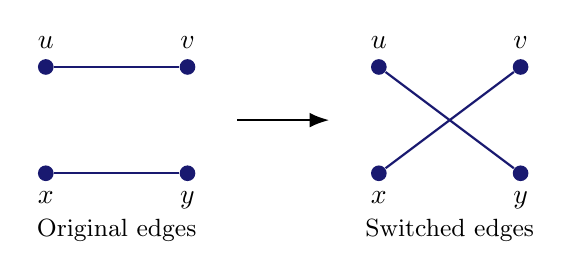
\begin{tikzpicture}[scale=.9,
  vertex/.style={circle,fill=MidnightBlue,inner sep=2pt},
  edge/.style={thick,draw=MidnightBlue}]
\begin{scope}
\node[vertex,label=above:$u$] (u) at (0,1.5) {};
\node[vertex,label=above:$v$] (v) at (2,1.5) {};
\node[vertex,label=below:$x$] (x) at (0,0) {};
\node[vertex,label=below:$y$] (y) at (2,0) {};
\draw[edge] (u)--(v);
\draw[edge] (x)--(y);
\node at (1,-.8) {\small Original edges};
\end{scope}
\draw[-{Latex[length=2.5mm]},thick] (2.7,.75)--(4,.75);
\begin{scope}[xshift=4.7cm]
\node[vertex,label=above:$u$] (u2) at (0,1.5) {};
\node[vertex,label=above:$v$] (v2) at (2,1.5) {};
\node[vertex,label=below:$x$] (x2) at (0,0) {};
\node[vertex,label=below:$y$] (y2) at (2,0) {};
\draw[edge] (u2)--(y2);
\draw[edge] (x2)--(v2);
\node at (1,-.8) {\small Switched edges};
\end{scope}
\end{tikzpicture}
\caption{A degree-preserving switch deletes $uv$ and $xy$ and inserts
$uy$ and $xv$. The four endpoints are distinct, and the inserted
edges must be absent. The crossing in the right panel is not a vertex.
With $U=[e_u-e_x,e_v-e_y]$ and $F$ the two-coordinate swap matrix,
the adjacency change is $-UFU^T$.}
\label{fig:switch}
\end{figure}


For the fixed cutoffs, put
$E_0^\sigma=\operatorname{span}\{v_i:x_i^\sigma<w_B^\sigma\}$, and let
$U_E$ denote the coordinates of $U$ in this subspace.  Define
\begin{equation}
 S_B=C_\sigma^{-1}+U^TR_B^\sigma U.
 \label{eq:original-64}
\end{equation}
The two original edges in a draw each contribute one endpoint block to
$U^TR_B^\sigma U$.  Replacing these by their tree blocks and setting the
cross-edge entries to zero gives the ideal $2$-by-$2$ block
\[
 \sigma F+2P_{\mathrm{tree}}^\sigma
 =\frac1{d-2}
   \begin{pmatrix}s&\sigma d\\ \sigma d&s\end{pmatrix}.
\]
It has determinant $-1$, one eigenvalue of each sign, and inverse
\begin{equation}
 K_\sigma=
 \frac{d}{d-2}\begin{pmatrix}-s/d&\sigma\\ \sigma&-s/d\end{pmatrix}.
 \label{eq:original-65}
\end{equation}
If $S_B$ is sufficiently close in norm to the block diagonal matrix of these
ideal blocks, it has the same inertia as $C_\sigma^{-1}$.
To see why this suffices even when some old near slacks are negative, let
$D_B=\operatorname{diag}_{(E_0^\sigma)^\perp}(x_i^\sigma)>0$ be the
old bulk precision within $\mathbf1^\perp$, and let $U_B$ be the bulk
coordinates of $U$.  The two Schur complements of
\[
 \begin{pmatrix}D_B&U_B\\ U_B^T&-C_\sigma^{-1}\end{pmatrix}
\]
give
\[
 \operatorname{In}(D_B)+\operatorname{In}(-S_B)
 =\operatorname{In}(-C_\sigma^{-1})
   +\operatorname{In}(D_B+U_BC_\sigma U_B^T),
\]
where $\operatorname{In}$ records positive, negative and zero eigenvalue
counts.  The equal middle inertias cancel, proving that the updated bulk
precision $D_B+U_BC_\sigma U_B^T$ is positive definite.
Eliminating this bulk leaves the exact near Schur complement
\begin{equation}
 \operatorname{diag}_{E_0^\sigma}(x_i^\sigma)
       +U_ES_B^{-1}U_E^T.
 \label{eq:original-66}
\end{equation}
This is the Woodbury identity on the positive old bulk
\cite{HS1981}; no positivity of the old near block is required.

\par\smallskip\noindent\textit{Step 2: give the near spectrum a positive mean shift.}\quad
The inverse $K_\sigma$ in \eqref{eq:original-65} determines the ideal
contribution of one switch after the bulk has been eliminated.  Let
$U_{E,g,j}$ denote the near coordinates of the two columns of $U_{g,j}$,
and put
\[
 H^\sigma=U_{E,g,j}K_\sigma U_{E,g,j}^T.
\]
Thus replacing $S_B^{-1}$ in \eqref{eq:original-66} by the block diagonal
matrix with blocks $K_\sigma$ replaces the near correction by
$\sum_{r=1}^M H_r^\sigma$.  Since $K_\sigma$ is indefinite, we must control
this sum through the choice of the edge-pair distribution.

First let $\nu_0$ be the law of two independent uniformly chosen oriented
edges.  For $g=(u,v)$ and nonconstant indices $i$, write
\[
 z_i(g)=(v_i(u),v_i(v))^T,\qquad
 M_i=\begin{pmatrix}1&\lambda_i/d\\ \lambda_i/d&1\end{pmatrix}.
\]
Regularity and orthogonality give
\[
 \mathbb E_{\nu_0}z_i(g)=0,\qquad
 \mathbb E_{\nu_0}[z_i(g)z_k(g)^T]=\frac{\delta_{ik}}n M_i.
\]
For indices in $E_0^\sigma$, the entry of the single-switch correction is
\[
 H_{ik}^\sigma=(z_i(g)-z_i(j))^TK_\sigma(z_k(g)-z_k(j)).
\]
Its uniform mean is
\[
 \mathbb E_{\nu_0}H_{ik}^\sigma
 =\frac{2\delta_{ik}}n\operatorname{Tr}(K_\sigma M_i)
 =-\frac{4\delta_{ik}x_i^\sigma}{(d-2)n}.
\]
Consequently the uniform mean correction only multiplies each old slack by
$1-4M/((d-2)n)>0$.  It cannot turn a negative slack into a positive one.
We therefore bias the correlations between the two edges on the modes
closest to either threshold.

Choose cutoffs $t_T^\tau\in[2e,3e]$ avoiding the signed slacks
$\{x_i^\tau:2\le i\le n\}$, and set
\[
 T_\tau=\{i:x_i^\tau<t_T^\tau\},\qquad
 J_T\asymp n^{3a/2+a/10}.
\]
Define the tilted law $\nu$ by multiplying the $\nu_0$ probabilities by
\begin{equation}
 1+\frac1{B_*}\left[-\frac{2n}{J_T}
       \sum_{\tau=\pm1}\sum_{i\in T_\tau}
       z_i(g)^TK_\tau z_i(j)\right],
 \label{eq:original-67}
\end{equation}
where $B_*>0$ is a sufficiently large fixed constant.
This is a positive probability density.  Indeed,
\eqref{eq:original-61} and Cauchy--Schwarz bound the absolute value of the
bracket by
\[
 C\frac{n e^{3/2}}{J_T}=O(n^{-a/10})=o(1).
\]
Every nonconstant eigenvector has mean zero on either endpoint of a uniform
oriented edge.  The bracket therefore has mean zero under $\nu_0$ even when
either edge is fixed.  The density is normalized and both edge marginals
under $\nu$ remain uniform.

Expansion under this tilted law gives
\begin{equation}
 \mathbb E_\nu H_{ik}^\sigma
 =\delta_{ik}\left[
 -\frac{4x_i^\sigma}{(d-2)n}
 +\frac4{B_*J_Tn}
   \sum_{\tau:\,i\in T_\tau}
      \operatorname{Tr}(K_\sigma M_iK_\tau M_i)
 \right].
 \label{eq:original-68}
\end{equation}
The first term is the uniform mean computed above.  In the tilt correction
only the two cross-edge terms in the expansion of $H_{ik}^\sigma$ survive.
Each forces the two near indices to agree with the tilting index, and each
contributes the same trace divided by $n^2$.  Their negative signs cancel
the negative sign in \eqref{eq:original-67}, giving the displayed factor
$4/(B_*J_Tn)$.

For a $\sigma$-near mode, only $T_\sigma$ can occur in the sum, since the two
signed slacks add to $2s$ and $2W_b+3e=o(1)$.
On these modes $M_i$ is uniformly positive definite, because $s<d$, and
\[
 \operatorname{Tr}(K_\sigma M_iK_\sigma M_i)
 =\|M_i^{1/2}K_\sigma M_i^{1/2}\|_{\mathrm F}^2\ge c_d.
\]
The positive bias satisfies
$M/(J_Tn)\asymp n^{-2/3+8.4a}\gg e$.
It overwhelms the possible slack $-e/20$ on $T_\sigma$.
Outside $T_\sigma$, the slack is at least $2e$, and multiplication by
$1-4M/((d-2)n)=1-o(1)$ preserves a fixed fraction of it.  Thus the same
law improves both signed forms:
\begin{equation}
 \operatorname{diag}(x_i^\sigma)+M\mathbb E_\nu H^\sigma\succeq ceI
 \quad\text{on }E_0^\sigma.
 \label{eq:original-69}
\end{equation}

\par\smallskip\noindent\textit{Step 3: restrict the draws to typical edges.}\quad
For the bulk cutoffs fixed in Step 1, keep only oriented edges whose endpoint
blocks have the required accuracy for both signs.
The numerical implementation below includes every edge with the proven
$n^{-.024}$ accuracy and includes only edges with $Cn^{-.02}$ accuracy.
Condition $\nu$ on both sampled edges lying in this set.  The removed
probability is $O(n^{-.1})$.  Approximate the resulting law in total variation
by $n^{-C}$, for a sufficiently large fixed $C$, retaining a bound
$C_d/(dn)^2$ for every point probability.

For any draw, the projector estimate at scale $2W_b$ gives
\[
 \|U_{E,g,j}\|_{\mathrm F}^2\le CW_b^{3/2},\qquad
 \|H^\sigma\|_{\mathrm F}\le CW_b^{3/2}.
\]
Consequently, the restriction and the probability approximation change the
left side of \eqref{eq:original-69} by at most
\[
 CM(n^{-.1}+n^{-C})W_b^{3/2}=o(e).
\]
Denote the approximating law, including the probability rounding in Step~7,
by $\mu$.  Unlike $\nu$, it need not have exactly uniform marginals; the
pointwise density bound is what the remaining estimates use.

\par\smallskip\noindent\textit{Step 4: control fluctuations and collisions.}\quad
Take $M$ draws with law $\mu$, requiring only pairwise independence between
draws.  The bulk inverse error will be sandwiched by $U_E$, so a bound
$\|U_EU_E^T\|=O(M/n)$ makes $o(en/M)$ the bulk error scale needed to
obtain an $o(e)$ error in the near form.  We prove that, with probability
$1-o(1)$, simultaneously for both signs,
\begin{equation}
 \begin{split}
 &\left\|\sum_{r=1}^M H_r^\sigma-M\mathbb E_\mu H^\sigma\right\|=o(e),\\
 &\|U_EU_E^T\|\le CM/n,\\
 &\left\|S_B-\operatorname{blockdiag}
          (\sigma F+2P_{\mathrm{tree}}^\sigma)\right\|=o(en/M).
 \end{split}
 \label{eq:original-70}
\end{equation}
Here and below a block diagonal notation in this display has $M$ blocks.
We supply all three second-moment estimates.

Pairwise independence makes the cross terms in the squared Frobenius norm of
a centered sum vanish.  Hence
\[
 \mathbb E\left\|\sum_{r=1}^M
 (H_r^\sigma-\mathbb E_\mu H_r^\sigma)\right\|_{\mathrm F}^2
 \le CM W_b^3.
\]
For the sum $U_EU_E^T$ the same estimate applies to its centered version.
Uniform-density domination gives its mean the positive-order bound $CMI/n$:
for any unit vector in the near subspace, average the squares of its four
endpoint values and use that an endpoint of a uniform oriented edge is uniform
on vertices.  Since
\[
 \sqrt M\,W_b^{3/2}=n^{-5/6+155a+o(1)}
       \ll e,\ M/n,
\]
Markov's inequality proves the first two assertions.

To prove the third, first retain the two endpoint blocks belonging to each
separate sampled edge.  They have error $O(n^{-.02})$ by construction; after
forming the difference columns this is still a block-diagonal operator error
$O(n^{-.02})$.
All the other entries concern endpoints in different edge slots.  This
includes the two edge slots within a draw.  Such a pair of edge slots has joint
density bounded by a constant relative to two uniform oriented edges: within
one draw this is the pointwise bound for $\mu$, and between draws it follows
from pairwise independence and the bounded marginal densities.
For any prescribed endpoint in each slot, \eqref{eq:original-63} therefore
gives
\[
 \mathbb E\left| (R_B^\sigma)_{pq}\right|^2
 \le \frac{C}{n^2}\sum_{p,q}|(R_B^\sigma)_{pq}|^2
 \le \frac{C}{n\sqrt{W_b}}.
\]
There are $O(M^2)$ such entries.  Passing from the endpoint columns to their
differences has operator norm $\sqrt2$, so the total squared Frobenius budget
is at most $CM^2/(n\sqrt{W_b})$ up to a fixed factor.  Its square root obeys
\[
 \frac{M}{\sqrt n\,W_b^{1/4}}
   =n^{b_*-t_*/4+o(1)}=n^{-15a+o(1)}
   \ll en/M=n^{-9a+o(1)}.
\]
This is exactly the strict inequality $t_*>8b_*-4a$.
Also $n^{-.02}=o(en/M)$.  Markov's inequality now proves the third assertion
of \eqref{eq:original-70}.  All the displayed separations have a fixed power
margin, so the $o(1)$ probability bounds can be imposed simultaneously.

The same density estimates show that endpoint coincidences within or between
draws, or a proposed new edge already present in $G$, have total probability
$O_d(M^2/n)=n^{-1/3+20a+o(1)}=o(1)$.
Indeed each particular coincidence or adjacency has probability $O_d(1/n)$;
there are $O(M^2)$ pairs of slots.  Original edges have distinct endpoints by
simplicity.  On the complementary event all four endpoints of every switch
are distinct and different switches are vertex-disjoint.  Thus the switches
are simultaneously valid, introduce neither loops nor repeated edges, and
preserve every degree.

The following ratios collect the margins used above.  Fixed factors and
integer rounding do not change their powers of $n$.  The first ratio grows;
every error ratio tends to zero for $a=10^{-4}$.
\begin{center}
\small
\begin{tabular}{@{}lll@{}}
\toprule
Contribution&Comparison scale&Ratio, up to fixed factors\\
\midrule
Mean bias $M/(J_Tn)$&$e$&$n^{7.4a}$\\
Conditioning error $Mn^{-.1}W_b^{3/2}$&$e$&$n^{-.1+159a}$\\
Near fluctuation $\sqrt M\,W_b^{3/2}$&$e$&$n^{-1/6+154a}$\\
Bulk fluctuation $M/(\sqrt n\,W_b^{1/4})$&$en/M$&$n^{-6a}$\\
Typical-block error $n^{-.02}$&$en/M$&$n^{-.02+9a}$\\
Collision probability $M^2/n$&$1$&$n^{-1/3+20a}$\\
\bottomrule
\end{tabular}
\end{center}
Since $e=o(M/n)$, the near-fluctuation estimate also supplies the
second line of \eqref{eq:original-70}.  No common exceptional edge set over
different cutoff pairs is used: the cutoffs were fixed before the law
was conditioned.

\par\smallskip\noindent\textit{Step 5: conclude strict positivity at both edges.}\quad
For a collection satisfying all these conclusions, the inverse perturbation
identity and the bounded inverse in \eqref{eq:original-65} give
\[
 \left\|S_B^{-1}-\operatorname{blockdiag}(K_\sigma)\right\|
 =o(en/M).
\]
Write $\mathcal K_\sigma=\operatorname{blockdiag}(K_\sigma,\ldots,K_\sigma)$.
The near Schur complement is exactly
\[
 \operatorname{diag}(x_i^\sigma)+\sum_{r=1}^M H_r^\sigma
       +U_E(S_B^{-1}-\mathcal K_\sigma)U_E^T.
\]
The last term has norm $o(e)$ by the second line of
\eqref{eq:original-70}.  The centered fluctuation and the change from
$\nu$ to $\mu$ each cost another $o(e)$.  The positive mean bound
\eqref{eq:original-69} therefore makes this Schur complement positive
definite.
The updated bulk was already positive definite.  Thus the full signed
precision is positive definite on $\mathbf 1^\perp$, for both signs.
This proves the asserted strict spectral bounds for at least one collection.

\par\smallskip\noindent\textit{Step 6: compute rational approximations to the law.}\quad
It remains to find such a collection deterministically.  All accuracies in
this paragraph can be $n^{-C}$ for any sufficiently large fixed $C$.
Use the rational matrix
\[
 A_\perp=A_G-d\mathbf 1\mathbf 1^T/n,
\]
which agrees with $A_G$ on $\mathbf 1^\perp$ and has eigenvalue zero on the
constant direction.  For each sign, choose rational cutoffs for the eigenvalues
of $\sigma A_\perp$, with the corresponding slack thresholds in the interiors
of $[W_b,2W_b]$ and $[2e,3e]$, respectively.  These cutoffs can have a gap at
least an inverse polynomial from the spectrum.  To see this, approximate $s$
to much greater precision, place more than $2n$ rational candidates at spacing
comparable to the interval width divided by $n$, and put disjoint small
neighborhoods around them.  At most $n$ neighborhoods can contain eigenvalues.
Exact rational inertia tests at the endpoints, together with a zero-eigenvalue
test at an endpoint, identify an empty neighborhood.  Choosing the candidates
in a fixed interior subinterval ensures that the error in approximating $s$
does not change the required slack interval.

The projectors onto $T_\tau$ and the operators $R_B^\sigma$ can now be
approximated in operator norm without resolving any internal eigenvalue
spacings.  On a fixed rational interval containing $[-d,d]$, define a continuous
cutoff function equal to its required zero or one value outside the separating
gap, with linear interpolation inside the gap.  For the bulk reciprocal use a
very accurate rational $\widetilde s$: set the function equal to
$1/(\widetilde s-t)$ on the bulk side and zero on the excluded side, and
interpolate through the empty gap.  These functions have polynomially bounded
Lipschitz constants and rational values of polynomial bit length at rational
arguments.  The reciprocal approximation has an additional error at most
$C|\widetilde s-s|/W_b^2$, which is made negligible by the chosen precision.

After affine scaling to $[0,1]$, a function with Lipschitz constant $L_f$ has
Bernstein polynomial \cite{Bernstein1912} of degree $D$ with uniform error at most
$L_f/(2\sqrt D)$.  This follows by writing the Bernstein polynomial as
$\mathbb E f(X/D)$ for $X\sim\operatorname{Bin}(D,t)$ and applying
Cauchy--Schwarz to $\mathbb E|X/D-t|$.
Take a polynomially large degree $D$ to obtain the desired inverse-polynomial
accuracy, and evaluate these rational polynomials at $\sigma A_\perp$.
The spectral theorem transfers the scalar error to operator norm.
Sandwich the resulting operators by $I-\mathbf 1\mathbf 1^T/n$ to remove the
artificial constant eigenvalue.  Rational matrix-polynomial evaluation has
polynomial bit complexity: the degree is polynomial, its coefficients have
polynomial bit length, and direct products and sums increase bit lengths by
at most polynomial factors.

Use the approximate bulk blocks and approximate
$P_{\mathrm{tree}}^\sigma$ to accept all edges with the proved
$n^{-.024}$ accuracy and only edges with $Cn^{-.02}$ accuracy.  For example,
use a rational entrywise threshold between these two scales; the approximation
error is much smaller than either threshold.  The sum in the tilt is
basis-invariant: for endpoint indices $g_r,j_t$ it equals
\[
 \sum_{r,t=1}^2(K_\tau)_{rt}
       (\operatorname{Proj}_{T_\tau})_{g_r,j_t}.
\]
Thus the approximate projectors and rational approximations to $K_\tau$
give rational positive weights for every accepted edge pair.  Normalize these
weights.  Errors can be made small enough, including the factor $n/J_T$, that
the law is within $n^{-C}$ in total variation of the conditional tilted law.
Its point probabilities remain bounded by $C_d/(dn)^2$.

\par\smallskip\noindent\textit{Step 7: enumerate a polynomial sample space.}\quad
Choose a prime $P$ between $n^{C'}$ and $2n^{C'}$, up to immaterial rounding,
where $C'$ is a sufficiently large fixed constant and $P>M$.
Bertrand's theorem and deterministic trial search provide such a prime in
time polynomial in $n$.
There are $O_d(n^2)$ accepted ordered edge-pair outcomes.  Floor their
probabilities times $P$, then distribute the remaining counts among the
largest fractional remainders.  The counts are nonnegative, sum to $P$,
and differ by at most one from their unrounded values; outcomes outside
the accepted support retain count zero.  Assign that many residues
of $\mathbb F_P$ to each outcome.  The total variation error is
$O_d(n^2/P)$ and the maximum probability increases by at most $1/P$; both are
within the stipulated bounds for large enough $C'$.
Choose the preceding approximation precision and $C'$ so that their combined
total-variation error is at most $n^{-C}$.  The resulting rounded law is a
choice of $\mu$ with all the properties used in Steps 3--5.

Use the standard affine construction of pairwise-independent variables
(see \cite[Section~2.2]{PR2008}).  Enumerate all $P^2$ seeds
$(\gamma,\beta)\in\mathbb F_P^2$ and use the residues
\[
 \gamma r+\beta\qquad(1\le r\le M)
\]
to select the draws.  Under a uniform seed, any two residues are independent
and uniform: for $r\ne t$, the map
$(\gamma,\beta)\mapsto(\gamma r+\beta,\gamma t+\beta)$ is bijective since
$r-t\ne0$ in $\mathbb F_P$.  Mapping residues to outcomes preserves pairwise
independence.  The estimates above therefore prove that a positive fraction,
indeed a fraction $1-o(1)$, of these seeds satisfy all the required events.

For each seed, discard collections with intersecting endpoint sets or an
invalid switch, build the candidate graph, and test its spectrum exactly.
A rational contrast basis tests the positivity
of
\[
 4qI-A_{G'}^2\quad\text{on }\mathbf 1^\perp
\]
by exact rational congruence and inertia.  Positive definiteness gives the
strict conclusion of the theorem.  Symmetric elimination uses a nonzero
diagonal pivot if available, otherwise an invertible off-diagonal
$2$-by-$2$ pivot, with a remaining zero block contributing zero eigenvalues.
Fraction-free arithmetic or determinant bounds keep all intermediate bit
lengths polynomial: Schur-complement entries are ratios of minors of the
original pivoted rational matrix.  The same procedure implements the cutoff
tests above.  A passing seed exists by the preceding argument, and the number
of seeds and all work per seed are polynomial in $n$.

Finally, $d>2\sqrt{d-1}$.  A disconnected regular graph has an additional
$d$-eigenvector orthogonal to $\mathbf 1$, and a bipartite regular graph has a
$-d$-eigenvector.  The verified strict bound excludes both possibilities.
\end{proof}

\begin{remark}[Inputs supplied by the pairing construction]
The theorem uses only the three stated properties of $G$.
The completed pairing supplies $x_i^\sigma>-e/20$ and the final entry
comparison.  Its frozen-reference conclusions verify
Lemma~\ref{lem:repair-projector}; its separation-stop path estimates verify
the typical-edge assertion in Lemma~\ref{lem:repair-bulk}.  The repair therefore
applies to precisely the graph constructed in the preceding sections, with
no change of vertex set.
\end{remark}

\section{The algorithm and its bit complexity}\label{sec:algorithm}

The preceding sections prove existence of a successful choice at every
stage. During pairing, the algorithm chooses a minimizer of the discounted
accounts; during repair, it enumerates a polynomial family of simultaneous
switches and accepts the first graph passing an exact spectral test.
We now verify that these operations fit the stated bit model, and then
assemble the theorem. All computations use rational
numbers, except for real quantities used solely to analyze their bounds.


\begin{proposition}\label{prop:bit-complexity}
For each fixed $d$ and the fixed choices in Section~\ref{subsec:hierarchy}, every
stage of the preceding construction is implementable with polynomially
many bit operations in $n$.
\end{proposition}

\begin{proof}
\textit{Rational parameters.}
Choose dyadic rational representatives for all power scales, within the
fixed factors allowed above.  Comparisons for a fixed rational exponent
can be made by integer powers, so these representatives require
$O_d(\log n)$ bits and are computable in polynomial time.  Integer power
comparisons similarly determine the logarithmic radii.  Approximate the
primary $h$ values to sufficiently high inverse-polynomial precision,
strictly below $1/\sqrt q$; choose the small auxiliary spacings rationally
and exactly equally spaced where required.  The strict exponent margins
preserve every estimate.  The piecewise-polynomial cutoff for the smooth
reference can have rational breakpoints and coefficients and fixed
finite smoothness, for example by rescaling the integral of
$t^j(1-t)^j$ at its transition intervals.  Its Fourier transform is used
only in the proof of an estimate, never by the algorithm.

\textit{Candidate computations.}
There are at most $O_d(n^2)$ choices at a pairing step and $O_d(n)$ steps.
Distances, stub eligibility, and exceptional-event flags are finite graph
computations.  The precision matrices have rational entries of
polynomial bit length.  Their inverses on $\mathbf1^\perp$ can be
computed in a rational contrast basis or after adding the constant
projection.  The coefficients of the path series are computed from the
displayed matrix recurrence, of length $O_d(\log n)$.  The frozen
reference is evaluated from its explicit Woodbury formula at the current
matching, rather than through an uncontrolled sequence of rational
expansions.

The structural completion estimators are computed with the colorful
dynamic program described in the structural section.  Its shapes have
$O_d(\log n)$ vertices and bounded treewidth once the fixed excess cutoff
has been chosen.  The factor $2^{O(k)}$ for the color subset and the
$\exp(k)k^{O(\log k)}\log n$ hash-family size are polynomial in $n$ when
$k=O_d(\log n)$.  Pending-edge probabilities are rational products with
$O_d(\log n)$ factors.  These observations give polynomial time and bit
length for every such estimator.

All moments have fixed integer order.  Traces, squares, even powers,
positive parts of rational numbers, comparator values, and uniform
conditional expectations are therefore rational and computable in
polynomial time.  There are polynomially many accounts, including the
fixed contrast labels and their pairs.

\textit{Discounts.}
At a step the expectation ratio for an account is computed from its
undiscounted local statistic, its fixed phase baseline, and its
comparator and event flags.  It is not computed recursively from the
discounted total.  A sum over the polynomially many candidates has
polynomial bit length.  A discount is a product of polynomially many
such ratios; consequently it too has polynomial bit length.  Dynamic
comparators are explicit rational functions or products of polynomially
many polynomial-bit factors.  Sums and comparisons of the discounted
accounts can thus be carried out exactly.

For completeness, the polynomial bit bounds for static matrix inverses
follow from the determinant formula: after a common denominator is
cleared, minors of a polynomial-bit matrix of dimension $O_d(n)$ have
polynomial bit length by the determinant bound.  Exact rational symmetric
inertia can be computed by a nonzero diagonal pivot, or, if all diagonals
vanish and a nonzero off-diagonal remains, by an invertible $2$-by-$2$
pivot.  The remaining zero block contributes zero eigenvalues.
Fraction-free elimination \cite[Section~I]{Bareiss1968} or the minor formulas
give the same bit bound
for intermediate quantities.

\textit{Repair and verification.}
The repair section constructs inverse-polynomially separated cutoffs,
rational polynomial approximations to the required spectral functions,
and a polynomial-size prime-field sample space.  Enumerating that sample
space and performing the graph updates therefore takes polynomial time.
The precision exponent is fixed after the analytic margins have been
chosen.  In particular, after affine rescaling to $[0,1]$, if a spectral
cutoff function has a known Lipschitz bound $L_f\le n^c$ and the target
error is $n^{-C}$, its
Bernstein approximation may be taken of degree
$D=\lceil n^{2(c+C)}\rceil$, polynomial in $n$ for fixed $c,C$.
Its rational sample values and polynomial coefficients have polynomial
bit length.  Increasing the fixed precision and prime-denominator
exponents pays for both the tilt factor $n/J_T$ and the total
probability-rounding error.

For each simple regular candidate, take the explicit rational contrast basis
\[
 B=[e_1-e_n,\ldots,e_{n-1}-e_n].
\]
Its columns are linearly independent and span $\mathbf1^\perp$.
The condition
\[
 B^T(4qI-A_G^2)B
 =4qB^TB-(A_GB)^T(A_GB)\succ0
\]
is equivalent to the strict nontrivial spectral bound and is decidable
by exact rational inertia.  Indeed, this congruence tests the quadratic
form on all of $\mathbf1^\perp$; an orthonormal basis is unnecessary.
Regularity makes that subspace invariant under $A_G$, so the form is
positive exactly when every eigenvalue there has square less than $4q$.
The repair theorem guarantees that the search
finds a passing candidate with a strict spectral inequality.

All constants, polynomial degrees, moment orders, and approximation
exponents depend only on $d$.  A sufficiently large finite exponent
$k_d$ bounds their combined bit cost.  This bound holds once the finitely many large-$n$ requirements are met.
\end{proof}

\begin{proof}[Proof of Theorem~\ref{thm:main}]
Start with $d$ distinguishable stubs at each of $n$ vertices.  Apply
Proposition~\ref{prop:early-phase}, rejecting stub
pairs whose vertices have distance at most the girth exclusion radius.
The rejected-pair graph has maximum degree $O_d(q^{g_0})=o(l_0)$, so the
candidate set is nonempty throughout this phase.  Apply
Proposition~\ref{prop:cleanup} to reach $l_0$ unresolved stubs.  The structural estimates guarantee that
these stubs lie at distinct vertices and are mutually separated, with
no nonempty short nonbacktracking return at any remaining vertex.

The reference construction and Proposition~\ref{prop:boundary-completion} then complete the
configuration to a simple $d$-regular graph.  For every primary parameter
and both signs, its precision is positive; at the closest parameter this
gives
\[
 \|A_G|_{\mathbf1^\perp}\|<s+e/20.
\]
The final entry comparison and the diagonal derivative bound for the same
frozen reference give the local spectral mass estimate by
Lemma~\ref{lem:repair-projector}.  The retained path estimates at the
separation stop, together with that entry comparison, give the typical
bulk edge blocks by Lemma~\ref{lem:repair-bulk}.  These are precisely the
remaining hypotheses of Theorem~\ref{thm:exact-repair}.  Apply that theorem.  This produces a simple
$d$-regular graph on the same $n$ vertices with every nonconstant
eigenvalue strictly in $(-s,s)$.

The exact-repair theorem also proves connectedness and nonbipartiteness.
Proposition~\ref{prop:bit-complexity} supplies a finite exponent $k_d$
for the bit cost. Choose $n_0(d)$ to satisfy the finitely many
large-$n$ requirements in the construction. This proves all parts of
Theorem~\ref{thm:main}.
\end{proof}

\clearpage
\begingroup
\small
\begin{thebibliography}{HMY24}
\raggedright

\bibitem[Alo86]{Alon1986}
Noga Alon.
\newblock Eigenvalues and expanders.
\newblock \emph{Combinatorica}, 6(2):83--96, 1986.
\newblock \href{https://doi.org/10.1007/BF02579166}{doi:10.1007/BF02579166}.

\bibitem[Alo21]{Alon2021}
Noga Alon.
\newblock Explicit expanders of every degree and size.
\newblock \emph{Combinatorica}, 41(4):447--463, 2021.
\newblock \href{https://doi.org/10.1007/s00493-020-4429-x}{doi:10.1007/s00493-020-4429-x}.

\bibitem[AYZ95]{AYZ1995}
Noga Alon, Raphael Yuster, and Uri Zwick.
\newblock Color-coding.
\newblock \emph{Journal of the ACM}, 42(4):844--856, 1995.
\newblock \href{https://doi.org/10.1145/210332.210337}{doi:10.1145/210332.210337}.

\bibitem[Bar68]{Bareiss1968}
Erwin~H. Bareiss.
\newblock Sylvester's identity and multistep integer-preserving Gaussian elimination.
\newblock \emph{Mathematics of Computation}, 22(103):565--578, 1968.
\newblock \href{https://doi.org/10.1090/S0025-5718-1968-0226829-0}{doi:10.1090/S0025-5718-1968-0226829-0}.

\bibitem[BHY19]{BHY2019}
Roland Bauerschmidt, Jiaoyang Huang, and Horng-Tzer Yau.
\newblock Local Kesten--McKay law for random regular graphs.
\newblock \emph{Communications in Mathematical Physics}, 369(2):523--636, 2019.
\newblock \href{https://doi.org/10.1007/s00220-019-03345-3}{doi:10.1007/s00220-019-03345-3}.

\bibitem[Ber12]{Bernstein1912}
S. Bernstein.
\newblock D\'emonstration du th\'eor\`eme de Weierstrass fond\'ee sur le calcul des probabilit\'es.
\newblock \emph{Communications de la Soci\'et\'e math\'ematique de Kharkow},
  second series, 13(1):1--2, 1912.
\newblock \href{https://www.mathnet.ru/eng/khmo107}{Math-Net.Ru: khmo107}.

\bibitem[BL06]{BL2006}
Yonatan Bilu and Nathan Linial.
\newblock Lifts, discrepancy and nearly optimal spectral gap.
\newblock \emph{Combinatorica}, 26(5):495--519, 2006.
\newblock \href{https://doi.org/10.1007/s00493-006-0029-7}{doi:10.1007/s00493-006-0029-7}.

\bibitem[Bor20]{Bordenave2020}
Charles Bordenave.
\newblock A new proof of Friedman's second eigenvalue theorem and its
  extension to random lifts.
\newblock \emph{Annales scientifiques de l'\'Ecole normale sup\'erieure},
  (4) 53(6):1393--1439, 2020.
\newblock \href{https://doi.org/10.24033/asens.2450}{doi:10.24033/asens.2450}.

\bibitem[CM26]{CM2026}
Gil Cohen and Gal Maor.
\newblock Quantitative results on super-Ramanujan graphs.
\newblock Electronic Colloquium on Computational Complexity, Report TR26-163,
  September 2026.
\newblock \url{https://eccc.weizmann.ac.il/report/2026/163/}.

\bibitem[Coh16]{Cohen2016}
Michael~B. Cohen.
\newblock Ramanujan graphs in polynomial time.
\newblock In \emph{Proceedings of the 57th Annual IEEE Symposium on
  Foundations of Computer Science}, pages 276--281, 2016.
\newblock \href{https://doi.org/10.1109/FOCS.2016.37}{doi:10.1109/FOCS.2016.37}.

\bibitem[FZ99]{FZ1999}
Dominique Foata and Doron Zeilberger.
\newblock A combinatorial proof of Bass's evaluations of the
  Ihara--Selberg zeta function for graphs.
\newblock \emph{Transactions of the American Mathematical Society},
  351(6):2257--2274, 1999.
\newblock \href{https://doi.org/10.1090/S0002-9947-99-02234-5}{doi:10.1090/S0002-9947-99-02234-5}.
\newblock Section locators refer to
\href{https://arxiv.org/abs/math/9806037v1}{arXiv:math/9806037v1}.

\bibitem[Fri08]{Friedman2008}
Joel Friedman.
\newblock \emph{A Proof of Alon's Second Eigenvalue Conjecture and Related Problems}.
\newblock Memoirs of the American Mathematical Society, 195(910), 2008.
\newblock \href{https://doi.org/10.1090/memo/0910}{doi:10.1090/memo/0910}.

\bibitem[HPS18]{HPS2018}
Chris Hall, Doron Puder, and William~F. Sawin.
\newblock Ramanujan coverings of graphs.
\newblock \emph{Advances in Mathematics}, 323:367--410, 2018.
\newblock \href{https://doi.org/10.1016/j.aim.2017.10.042}{doi:10.1016/j.aim.2017.10.042}.
\newblock Theorem locators refer to
\href{https://arxiv.org/abs/1506.02335v4}{arXiv:1506.02335v4}.

\bibitem[HS81]{HS1981}
H.~V. Henderson and S.~R. Searle.
\newblock On deriving the inverse of a sum of matrices.
\newblock \emph{SIAM Review}, 23(1):53--60, 1981.
\newblock \href{https://doi.org/10.1137/1023004}{doi:10.1137/1023004}.

\bibitem[HMY24]{HMY2024}
Jiaoyang Huang, Theo McKenzie, and Horng-Tzer Yau.
\newblock Ramanujan property and edge universality of random regular graphs.
\newblock Preprint, 2024; revised February 2025.
\newblock \href{https://arxiv.org/abs/2412.20263v2}{arXiv:2412.20263v2}.

\bibitem[HY24]{HY2024}
Jiaoyang Huang and Horng-Tzer Yau.
\newblock Spectrum of random $d$-regular graphs up to the edge.
\newblock \emph{Communications on Pure and Applied Mathematics},
  77(3):1635--1723, 2024.
\newblock \href{https://doi.org/10.1002/cpa.22176}{doi:10.1002/cpa.22176}.
\newblock Section locators refer to
\href{https://arxiv.org/abs/2102.00963v3}{arXiv:2102.00963v3}.

\bibitem[JSS26]{JSS2026}
Ali Jadbabaie, Amin Saberi, and Suvrit Sra.
\newblock Kadison--Singer partitions and Bilu--Linial graph signings
  in polynomial time.
\newblock Preprint, September 2026.
\newblock \href{https://arxiv.org/abs/2609.23855v1}{arXiv:2609.23855v1}.

\bibitem[LPS88]{LPS1988}
Alexander Lubotzky, Ralph Phillips, and Peter Sarnak.
\newblock Ramanujan graphs.
\newblock \emph{Combinatorica}, 8(3):261--277, 1988.
\newblock \href{https://doi.org/10.1007/BF02126799}{doi:10.1007/BF02126799}.

\bibitem[MSS15]{MSS2015}
Adam~W. Marcus, Daniel~A. Spielman, and Nikhil Srivastava.
\newblock Interlacing families I: Bipartite Ramanujan graphs of all degrees.
\newblock \emph{Annals of Mathematics}, 182(1):307--325, 2015.
\newblock \href{https://doi.org/10.4007/annals.2015.182.1.7}{doi:10.4007/annals.2015.182.1.7}.

\bibitem[MSS18]{MSS2018}
Adam~W. Marcus, Daniel~A. Spielman, and Nikhil Srivastava.
\newblock Interlacing families IV: Bipartite Ramanujan graphs of all sizes.
\newblock \emph{SIAM Journal on Computing}, 47(6):2488--2509, 2018.
\newblock \href{https://doi.org/10.1137/16M106176X}{doi:10.1137/16M106176X}.

\bibitem[Mar88]{Margulis1988}
G.~A. Margulis.
\newblock Explicit group-theoretical constructions of combinatorial schemes
  and their application to the design of expanders and concentrators.
\newblock \emph{Problems of Information Transmission}, 24(1):39--46, 1988.
\newblock Russian original: \emph{Problemy Peredachi Informatsii},
  24(1):51--60, 1988.
\newblock \href{https://www.mathnet.ru/eng/ppi686}{Math-Net.Ru: ppi686}.

\bibitem[MW90]{MW1990}
Brendan~D. McKay and Nicholas~C. Wormald.
\newblock Uniform generation of random regular graphs of moderate degree.
\newblock \emph{Journal of Algorithms}, 11(1):52--67, 1990.
\newblock \href{https://doi.org/10.1016/0196-6774(90)90029-E}{doi:10.1016/0196-6774(90)90029-E}.

\bibitem[MOP22]{MOP2020}
Sidhanth Mohanty, Ryan O'Donnell, and Pedro Paredes.
\newblock Explicit near-Ramanujan graphs of every degree.
\newblock \emph{SIAM Journal on Computing}, 51(3):STOC20-1--STOC20-23, 2022.
\newblock \href{https://doi.org/10.1137/20M1342112}{doi:10.1137/20M1342112}.

\bibitem[Mor94]{Morgenstern1994}
Moshe Morgenstern.
\newblock Existence and explicit constructions of $q+1$ regular Ramanujan
  graphs for every prime power $q$.
\newblock \emph{Journal of Combinatorial Theory, Series B}, 62(1):44--62, 1994.
\newblock \href{https://doi.org/10.1006/jctb.1994.1054}{doi:10.1006/jctb.1994.1054}.

\bibitem[NSS95]{NSS1995}
Moni Naor, Leonard~J. Schulman, and Aravind Srinivasan.
\newblock Splitters and near-optimal derandomization.
\newblock In \emph{Proceedings of the 36th Annual Symposium on Foundations
  of Computer Science}, pages 182--191. IEEE Computer Society Press, 1995.
\newblock \href{https://doi.org/10.1109/SFCS.1995.492475}{doi:10.1109/SFCS.1995.492475}.
\newblock Theorem and section locators refer to the
\href{https://www.wisdom.weizmann.ac.il/~naor/PAPERS/splitters.pdf}{authors' preliminary version}.

\bibitem[Nil91]{Nilli1991}
A.~Nilli.
\newblock On the second eigenvalue of a graph.
\newblock \emph{Discrete Mathematics}, 91(2):207--210, 1991.
\newblock \href{https://doi.org/10.1016/0012-365X(91)90112-F}{doi:10.1016/0012-365X(91)90112-F}.

\bibitem[PR08]{PR2008}
Seth Pettie and Vijaya Ramachandran.
\newblock Randomized minimum spanning tree algorithms using exponentially
  fewer random bits.
\newblock \emph{ACM Transactions on Algorithms}, 4(1):Article~5, 27 pages, 2008.
\newblock \href{https://doi.org/10.1145/1328911.1328916}{doi:10.1145/1328911.1328916}.

\bibitem[Rag88]{Raghavan1988}
Prabhakar Raghavan.
\newblock Probabilistic construction of deterministic algorithms:
  Approximating packing integer programs.
\newblock \emph{Journal of Computer and System Sciences}, 37(2):130--143, 1988.
\newblock \href{https://doi.org/10.1016/0022-0000(88)90003-7}{doi:10.1016/0022-0000(88)90003-7}.

\bibitem[WX08]{WX2008}
Avi Wigderson and David Xiao.
\newblock Derandomizing the Ahlswede--Winter matrix-valued Chernoff bound
  using pessimistic estimators, and applications.
\newblock \emph{Theory of Computing}, 4:53--76, 2008.
\newblock \href{https://doi.org/10.4086/toc.2008.v004a003}{doi:10.4086/toc.2008.v004a003}.

\end{thebibliography}
\endgroup

\end{document}
